\documentclass{article}\usepackage[]{graphicx}\usepackage[]{color}
%% maxwidth is the original width if it is less than linewidth
%% otherwise use linewidth (to make sure the graphics do not exceed the margin)
\makeatletter
\def\maxwidth{ %
  \ifdim\Gin@nat@width>\linewidth
    \linewidth
  \else
    \Gin@nat@width
  \fi
}
\makeatother

\definecolor{fgcolor}{rgb}{0.345, 0.345, 0.345}
\newcommand{\hlnum}[1]{\textcolor[rgb]{0.686,0.059,0.569}{#1}}%
\newcommand{\hlstr}[1]{\textcolor[rgb]{0.192,0.494,0.8}{#1}}%
\newcommand{\hlcom}[1]{\textcolor[rgb]{0.678,0.584,0.686}{\textit{#1}}}%
\newcommand{\hlopt}[1]{\textcolor[rgb]{0,0,0}{#1}}%
\newcommand{\hlstd}[1]{\textcolor[rgb]{0.345,0.345,0.345}{#1}}%
\newcommand{\hlkwa}[1]{\textcolor[rgb]{0.161,0.373,0.58}{\textbf{#1}}}%
\newcommand{\hlkwb}[1]{\textcolor[rgb]{0.69,0.353,0.396}{#1}}%
\newcommand{\hlkwc}[1]{\textcolor[rgb]{0.333,0.667,0.333}{#1}}%
\newcommand{\hlkwd}[1]{\textcolor[rgb]{0.737,0.353,0.396}{\textbf{#1}}}%

\usepackage{framed}
\makeatletter
\newenvironment{kframe}{%
 \def\at@end@of@kframe{}%
 \ifinner\ifhmode%
  \def\at@end@of@kframe{\end{minipage}}%
  \begin{minipage}{\columnwidth}%
 \fi\fi%
 \def\FrameCommand##1{\hskip\@totalleftmargin \hskip-\fboxsep
 \colorbox{shadecolor}{##1}\hskip-\fboxsep
     % There is no \\@totalrightmargin, so:
     \hskip-\linewidth \hskip-\@totalleftmargin \hskip\columnwidth}%
 \MakeFramed {\advance\hsize-\width
   \@totalleftmargin\z@ \linewidth\hsize
   \@setminipage}}%
 {\par\unskip\endMakeFramed%
 \at@end@of@kframe}
\makeatother

\definecolor{shadecolor}{rgb}{.97, .97, .97}
\definecolor{messagecolor}{rgb}{0, 0, 0}
\definecolor{warningcolor}{rgb}{1, 0, 1}
\definecolor{errorcolor}{rgb}{1, 0, 0}
\newenvironment{knitrout}{}{} % an empty environment to be redefined in TeX

\usepackage{alltt}
\usepackage{geometry}
\usepackage{amsmath}
\usepackage{lscape}
\geometry{verbose,tmargin=2.5cm,bmargin=2.5cm,lmargin=2.5cm,rmargin=2.5cm}
\IfFileExists{upquote.sty}{\usepackage{upquote}}{}
\begin{document}




\begin{knitrout}
\definecolor{shadecolor}{rgb}{0.969, 0.969, 0.969}\color{fgcolor}\begin{kframe}
\begin{alltt}
\hlkwd{library}\hlstd{(flexsurv)}
\hlkwd{library}\hlstd{(boot)}
\hlkwd{library}\hlstd{(randomForestSRC)}
\hlkwd{library}\hlstd{(timeROC)}
\hlkwd{library}\hlstd{(risksetROC)}
\hlkwd{source}\hlstd{(}\hlstr{"stdca.R"}\hlstd{)}
\end{alltt}
\end{kframe}
\end{knitrout}


\section{Preparation}
Construct a *preoperative* function based on the Brennan nomogram.  The preoperative nature will mean that most prognostic components will need to be marginalized out.

\begin{table}[h]
\begin{tabular}{llll}
Variable            & Preoperative? & Available? & Marginals                                                                                     \\
Age                 & Yes           & Yes        & Linear.  90 =\textgreater 0, 30 =\textgreater 8.  Therefore $f(x) = -2/15(x-90) = -2/15x + 12$ \\
Sex                 & Yes           & Yes        & Male risk delta 3                                                                             \\
Portal Vein         & NO            &            & 14.4\% YES, risk delta 10, marginal 1.4                                                       \\
Splenectomy         & NO            &            & 9.9\% YES, risk delta 62, marginal 6.1                                                        \\
Margin of resection & NO            &            & 20.7\% POS, risk delta 4, marginal 0.8                                                        \\
Head.vs.Other       & Yes           & Yes        & Head risk delta 51                                                                            \\
Differentiation     & NO            &            & 14.2\% Well, risk delta 0, marginal 0                                                         \\
                    &               &            & 56.4\% Mod, risk delta 14, marginal 7.9                                                       \\
                    &               &            & 29.5\% Poor, risk delta 35, marginal 10.3.  Overall marginal 18.2                             \\
Posterior.margin    & NO            &            & 86.0\% POS, risk delta 22, marginal 18.9                                                      \\
Numb.pos.nodes      & NO            &            & Mean 2.1, approx marginal 15                                                                  \\
Numb.neg.nodes      & NO            &            & Mean 16.9, approx marginal 9                                                                  \\
Back.pain           & Yes           & NO         & 13.7\% YES, risk delta 15, marginal 2.0                                                       \\
T.stage             & Yes           & Yes        &                                                                                               \\
Weight Loss         & Yes           & NO         & 53.7\% YES, risk delta 3,  marginal 1.6                                                       \\
Max.path.axis       & Yes           & Yes        &                                                                                              
\end{tabular}
\end{table}

So the preoperative MSKCC score would be:
\begin{align}
S &= 1.4 + 6.1 + 0.8 + 18.2 + 18.9 + 15 + 9 + 15*Back.pain + 3*Weight.Loss + -2/15*Age + 12 + 3\left[Sex = M\right] + 51\left[Head.vs.Other = Head\right] + T.stage + Max.path.axis
  &= 81.4 + 15*Back.pain + 3*Weight.Loss + -2/15*Age + 3*\left[Sex = M\right] + 51\left[Head.vs.Other = Head\right] + fT(T.stage) + fS(Max.path.axis)
fT(T.stage) = 36\left[T.stage = T1\right] + 10\left[T.stage = T3\right] + 63\left[T.stage = T4\right]
\end{align}


\begin{knitrout}
\definecolor{shadecolor}{rgb}{0.969, 0.969, 0.969}\color{fgcolor}\begin{kframe}
\begin{alltt}
\hlstd{fit.mskcc} \hlkwb{=} \hlkwd{list}\hlstd{(}
        \hlkwc{inputs} \hlstd{=} \hlkwd{list}\hlstd{(}
        \hlkwc{History.Diagnosis.AgeAt} \hlstd{=} \hlkwd{list}\hlstd{(}
                \hlkwc{margins} \hlstd{=} \hlkwd{data.frame}\hlstd{(}\hlkwc{value} \hlstd{=} \hlnum{65}\hlstd{,} \hlkwc{fraction} \hlstd{=} \hlnum{1}\hlstd{),}
                \hlkwc{scorefunc} \hlstd{=} \hlkwa{function}\hlstd{(}\hlkwc{x}\hlstd{) \{ x} \hlkwb{=} \hlstd{x;} \hlopt{-}\hlnum{2}\hlopt{/}\hlnum{15}\hlopt{*}\hlkwd{pmin}\hlstd{(}\hlkwd{pmax}\hlstd{(x,} \hlnum{0}\hlstd{),} \hlnum{90}\hlstd{)} \hlopt{+} \hlnum{12} \hlstd{\}),}
        \hlkwc{Patient.Sex} \hlstd{=} \hlkwd{list}\hlstd{(}
                \hlkwc{margins} \hlstd{=} \hlkwd{data.frame}\hlstd{(}\hlkwc{value} \hlstd{=} \hlkwd{c}\hlstd{(}\hlstr{"M"}\hlstd{,} \hlstr{"F"}\hlstd{),} \hlkwc{fraction} \hlstd{=} \hlkwd{c}\hlstd{(}\hlnum{0.501}\hlstd{,} \hlnum{1}\hlopt{-}\hlnum{0.501}\hlstd{)),}
                \hlkwc{scorefunc} \hlstd{=} \hlkwa{function}\hlstd{(}\hlkwc{x}\hlstd{) \{} \hlnum{3}\hlopt{*}\hlkwd{I}\hlstd{(x} \hlopt{==} \hlstr{"M"}\hlstd{) \}),}
        \hlkwc{Portal.Vein} \hlstd{=} \hlkwd{list}\hlstd{(}
                \hlkwc{margins} \hlstd{=} \hlkwd{data.frame}\hlstd{(}\hlkwc{value} \hlstd{=} \hlkwd{c}\hlstd{(}\hlnum{TRUE}\hlstd{,} \hlnum{FALSE}\hlstd{),} \hlkwc{fraction} \hlstd{=} \hlkwd{c}\hlstd{(}\hlnum{0.144}\hlstd{,} \hlnum{1}\hlopt{-}\hlnum{0.144}\hlstd{)),}
                \hlkwc{scorefunc} \hlstd{=} \hlkwa{function}\hlstd{(}\hlkwc{x}\hlstd{) \{} \hlnum{10}\hlopt{*}\hlkwd{I}\hlstd{(x} \hlopt{==} \hlnum{TRUE}\hlstd{) \}),}
        \hlkwc{Splenectomy} \hlstd{=} \hlkwd{list}\hlstd{(}
                \hlkwc{margins} \hlstd{=} \hlkwd{data.frame}\hlstd{(}\hlkwc{value} \hlstd{=} \hlkwd{c}\hlstd{(}\hlnum{TRUE}\hlstd{,} \hlnum{FALSE}\hlstd{),} \hlkwc{fraction} \hlstd{=} \hlkwd{c}\hlstd{(}\hlnum{0.099}\hlstd{,} \hlnum{1}\hlopt{-}\hlnum{0.099}\hlstd{)),}
                \hlkwc{scorefunc} \hlstd{=} \hlkwa{function}\hlstd{(}\hlkwc{x}\hlstd{) \{} \hlnum{62}\hlopt{*}\hlkwd{I}\hlstd{(x} \hlopt{==} \hlnum{TRUE}\hlstd{) \}),}
        \hlkwc{Treat.MarginPositive} \hlstd{=} \hlkwd{list}\hlstd{(}
                \hlkwc{margins} \hlstd{=} \hlkwd{data.frame}\hlstd{(}\hlkwc{value} \hlstd{=} \hlkwd{c}\hlstd{(}\hlnum{TRUE}\hlstd{,} \hlnum{FALSE}\hlstd{),} \hlkwc{fraction} \hlstd{=} \hlkwd{c}\hlstd{(}\hlnum{0.207}\hlstd{,} \hlnum{1}\hlopt{-}\hlnum{0.207}\hlstd{)),}
                \hlkwc{scorefunc} \hlstd{=} \hlkwa{function}\hlstd{(}\hlkwc{x}\hlstd{) \{} \hlnum{4}\hlopt{*}\hlkwd{I}\hlstd{(x} \hlopt{==} \hlnum{TRUE}\hlstd{) \}),}
        \hlkwc{Path.LocationBody} \hlstd{=} \hlkwd{list}\hlstd{(}
                \hlkwc{margins} \hlstd{=} \hlkwd{data.frame}\hlstd{(}\hlkwc{value} \hlstd{=} \hlkwd{c}\hlstd{(}\hlnum{FALSE}\hlstd{,} \hlnum{TRUE}\hlstd{),} \hlkwc{fraction} \hlstd{=} \hlkwd{c}\hlstd{(}\hlnum{0.894}\hlstd{,} \hlnum{1}\hlopt{-}\hlnum{0.894}\hlstd{)),}
                \hlkwc{scorefunc} \hlstd{=} \hlkwa{function}\hlstd{(}\hlkwc{x}\hlstd{) \{} \hlnum{51}\hlopt{*}\hlkwd{I}\hlstd{(x} \hlopt{==} \hlnum{TRUE}\hlstd{) \}),}
        \hlkwc{Path.Differentiation} \hlstd{=} \hlkwd{list}\hlstd{(}
                \hlkwc{margins} \hlstd{=} \hlkwd{data.frame}\hlstd{(}\hlkwc{value} \hlstd{=} \hlkwd{c}\hlstd{(}\hlstr{"1"}\hlstd{,} \hlstr{"2"}\hlstd{,} \hlstr{"3"}\hlstd{,} \hlstr{"4"}\hlstd{),} \hlkwc{fraction} \hlstd{=} \hlkwd{c}\hlstd{(}\hlnum{0.142}\hlstd{,} \hlnum{0.564}\hlstd{,} \hlnum{1}\hlopt{-}\hlnum{0.142}\hlopt{-}\hlnum{0.564}\hlstd{,} \hlnum{0}\hlstd{)),}
                \hlkwc{scorefunc} \hlstd{=} \hlkwa{function}\hlstd{(}\hlkwc{x}\hlstd{) \{} \hlnum{14}\hlopt{*}\hlkwd{I}\hlstd{(x} \hlopt{==} \hlstr{"2"}\hlstd{)} \hlopt{+} \hlnum{35}\hlopt{*}\hlkwd{I}\hlstd{(x} \hlopt{==} \hlstr{"3"}\hlstd{)} \hlopt{+} \hlnum{35}\hlopt{*}\hlkwd{I}\hlstd{(x} \hlopt{==} \hlstr{"4"}\hlstd{) \}),}          \hlcom{# Undifferentiated (4) not covered by the MSKCC nomogram; here assign the same score as poorly differentiated (3)}
        \hlkwc{Posterior.Margin} \hlstd{=} \hlkwd{list}\hlstd{(}
                \hlkwc{margins} \hlstd{=} \hlkwd{data.frame}\hlstd{(}\hlkwc{value} \hlstd{=} \hlkwd{c}\hlstd{(}\hlnum{TRUE}\hlstd{,} \hlnum{FALSE}\hlstd{),} \hlkwc{fraction} \hlstd{=} \hlkwd{c}\hlstd{(}\hlnum{0.86}\hlstd{,} \hlnum{1}\hlopt{-}\hlnum{0.86}\hlstd{)),}
                \hlkwc{scorefunc} \hlstd{=} \hlkwa{function}\hlstd{(}\hlkwc{x}\hlstd{) \{} \hlnum{22}\hlopt{*}\hlkwd{I}\hlstd{(x} \hlopt{==} \hlnum{TRUE}\hlstd{) \}),}
        \hlkwc{Path.LN.Involved} \hlstd{=} \hlkwd{list}\hlstd{(}
                \hlkwc{margins} \hlstd{=} \hlkwd{data.frame}\hlstd{(}\hlkwc{value} \hlstd{=} \hlnum{2.1}\hlstd{,} \hlkwc{fraction} \hlstd{=} \hlnum{1}\hlstd{),}
                \hlkwc{scorefunc} \hlstd{=} \hlkwa{function}\hlstd{(}\hlkwc{x}\hlstd{) \{}
                        \hlstd{x} \hlkwb{=} \hlkwd{pmin}\hlstd{(}\hlnum{40}\hlstd{,} \hlkwd{pmax}\hlstd{(x,} \hlnum{0}\hlstd{))}
                        \hlstd{fitfun} \hlkwb{=} \hlkwd{splinefun}\hlstd{(}\hlkwd{c}\hlstd{(}\hlnum{0}\hlstd{,} \hlnum{1}\hlstd{,} \hlnum{2}\hlstd{,} \hlnum{3}\hlstd{,} \hlnum{4}\hlstd{,} \hlnum{10}\hlstd{,} \hlnum{15}\hlstd{,} \hlnum{20}\hlstd{,} \hlnum{25}\hlstd{,} \hlnum{30}\hlstd{,} \hlnum{35}\hlstd{,} \hlnum{40}\hlstd{),} \hlkwd{c}\hlstd{(}\hlnum{0}\hlstd{,} \hlnum{14.56}\hlstd{,} \hlnum{24.64}\hlstd{,} \hlnum{30.28}\hlstd{,} \hlnum{33.00}\hlstd{,} \hlnum{39.05}\hlstd{,} \hlnum{43.89}\hlstd{,} \hlnum{48.83}\hlstd{,} \hlnum{53.77}\hlstd{,} \hlnum{58.61}\hlstd{,} \hlnum{63.55}\hlstd{,} \hlnum{68.49}\hlstd{),} \hlkwc{method} \hlstd{=} \hlstr{"natural"}\hlstd{)}
                        \hlkwd{fitfun}\hlstd{(x)}
                \hlstd{\}),}
        \hlkwc{Path.LN.Negative} \hlstd{=} \hlkwd{list}\hlstd{(}
                \hlkwc{margins} \hlstd{=} \hlkwd{data.frame}\hlstd{(}\hlkwc{value} \hlstd{=} \hlnum{16.9}\hlstd{,} \hlkwc{fraction} \hlstd{=} \hlnum{1}\hlstd{),}
                \hlkwc{scorefunc} \hlstd{=} \hlkwa{function}\hlstd{(}\hlkwc{x}\hlstd{) \{ (}\hlkwd{pmin}\hlstd{(}\hlkwd{pmax}\hlstd{(x,} \hlnum{0}\hlstd{),} \hlnum{90}\hlstd{)}\hlopt{-}\hlnum{90}\hlstd{)}\hlopt{*-}\hlnum{11}\hlopt{/}\hlnum{90} \hlstd{\}),}
        \hlkwc{Back.pain} \hlstd{=} \hlkwd{list}\hlstd{(}
                \hlkwc{margins} \hlstd{=} \hlkwd{data.frame}\hlstd{(}\hlkwc{value} \hlstd{=} \hlkwd{c}\hlstd{(}\hlnum{TRUE}\hlstd{,} \hlnum{FALSE}\hlstd{),} \hlkwc{fraction} \hlstd{=} \hlkwd{c}\hlstd{(}\hlnum{0.137}\hlstd{,} \hlnum{1}\hlopt{-}\hlnum{0.137}\hlstd{)),}
                \hlkwc{scorefunc} \hlstd{=} \hlkwa{function}\hlstd{(}\hlkwc{x}\hlstd{) \{} \hlnum{15}\hlopt{*}\hlkwd{I}\hlstd{(x} \hlopt{==} \hlnum{TRUE}\hlstd{) \}),}
        \hlkwc{Stage.pT.Simplified} \hlstd{=} \hlkwd{list}\hlstd{(}
                \hlkwc{margins} \hlstd{=} \hlkwd{data.frame}\hlstd{(}\hlkwc{value} \hlstd{=} \hlkwd{c}\hlstd{(}\hlstr{"T1"}\hlstd{,} \hlstr{"T2"}\hlstd{,} \hlstr{"T34"}\hlstd{),} \hlkwc{fraction} \hlstd{=} \hlkwd{c}\hlstd{(}\hlnum{0.037}\hlstd{,} \hlnum{0.119}\hlstd{,} \hlnum{1}\hlopt{-}\hlnum{0.037}\hlopt{-}\hlnum{0.119}\hlstd{)),}
                \hlkwc{scorefunc} \hlstd{=} \hlkwa{function}\hlstd{(}\hlkwc{x}\hlstd{) \{} \hlnum{36}\hlopt{*}\hlkwd{I}\hlstd{(x} \hlopt{==} \hlstr{"T1"}\hlstd{)} \hlopt{+} \hlnum{11}\hlopt{*}\hlkwd{I}\hlstd{(x} \hlopt{==} \hlstr{"T34"}\hlstd{) \}),}
                \hlcom{# The following matches the original Brennan nomogram, but was not used as there are too few T4}
                \hlcom{# tumours in either the NSWPCN *or* the MSKCC cohorts -- how the T4 coefficient was ever estimated,}
                \hlcom{# I'll never know.  The T34 coefficient of 11 was arrived at as (0.828*10+(1-0.037-0.119-0.828)*63)/(1-0.037-0.119),}
                \hlcom{# being a frequency-weighted average of the T3 and T4 coefficients.}
                \hlcom{# margins = data.frame(value = c("T1", "T2", "T3", "T4"), fraction = c(0.037, 0.119, 0.828, 1-0.037-0.119-0.828)),}
                \hlcom{# scorefunc = function(x) \{ 36*I(x == "T1") + 10*I(x == "T3") + 63*I(x == "T4") \}),}
        \hlkwc{Weight.loss} \hlstd{=} \hlkwd{list}\hlstd{(}
                \hlkwc{margins} \hlstd{=} \hlkwd{data.frame}\hlstd{(}\hlkwc{value} \hlstd{=} \hlkwd{c}\hlstd{(}\hlnum{TRUE}\hlstd{,} \hlnum{FALSE}\hlstd{),} \hlkwc{fraction} \hlstd{=} \hlkwd{c}\hlstd{(}\hlnum{0.537}\hlstd{,} \hlnum{1}\hlopt{-}\hlnum{0.537}\hlstd{)),}
                \hlkwc{scorefunc} \hlstd{=} \hlkwa{function}\hlstd{(}\hlkwc{x}\hlstd{) \{} \hlnum{3}\hlopt{*}\hlkwd{I}\hlstd{(x} \hlopt{==} \hlnum{TRUE}\hlstd{) \}),}
        \hlkwc{Path.Size} \hlstd{=} \hlkwd{list}\hlstd{(}
                \hlkwc{margins} \hlstd{=} \hlkwd{data.frame}\hlstd{(),}
                \hlkwc{scorefunc} \hlstd{=} \hlkwa{function}\hlstd{(}\hlkwc{x}\hlstd{) \{}
                        \hlstd{x} \hlkwb{=} \hlkwd{pmin}\hlstd{(}\hlnum{16}\hlstd{,} \hlkwd{pmax}\hlstd{(x,} \hlnum{0}\hlstd{))}
                        \hlstd{fitfun} \hlkwb{=} \hlkwd{splinefun}\hlstd{(}\hlkwd{c}\hlstd{(}\hlnum{0}\hlstd{,} \hlnum{1}\hlstd{,} \hlnum{2}\hlstd{,} \hlnum{3}\hlstd{,} \hlnum{4}\hlstd{,} \hlnum{6}\hlstd{,} \hlnum{8}\hlstd{,} \hlnum{10}\hlstd{,} \hlnum{12}\hlstd{,} \hlnum{14}\hlstd{,} \hlnum{16}\hlstd{),} \hlkwd{c}\hlstd{(}\hlnum{0}\hlstd{,} \hlnum{29.74}\hlstd{,} \hlnum{59.48}\hlstd{,} \hlnum{86.70}\hlstd{,} \hlnum{100}\hlstd{,} \hlnum{97.29}\hlstd{,} \hlnum{90.03}\hlstd{,} \hlnum{82.77}\hlstd{,} \hlnum{75.51}\hlstd{,} \hlnum{68.25}\hlstd{,} \hlnum{61.10}\hlstd{),} \hlkwc{method} \hlstd{=} \hlstr{"natural"}\hlstd{)}
                        \hlkwd{fitfun}\hlstd{(x)}
                \hlstd{\}) ),}
        \hlkwc{outputs} \hlstd{=} \hlkwd{list}\hlstd{(}
                \hlkwc{DSS12mo} \hlstd{=} \hlkwa{function}\hlstd{(}\hlkwc{s}\hlstd{) \{}
                        \hlstd{x} \hlkwb{=} \hlkwd{pmax}\hlstd{(}\hlnum{50}\hlstd{,} \hlkwd{pmin}\hlstd{(}\hlnum{350}\hlstd{, s))}
                        \hlstd{fitfun} \hlkwb{=} \hlkwd{splinefun}\hlstd{(}\hlkwd{c}\hlstd{(}\hlnum{79.0323}\hlstd{,} \hlnum{115.02}\hlstd{,} \hlnum{165.524}\hlstd{,} \hlnum{197.278}\hlstd{,} \hlnum{221.774}\hlstd{,} \hlnum{242.339}\hlstd{,} \hlnum{261.089}\hlstd{,} \hlnum{279.839}\hlstd{,} \hlnum{299.194}\hlstd{,} \hlnum{323.992}\hlstd{,} \hlnum{337.298}\hlstd{),} \hlkwd{c}\hlstd{(}\hlnum{0.94}\hlstd{,} \hlnum{0.9}\hlstd{,} \hlnum{0.8}\hlstd{,} \hlnum{0.7}\hlstd{,} \hlnum{0.6}\hlstd{,} \hlnum{0.5}\hlstd{,} \hlnum{0.4}\hlstd{,} \hlnum{0.3}\hlstd{,} \hlnum{0.2}\hlstd{,} \hlnum{0.1}\hlstd{,} \hlnum{0.06}\hlstd{))}
                        \hlstd{y} \hlkwb{=} \hlkwd{fitfun}\hlstd{(x)}
                        \hlkwd{pmax}\hlstd{(}\hlnum{0}\hlstd{,} \hlkwd{pmin}\hlstd{(}\hlnum{1}\hlstd{, y))}
                \hlstd{\},}
                \hlkwc{DSS24mo} \hlstd{=} \hlkwa{function}\hlstd{(}\hlkwc{s}\hlstd{) \{}
                        \hlstd{x} \hlkwb{=} \hlkwd{pmax}\hlstd{(}\hlnum{50}\hlstd{,} \hlkwd{pmin}\hlstd{(}\hlnum{350}\hlstd{, s))}
                        \hlstd{fitfun} \hlkwb{=} \hlkwd{splinefun}\hlstd{(}\hlkwd{c}\hlstd{(}\hlnum{71.1694}\hlstd{,} \hlnum{97.7823}\hlstd{,} \hlnum{129.536}\hlstd{,} \hlnum{153.73}\hlstd{,} \hlnum{174.294}\hlstd{,} \hlnum{193.347}\hlstd{,} \hlnum{211.794}\hlstd{,} \hlnum{231.452}\hlstd{,} \hlnum{255.645}\hlstd{,} \hlnum{303.125}\hlstd{),} \hlkwd{c}\hlstd{(}\hlnum{0.86}\hlstd{,} \hlnum{0.8}\hlstd{,} \hlnum{0.7}\hlstd{,} \hlnum{0.6}\hlstd{,} \hlnum{0.5}\hlstd{,} \hlnum{0.4}\hlstd{,} \hlnum{0.3}\hlstd{,} \hlnum{0.2}\hlstd{,} \hlnum{0.1}\hlstd{,} \hlnum{0.01}\hlstd{))}
                        \hlstd{y} \hlkwb{=} \hlkwd{fitfun}\hlstd{(x)}
                        \hlkwd{pmax}\hlstd{(}\hlnum{0}\hlstd{,} \hlkwd{pmin}\hlstd{(}\hlnum{1}\hlstd{, y))}
                \hlstd{\},}
                \hlkwc{DSS36mo} \hlstd{=} \hlkwa{function}\hlstd{(}\hlkwc{s}\hlstd{) \{}
                        \hlstd{x} \hlkwb{=} \hlkwd{pmax}\hlstd{(}\hlnum{50}\hlstd{,} \hlkwd{pmin}\hlstd{(}\hlnum{350}\hlstd{, s))}
                        \hlstd{fitfun} \hlkwb{=} \hlkwd{splinefun}\hlstd{(}\hlkwd{c}\hlstd{(}\hlnum{69.3548}\hlstd{,} \hlnum{101.109}\hlstd{,} \hlnum{125.302}\hlstd{,} \hlnum{145.867}\hlstd{,} \hlnum{164.919}\hlstd{,} \hlnum{183.367}\hlstd{,} \hlnum{202.722}\hlstd{,} \hlnum{226.915}\hlstd{,} \hlnum{274.093}\hlstd{),} \hlkwd{c}\hlstd{(}\hlnum{0.8}\hlstd{,} \hlnum{0.7}\hlstd{,} \hlnum{0.6}\hlstd{,} \hlnum{0.5}\hlstd{,} \hlnum{0.4}\hlstd{,} \hlnum{0.3}\hlstd{,} \hlnum{0.2}\hlstd{,} \hlnum{0.1}\hlstd{,} \hlnum{0.01}\hlstd{))}
                        \hlstd{y} \hlkwb{=} \hlkwd{fitfun}\hlstd{(x)}
                        \hlkwd{pmax}\hlstd{(}\hlnum{0}\hlstd{,} \hlkwd{pmin}\hlstd{(}\hlnum{1}\hlstd{, y))}
                \hlstd{\})}
        \hlstd{)}

\hlstd{applyNomogram} \hlkwb{=} \hlkwa{function}\hlstd{(}\hlkwc{nomogram}\hlstd{,} \hlkwc{data}\hlstd{)}
\hlstd{\{}
        \hlstd{scores} \hlkwb{=} \hlkwd{rowSums}\hlstd{(}\hlkwd{sapply}\hlstd{(}\hlkwd{names}\hlstd{(nomogram}\hlopt{$}\hlstd{inputs),} \hlkwa{function}\hlstd{(}\hlkwc{input}\hlstd{) \{}
                \hlkwa{if} \hlstd{(input} \hlopt \hlkwd{colnames}\hlstd{(data)) \{}
                        \hlkwd{return}\hlstd{(nomogram}\hlopt{$}\hlstd{inputs[[input]]}\hlopt{$}\hlkwd{scorefunc}\hlstd{(data[,input]))}
                \hlstd{\}}
                \hlkwd{warning}\hlstd{(}\hlkwd{sprintf}\hlstd{(}\hlstr{"Marginalizing missing variable: %s"}\hlstd{, input))}
                \hlstd{margin_score} \hlkwb{=} \hlkwd{sum}\hlstd{(nomogram}\hlopt{$}\hlstd{inputs[[input]]}\hlopt{$}\hlkwd{scorefunc}\hlstd{(nomogram}\hlopt{$}\hlstd{inputs[[input]]}\hlopt{$}\hlstd{margins}\hlopt{$}\hlstd{value)} \hlopt{*} \hlstd{nomogram}\hlopt{$}\hlstd{inputs[[input]]}\hlopt{$}\hlstd{margins}\hlopt{$}\hlstd{fraction)}
                \hlkwd{return}\hlstd{(}\hlkwd{rep}\hlstd{(margin_score,} \hlkwd{nrow}\hlstd{(data)))}
        \hlstd{\}))}

        \hlstd{outputs} \hlkwb{=} \hlkwd{sapply}\hlstd{(nomogram}\hlopt{$}\hlstd{outputs,} \hlkwa{function}\hlstd{(}\hlkwc{f}\hlstd{)} \hlkwd{f}\hlstd{(scores))}
        \hlkwd{cbind}\hlstd{(}\hlkwc{Score} \hlstd{= scores, outputs)}
\hlstd{\}}
\end{alltt}
\end{kframe}
\end{knitrout}


\section{Model and data loading}
Trained models:
\begin{knitrout}
\definecolor{shadecolor}{rgb}{0.969, 0.969, 0.969}\color{fgcolor}\begin{kframe}
\begin{alltt}
\hlstd{temp} \hlkwb{=} \hlkwd{readRDS}\hlstd{(}\hlstr{"05_final_model.rds"}\hlstd{)}
\hlstd{fit.gg} \hlkwb{=} \hlstd{temp}\hlopt{$}\hlstd{gg}
\hlstd{fit.gg2} \hlkwb{=} \hlstd{temp}\hlopt{$}\hlstd{gg2}
\hlstd{fit.cph} \hlkwb{=} \hlstd{temp}\hlopt{$}\hlstd{cph}
\hlstd{fit.km0} \hlkwb{=} \hlstd{temp}\hlopt{$}\hlstd{km0}
\hlstd{fit.rsf} \hlkwb{=} \hlstd{temp}\hlopt{$}\hlstd{rsf}
\hlstd{data.nswpcn} \hlkwb{=} \hlstd{temp}\hlopt{$}\hlstd{data.train}
\end{alltt}
\end{kframe}
\end{knitrout}

\begin{knitrout}
\definecolor{shadecolor}{rgb}{0.969, 0.969, 0.969}\color{fgcolor}\begin{kframe}
\begin{alltt}
\hlstd{data.glasgow} \hlkwb{=} \hlkwd{readRDS}\hlstd{(}\hlstr{"06_Glasgow.rds"}\hlstd{)}
\hlstd{data.glasgow}\hlopt{$}\hlstd{Path.LN.Negative} \hlkwb{=} \hlstd{data.glasgow}\hlopt{$}\hlstd{Path.LN.Inspected} \hlopt{-} \hlstd{data.glasgow}\hlopt{$}\hlstd{Path.LN.Involved}
\hlstd{data.glasgow}\hlopt{$}\hlstd{History.Diagnosis.AgeAt} \hlkwb{=} \hlstd{data.glasgow}\hlopt{$}\hlstd{History.Diagnosis.AgeAt.Cent} \hlopt{+} \hlnum{68}
\hlstd{data.glasgow}\hlopt{$}\hlstd{Path.Size} \hlkwb{=} \hlstd{data.glasgow}\hlopt{$}\hlstd{Path.Size.Cent} \hlopt{+} \hlnum{30}
\hlstd{data.glasgow}\hlopt{$}\hlstd{SexM} \hlkwb{=} \hlstd{data.glasgow}\hlopt{$}\hlstd{Patient.Sex} \hlopt{==} \hlstr{"M"}
\hlstd{data.glasgow}\hlopt{$}\hlstd{AgeCent} \hlkwb{=} \hlstd{data.glasgow}\hlopt{$}\hlstd{History.Diagnosis.AgeAt.Cent}
\hlstd{data.glasgow}\hlopt{$}\hlstd{SizeCent} \hlkwb{=} \hlstd{data.glasgow}\hlopt{$}\hlstd{Path.Size.Cent}
\hlstd{data.glasgow}\hlopt{$}\hlstd{A2} \hlkwb{=} \hlstd{data.glasgow}\hlopt{$}\hlstd{Molec.S100A2.DCThresh}
\hlstd{data.glasgow}\hlopt{$}\hlstd{A4} \hlkwb{=} \hlstd{data.glasgow}\hlopt{$}\hlstd{Molec.S100A4.DCThresh}
\hlstd{data.glasgow}\hlopt{$}\hlstd{LocBody} \hlkwb{=} \hlstd{data.glasgow}\hlopt{$}\hlstd{Path.Location} \hlopt{!=} \hlstr{"HOP"}
\hlstd{data.glasgow}\hlopt{$}\hlstd{Time} \hlkwb{=} \hlstd{data.glasgow}\hlopt{$}\hlstd{History.Death.EventTimeDays}
\hlstd{data.glasgow}\hlopt{$}\hlstd{DSD} \hlkwb{=} \hlstd{data.glasgow}\hlopt{$}\hlstd{History.DSDeath.Event}
\end{alltt}
\end{kframe}
\end{knitrout}


\section{Score calculation}
\begin{knitrout}
\definecolor{shadecolor}{rgb}{0.969, 0.969, 0.969}\color{fgcolor}\begin{kframe}
\begin{alltt}
\hlstd{temp} \hlkwb{=} \hlkwd{applyNomogram}\hlstd{(fit.mskcc, data.glasgow)}
\end{alltt}


{\ttfamily\noindent\color{warningcolor}{\#\# Warning in FUN(c("{}History.Diagnosis.AgeAt"{}, "{}Patient.Sex"{}, "{}Portal.Vein"{}, : Marginalizing missing variable: Portal.Vein}}

{\ttfamily\noindent\color{warningcolor}{\#\# Warning in FUN(c("{}History.Diagnosis.AgeAt"{}, "{}Patient.Sex"{}, "{}Portal.Vein"{}, : Marginalizing missing variable: Splenectomy}}

{\ttfamily\noindent\color{warningcolor}{\#\# Warning in FUN(c("{}History.Diagnosis.AgeAt"{}, "{}Patient.Sex"{}, "{}Portal.Vein"{}, : Marginalizing missing variable: Posterior.Margin}}

{\ttfamily\noindent\color{warningcolor}{\#\# Warning in FUN(c("{}History.Diagnosis.AgeAt"{}, "{}Patient.Sex"{}, "{}Portal.Vein"{}, : Marginalizing missing variable: Back.pain}}

{\ttfamily\noindent\color{warningcolor}{\#\# Warning in FUN(c("{}History.Diagnosis.AgeAt"{}, "{}Patient.Sex"{}, "{}Portal.Vein"{}, : Marginalizing missing variable: Weight.loss}}\begin{alltt}
\hlstd{mskcc_post.linpred.glasgow} \hlkwb{=} \hlstd{temp[,}\hlnum{1}\hlstd{]}
\hlstd{mskcc_post.12mo.glasgow} \hlkwb{=} \hlstd{temp[,}\hlnum{2}\hlstd{]}
\hlstd{mskcc_post.24mo.glasgow} \hlkwb{=} \hlstd{temp[,}\hlnum{3}\hlstd{]}
\hlstd{mskcc_post.36mo.glasgow} \hlkwb{=} \hlstd{temp[,}\hlnum{4}\hlstd{]}
\hlstd{temp} \hlkwb{=} \hlkwd{applyNomogram}\hlstd{(fit.mskcc, data.glasgow[,}\hlkwd{c}\hlstd{(}\hlstr{"History.Diagnosis.AgeAt"}\hlstd{,} \hlstr{"Patient.Sex"}\hlstd{,} \hlstr{"Path.LocationBody"}\hlstd{,} \hlstr{"Stage.pT.Simplified"}\hlstd{,} \hlstr{"Path.Size"}\hlstd{)])}
\end{alltt}


{\ttfamily\noindent\color{warningcolor}{\#\# Warning in FUN(c("{}History.Diagnosis.AgeAt"{}, "{}Patient.Sex"{}, "{}Portal.Vein"{}, : Marginalizing missing variable: Portal.Vein}}

{\ttfamily\noindent\color{warningcolor}{\#\# Warning in FUN(c("{}History.Diagnosis.AgeAt"{}, "{}Patient.Sex"{}, "{}Portal.Vein"{}, : Marginalizing missing variable: Splenectomy}}

{\ttfamily\noindent\color{warningcolor}{\#\# Warning in FUN(c("{}History.Diagnosis.AgeAt"{}, "{}Patient.Sex"{}, "{}Portal.Vein"{}, : Marginalizing missing variable: Treat.MarginPositive}}

{\ttfamily\noindent\color{warningcolor}{\#\# Warning in FUN(c("{}History.Diagnosis.AgeAt"{}, "{}Patient.Sex"{}, "{}Portal.Vein"{}, : Marginalizing missing variable: Path.Differentiation}}

{\ttfamily\noindent\color{warningcolor}{\#\# Warning in FUN(c("{}History.Diagnosis.AgeAt"{}, "{}Patient.Sex"{}, "{}Portal.Vein"{}, : Marginalizing missing variable: Posterior.Margin}}

{\ttfamily\noindent\color{warningcolor}{\#\# Warning in FUN(c("{}History.Diagnosis.AgeAt"{}, "{}Patient.Sex"{}, "{}Portal.Vein"{}, : Marginalizing missing variable: Path.LN.Involved}}

{\ttfamily\noindent\color{warningcolor}{\#\# Warning in FUN(c("{}History.Diagnosis.AgeAt"{}, "{}Patient.Sex"{}, "{}Portal.Vein"{}, : Marginalizing missing variable: Path.LN.Negative}}

{\ttfamily\noindent\color{warningcolor}{\#\# Warning in FUN(c("{}History.Diagnosis.AgeAt"{}, "{}Patient.Sex"{}, "{}Portal.Vein"{}, : Marginalizing missing variable: Back.pain}}

{\ttfamily\noindent\color{warningcolor}{\#\# Warning in FUN(c("{}History.Diagnosis.AgeAt"{}, "{}Patient.Sex"{}, "{}Portal.Vein"{}, : Marginalizing missing variable: Weight.loss}}\begin{alltt}
\hlstd{mskcc_pre.linpred.glasgow} \hlkwb{=} \hlstd{temp[,}\hlnum{1}\hlstd{]}
\hlstd{mskcc_pre.12mo.glasgow} \hlkwb{=} \hlstd{temp[,}\hlnum{2}\hlstd{]}
\hlstd{mskcc_pre.24mo.glasgow} \hlkwb{=} \hlstd{temp[,}\hlnum{3}\hlstd{]}
\hlstd{mskcc_pre.36mo.glasgow} \hlkwb{=} \hlstd{temp[,}\hlnum{4}\hlstd{]}
\end{alltt}
\end{kframe}
\end{knitrout}

Get approximate linear predictors from the GG model, by just calculating the location term effect.
\begin{knitrout}
\definecolor{shadecolor}{rgb}{0.969, 0.969, 0.969}\color{fgcolor}\begin{kframe}
\begin{alltt}
\hlstd{val.prob.times} \hlkwb{=} \hlkwd{seq}\hlstd{(}\hlnum{0}\hlstd{,} \hlkwd{max}\hlstd{(data.glasgow}\hlopt{$}\hlstd{Time),} \hlnum{1}\hlstd{)}

\hlstd{gg.path.glasgow} \hlkwb{=} \hlkwd{summary}\hlstd{(fit.gg,} \hlkwc{newdata} \hlstd{= data.glasgow,} \hlkwc{ci} \hlstd{=} \hlnum{FALSE}\hlstd{)}
\hlstd{temp.coefs} \hlkwb{=} \hlkwd{coef}\hlstd{(fit.gg)}
\hlstd{gg.linpred.glasgow} \hlkwb{=} \hlkwd{sapply}\hlstd{(}\hlnum{1}\hlopt{:}\hlkwd{length}\hlstd{(temp.coefs),} \hlkwa{function}\hlstd{(}\hlkwc{coef_i}\hlstd{) \{}
        \hlkwa{if} \hlstd{(}\hlkwd{names}\hlstd{(temp.coefs)[coef_i]} \hlopt \hlkwd{colnames}\hlstd{(data.glasgow)) \{}
                \hlstd{temp.coefs[coef_i]} \hlopt{*} \hlstd{data.glasgow[,}\hlkwd{names}\hlstd{(temp.coefs)[coef_i]]}
        \hlstd{\}} \hlkwa{else if} \hlstd{(}\hlkwd{gsub}\hlstd{(}\hlstr{"TRUE$"}\hlstd{,} \hlstr{""}\hlstd{,} \hlkwd{names}\hlstd{(temp.coefs)[coef_i])} \hlopt \hlkwd{colnames}\hlstd{(data.glasgow)) \{}
                \hlstd{temp.coefs[coef_i]} \hlopt{*} \hlstd{data.glasgow[,}\hlkwd{gsub}\hlstd{(}\hlstr{"TRUE$"}\hlstd{,} \hlstr{""}\hlstd{,} \hlkwd{names}\hlstd{(temp.coefs)[coef_i])]}
        \hlstd{\}} \hlkwa{else} \hlstd{\{}
                \hlkwd{rep}\hlstd{(}\hlnum{0}\hlstd{,} \hlkwd{nrow}\hlstd{(data.glasgow))}
        \hlstd{\} \})}
\hlstd{gg.linpred.glasgow} \hlkwb{=} \hlopt{-}\hlkwd{rowSums}\hlstd{(gg.linpred.glasgow)}       \hlcom{# Negate to bring into concordance with the direction of Cox coefficients (ie higher is now worse)}
\hlstd{temp} \hlkwb{=} \hlkwd{summary}\hlstd{(fit.gg,} \hlkwc{newdata} \hlstd{= data.glasgow,} \hlkwc{ci} \hlstd{=} \hlnum{FALSE}\hlstd{)}
\hlstd{gg.prob.glasgow} \hlkwb{=} \hlkwd{sapply}\hlstd{(temp,} \hlkwa{function}\hlstd{(}\hlkwc{x}\hlstd{)} \hlkwd{approx}\hlstd{(x[,}\hlnum{1}\hlstd{], x[,}\hlnum{2}\hlstd{],} \hlkwc{xout} \hlstd{= val.prob.times,} \hlkwc{yleft} \hlstd{=} \hlnum{1}\hlstd{,} \hlkwc{yright} \hlstd{=} \hlnum{0}\hlstd{,} \hlkwc{rule} \hlstd{=} \hlnum{2}\hlstd{)}\hlopt{$}\hlstd{y)}
\hlkwd{colnames}\hlstd{(gg.prob.glasgow)} \hlkwb{=} \hlkwd{rownames}\hlstd{(data.glasgow)}

\hlstd{gg.linpred.nswpcn} \hlkwb{=} \hlkwd{sapply}\hlstd{(}\hlnum{1}\hlopt{:}\hlkwd{length}\hlstd{(temp.coefs),} \hlkwa{function}\hlstd{(}\hlkwc{coef_i}\hlstd{) \{}
        \hlkwa{if} \hlstd{(}\hlkwd{names}\hlstd{(temp.coefs)[coef_i]} \hlopt \hlkwd{colnames}\hlstd{(data.nswpcn)) \{}
                \hlstd{temp.coefs[coef_i]} \hlopt{*} \hlstd{data.nswpcn[,}\hlkwd{names}\hlstd{(temp.coefs)[coef_i]]}
        \hlstd{\}} \hlkwa{else if} \hlstd{(}\hlkwd{gsub}\hlstd{(}\hlstr{"TRUE$"}\hlstd{,} \hlstr{""}\hlstd{,} \hlkwd{names}\hlstd{(temp.coefs)[coef_i])} \hlopt \hlkwd{colnames}\hlstd{(data.nswpcn)) \{}
                \hlstd{temp.coefs[coef_i]} \hlopt{*} \hlstd{data.nswpcn[,}\hlkwd{gsub}\hlstd{(}\hlstr{"TRUE$"}\hlstd{,} \hlstr{""}\hlstd{,} \hlkwd{names}\hlstd{(temp.coefs)[coef_i])]}
        \hlstd{\}} \hlkwa{else} \hlstd{\{}
                \hlkwd{rep}\hlstd{(}\hlnum{0}\hlstd{,} \hlkwd{nrow}\hlstd{(data.nswpcn))}
        \hlstd{\} \})}
\hlstd{gg.linpred.nswpcn} \hlkwb{=} \hlopt{-}\hlkwd{rowSums}\hlstd{(gg.linpred.nswpcn)}         \hlcom{# Negate to bring into concordance with the direction of Cox coefficients (ie higher is now worse)}
\hlstd{temp} \hlkwb{=} \hlkwd{summary}\hlstd{(fit.gg,} \hlkwc{newdata} \hlstd{= data.nswpcn,} \hlkwc{ci} \hlstd{=} \hlnum{FALSE}\hlstd{)}
\hlstd{gg.prob.nswpcn} \hlkwb{=} \hlkwd{sapply}\hlstd{(temp,} \hlkwa{function}\hlstd{(}\hlkwc{x}\hlstd{)} \hlkwd{approx}\hlstd{(x[,}\hlnum{1}\hlstd{], x[,}\hlnum{2}\hlstd{],} \hlkwc{xout} \hlstd{= val.prob.times,} \hlkwc{yleft} \hlstd{=} \hlnum{1}\hlstd{,} \hlkwc{yright} \hlstd{=} \hlnum{0}\hlstd{,} \hlkwc{rule} \hlstd{=} \hlnum{2}\hlstd{)}\hlopt{$}\hlstd{y)}
\hlkwd{colnames}\hlstd{(gg.prob.nswpcn)} \hlkwb{=} \hlkwd{rownames}\hlstd{(data.nswpcn)}
\end{alltt}
\end{kframe}
\end{knitrout}

And the GG2
\begin{knitrout}
\definecolor{shadecolor}{rgb}{0.969, 0.969, 0.969}\color{fgcolor}\begin{kframe}
\begin{alltt}
\hlstd{gg2.path.glasgow} \hlkwb{=} \hlkwd{summary}\hlstd{(fit.gg2,} \hlkwc{newdata} \hlstd{= data.glasgow,} \hlkwc{ci} \hlstd{=} \hlnum{FALSE}\hlstd{)}
\hlstd{temp.coefs} \hlkwb{=} \hlkwd{coef}\hlstd{(fit.gg2)}
\hlstd{gg2.linpred.glasgow} \hlkwb{=} \hlkwd{sapply}\hlstd{(}\hlnum{1}\hlopt{:}\hlkwd{length}\hlstd{(temp.coefs),} \hlkwa{function}\hlstd{(}\hlkwc{coef_i}\hlstd{) \{}
        \hlkwa{if} \hlstd{(}\hlkwd{names}\hlstd{(temp.coefs)[coef_i]} \hlopt \hlkwd{colnames}\hlstd{(data.glasgow)) \{}
                \hlstd{temp.coefs[coef_i]} \hlopt{*} \hlstd{data.glasgow[,}\hlkwd{names}\hlstd{(temp.coefs)[coef_i]]}
        \hlstd{\}} \hlkwa{else if} \hlstd{(}\hlkwd{gsub}\hlstd{(}\hlstr{"TRUE$"}\hlstd{,} \hlstr{""}\hlstd{,} \hlkwd{names}\hlstd{(temp.coefs)[coef_i])} \hlopt \hlkwd{colnames}\hlstd{(data.glasgow)) \{}
                \hlstd{temp.coefs[coef_i]} \hlopt{*} \hlstd{data.glasgow[,}\hlkwd{gsub}\hlstd{(}\hlstr{"TRUE$"}\hlstd{,} \hlstr{""}\hlstd{,} \hlkwd{names}\hlstd{(temp.coefs)[coef_i])]}
        \hlstd{\}} \hlkwa{else} \hlstd{\{}
                \hlkwd{rep}\hlstd{(}\hlnum{0}\hlstd{,} \hlkwd{nrow}\hlstd{(data.glasgow))}
        \hlstd{\} \})}
\hlstd{gg2.linpred.glasgow} \hlkwb{=} \hlopt{-}\hlkwd{rowSums}\hlstd{(gg2.linpred.glasgow)}     \hlcom{# Negate to bring into concordance with the direction of Cox coefficients (ie higher is now worse)}
\hlstd{temp} \hlkwb{=} \hlkwd{summary}\hlstd{(fit.gg2,} \hlkwc{newdata} \hlstd{= data.glasgow,} \hlkwc{ci} \hlstd{=} \hlnum{FALSE}\hlstd{)}
\hlstd{gg2.prob.glasgow} \hlkwb{=} \hlkwd{sapply}\hlstd{(temp,} \hlkwa{function}\hlstd{(}\hlkwc{x}\hlstd{)} \hlkwd{approx}\hlstd{(x[,}\hlnum{1}\hlstd{], x[,}\hlnum{2}\hlstd{],} \hlkwc{xout} \hlstd{= val.prob.times,} \hlkwc{yleft} \hlstd{=} \hlnum{1}\hlstd{,} \hlkwc{yright} \hlstd{=} \hlnum{0}\hlstd{,} \hlkwc{rule} \hlstd{=} \hlnum{2}\hlstd{)}\hlopt{$}\hlstd{y)}
\hlkwd{colnames}\hlstd{(gg2.prob.glasgow)} \hlkwb{=} \hlkwd{rownames}\hlstd{(data.glasgow)}

\hlstd{gg2.linpred.nswpcn} \hlkwb{=} \hlkwd{sapply}\hlstd{(}\hlnum{1}\hlopt{:}\hlkwd{length}\hlstd{(temp.coefs),} \hlkwa{function}\hlstd{(}\hlkwc{coef_i}\hlstd{) \{}
        \hlkwa{if} \hlstd{(}\hlkwd{names}\hlstd{(temp.coefs)[coef_i]} \hlopt \hlkwd{colnames}\hlstd{(data.nswpcn)) \{}
                \hlstd{temp.coefs[coef_i]} \hlopt{*} \hlstd{data.nswpcn[,}\hlkwd{names}\hlstd{(temp.coefs)[coef_i]]}
        \hlstd{\}} \hlkwa{else if} \hlstd{(}\hlkwd{gsub}\hlstd{(}\hlstr{"TRUE$"}\hlstd{,} \hlstr{""}\hlstd{,} \hlkwd{names}\hlstd{(temp.coefs)[coef_i])} \hlopt \hlkwd{colnames}\hlstd{(data.nswpcn)) \{}
                \hlstd{temp.coefs[coef_i]} \hlopt{*} \hlstd{data.nswpcn[,}\hlkwd{gsub}\hlstd{(}\hlstr{"TRUE$"}\hlstd{,} \hlstr{""}\hlstd{,} \hlkwd{names}\hlstd{(temp.coefs)[coef_i])]}
        \hlstd{\}} \hlkwa{else} \hlstd{\{}
                \hlkwd{rep}\hlstd{(}\hlnum{0}\hlstd{,} \hlkwd{nrow}\hlstd{(data.nswpcn))}
        \hlstd{\} \})}
\hlstd{gg2.linpred.nswpcn} \hlkwb{=} \hlopt{-}\hlkwd{rowSums}\hlstd{(gg2.linpred.nswpcn)}               \hlcom{# Negate to bring into concordance with the direction of Cox coefficients (ie higher is now worse)}
\hlstd{temp} \hlkwb{=} \hlkwd{summary}\hlstd{(fit.gg2,} \hlkwc{newdata} \hlstd{= data.nswpcn,} \hlkwc{ci} \hlstd{=} \hlnum{FALSE}\hlstd{)}
\hlstd{gg2.prob.nswpcn} \hlkwb{=} \hlkwd{sapply}\hlstd{(temp,} \hlkwa{function}\hlstd{(}\hlkwc{x}\hlstd{)} \hlkwd{approx}\hlstd{(x[,}\hlnum{1}\hlstd{], x[,}\hlnum{2}\hlstd{],} \hlkwc{xout} \hlstd{= val.prob.times,} \hlkwc{yleft} \hlstd{=} \hlnum{1}\hlstd{,} \hlkwc{yright} \hlstd{=} \hlnum{0}\hlstd{,} \hlkwc{rule} \hlstd{=} \hlnum{2}\hlstd{)}\hlopt{$}\hlstd{y)}
\hlkwd{colnames}\hlstd{(gg2.prob.nswpcn)} \hlkwb{=} \hlkwd{rownames}\hlstd{(data.nswpcn)}
\end{alltt}
\end{kframe}
\end{knitrout}


\begin{knitrout}
\definecolor{shadecolor}{rgb}{0.969, 0.969, 0.969}\color{fgcolor}\begin{kframe}
\begin{alltt}
\hlstd{temp.coefs} \hlkwb{=} \hlkwd{coef}\hlstd{(fit.cph)}
\hlstd{cph.linpred.glasgow} \hlkwb{=} \hlkwd{sapply}\hlstd{(}\hlnum{1}\hlopt{:}\hlkwd{length}\hlstd{(temp.coefs),} \hlkwa{function}\hlstd{(}\hlkwc{coef_i}\hlstd{) \{}
        \hlkwa{if} \hlstd{(}\hlkwd{names}\hlstd{(temp.coefs)[coef_i]} \hlopt \hlkwd{colnames}\hlstd{(data.glasgow)) \{}
                \hlstd{temp.coefs[coef_i]} \hlopt{*} \hlstd{data.glasgow[,}\hlkwd{names}\hlstd{(temp.coefs)[coef_i]]}
        \hlstd{\}} \hlkwa{else if} \hlstd{(}\hlkwd{gsub}\hlstd{(}\hlstr{"TRUE$"}\hlstd{,} \hlstr{""}\hlstd{,} \hlkwd{names}\hlstd{(temp.coefs)[coef_i])} \hlopt \hlkwd{colnames}\hlstd{(data.glasgow)) \{}
                \hlstd{temp.coefs[coef_i]} \hlopt{*} \hlstd{data.glasgow[,}\hlkwd{gsub}\hlstd{(}\hlstr{"TRUE$"}\hlstd{,} \hlstr{""}\hlstd{,} \hlkwd{names}\hlstd{(temp.coefs)[coef_i])]}
        \hlstd{\}} \hlkwa{else} \hlstd{\{}
                \hlkwd{rep}\hlstd{(}\hlnum{0}\hlstd{,} \hlkwd{nrow}\hlstd{(data.glasgow))}
        \hlstd{\} \})}
\hlstd{cph.linpred.glasgow} \hlkwb{=} \hlkwd{rowSums}\hlstd{(cph.linpred.glasgow)}
\hlstd{temp} \hlkwb{=} \hlkwd{survfit}\hlstd{(fit.cph,} \hlkwc{newdata} \hlstd{= data.glasgow)}
\hlstd{cph.prob.glasgow} \hlkwb{=} \hlkwd{simplify2array}\hlstd{(}\hlkwd{tapply}\hlstd{(}\hlnum{1}\hlopt{:}\hlkwd{length}\hlstd{(temp}\hlopt{$}\hlstd{surv),} \hlkwd{rep}\hlstd{(}\hlkwd{names}\hlstd{(temp}\hlopt{$}\hlstd{strata), temp}\hlopt{$}\hlstd{strata),} \hlkwa{function}\hlstd{(}\hlkwc{is}\hlstd{)} \hlkwd{approx}\hlstd{(temp}\hlopt{$}\hlstd{time[is], temp}\hlopt{$}\hlstd{surv[is], val.prob.times,} \hlkwc{yleft} \hlstd{=} \hlnum{1}\hlstd{,} \hlkwc{yright} \hlstd{=} \hlnum{0}\hlstd{,} \hlkwc{rule} \hlstd{=} \hlnum{2}\hlstd{)}\hlopt{$}\hlstd{y))[,}\hlkwd{rownames}\hlstd{(data.glasgow)]}

\hlstd{cph.linpred.nswpcn} \hlkwb{=} \hlkwd{sapply}\hlstd{(}\hlnum{1}\hlopt{:}\hlkwd{length}\hlstd{(temp.coefs),} \hlkwa{function}\hlstd{(}\hlkwc{coef_i}\hlstd{) \{}
        \hlkwa{if} \hlstd{(}\hlkwd{names}\hlstd{(temp.coefs)[coef_i]} \hlopt \hlkwd{colnames}\hlstd{(data.nswpcn)) \{}
                \hlstd{temp.coefs[coef_i]} \hlopt{*} \hlstd{data.nswpcn[,}\hlkwd{names}\hlstd{(temp.coefs)[coef_i]]}
        \hlstd{\}} \hlkwa{else if} \hlstd{(}\hlkwd{gsub}\hlstd{(}\hlstr{"TRUE$"}\hlstd{,} \hlstr{""}\hlstd{,} \hlkwd{names}\hlstd{(temp.coefs)[coef_i])} \hlopt \hlkwd{colnames}\hlstd{(data.nswpcn)) \{}
                \hlstd{temp.coefs[coef_i]} \hlopt{*} \hlstd{data.nswpcn[,}\hlkwd{gsub}\hlstd{(}\hlstr{"TRUE$"}\hlstd{,} \hlstr{""}\hlstd{,} \hlkwd{names}\hlstd{(temp.coefs)[coef_i])]}
        \hlstd{\}} \hlkwa{else} \hlstd{\{}
                \hlkwd{rep}\hlstd{(}\hlnum{0}\hlstd{,} \hlkwd{nrow}\hlstd{(data.nswpcn))}
        \hlstd{\} \})}
\hlstd{cph.linpred.nswpcn} \hlkwb{=} \hlkwd{rowSums}\hlstd{(cph.linpred.nswpcn)}
\hlstd{temp} \hlkwb{=} \hlkwd{survfit}\hlstd{(fit.cph,} \hlkwc{newdata} \hlstd{= data.nswpcn)}
\hlstd{cph.prob.nswpcn} \hlkwb{=} \hlkwd{simplify2array}\hlstd{(}\hlkwd{tapply}\hlstd{(}\hlnum{1}\hlopt{:}\hlkwd{length}\hlstd{(temp}\hlopt{$}\hlstd{surv),} \hlkwd{rep}\hlstd{(}\hlkwd{names}\hlstd{(temp}\hlopt{$}\hlstd{strata), temp}\hlopt{$}\hlstd{strata),} \hlkwa{function}\hlstd{(}\hlkwc{is}\hlstd{)} \hlkwd{approx}\hlstd{(temp}\hlopt{$}\hlstd{time[is], temp}\hlopt{$}\hlstd{surv[is], val.prob.times,} \hlkwc{yleft} \hlstd{=} \hlnum{1}\hlstd{,} \hlkwc{yright} \hlstd{=} \hlnum{0}\hlstd{,} \hlkwc{rule} \hlstd{=} \hlnum{2}\hlstd{)}\hlopt{$}\hlstd{y))[,}\hlkwd{rownames}\hlstd{(data.nswpcn)]}

\hlcom{# Doesn't work for some obscure reason, I suspect to do with strata and environments:}
\hlcom{# cph.linpred.glasgow = predict(fit.cph, newdata = data.glasgow)}
\hlcom{# cph.linpred.nswpcn = predict(fit.cph, newdata = data.nswpcn)}
\end{alltt}
\end{kframe}
\end{knitrout}


\begin{knitrout}
\definecolor{shadecolor}{rgb}{0.969, 0.969, 0.969}\color{fgcolor}\begin{kframe}
\begin{alltt}
\hlstd{temp} \hlkwb{=} \hlkwd{predict}\hlstd{(fit.rsf,} \hlkwc{newdata} \hlstd{= data.glasgow)}
\hlstd{rsf.linpred.glasgow} \hlkwb{=} \hlkwd{apply}\hlstd{(temp}\hlopt{$}\hlstd{survival,} \hlnum{1}\hlstd{,} \hlkwa{function}\hlstd{(}\hlkwc{s1}\hlstd{) \{}
    \hlstd{sfunc} \hlkwb{=} \hlkwd{approxfun}\hlstd{(temp}\hlopt{$}\hlstd{time.interest, s1,} \hlkwc{yleft} \hlstd{=} \hlnum{1}\hlstd{,} \hlkwc{yright} \hlstd{=} \hlnum{0}\hlstd{,} \hlkwc{rule} \hlstd{=} \hlnum{2}\hlstd{)}
    \hlstd{med} \hlkwb{=} \hlkwd{uniroot}\hlstd{(}\hlkwa{function}\hlstd{(}\hlkwc{x}\hlstd{)} \hlkwd{sfunc}\hlstd{(x)} \hlopt{-} \hlnum{0.5}\hlstd{,} \hlkwc{lower} \hlstd{=} \hlkwd{min}\hlstd{(temp}\hlopt{$}\hlstd{time.interest),} \hlkwc{upper} \hlstd{=} \hlkwd{max}\hlstd{(temp}\hlopt{$}\hlstd{time.interest))}\hlopt{$}\hlstd{root}
    \hlstd{med}
\hlstd{\})}
\hlstd{rsf.linpred.glasgow} \hlkwb{=} \hlopt{-}\hlstd{rsf.linpred.glasgow}
\hlstd{rsf.prob.glasgow} \hlkwb{=} \hlkwd{apply}\hlstd{(temp}\hlopt{$}\hlstd{survival,} \hlnum{1}\hlstd{,} \hlkwa{function}\hlstd{(}\hlkwc{s1}\hlstd{)} \hlkwd{approx}\hlstd{(temp}\hlopt{$}\hlstd{time.interest, s1,} \hlkwc{xout} \hlstd{= val.prob.times,} \hlkwc{yleft} \hlstd{=} \hlnum{1}\hlstd{,} \hlkwc{yright} \hlstd{=} \hlnum{0}\hlstd{,} \hlkwc{rule} \hlstd{=} \hlnum{2}\hlstd{)}\hlopt{$}\hlstd{y)}
\hlkwd{colnames}\hlstd{(rsf.prob.glasgow)} \hlkwb{=} \hlkwd{rownames}\hlstd{(data.glasgow)}

\hlstd{temp} \hlkwb{=} \hlkwd{predict}\hlstd{(fit.rsf,} \hlkwc{newdata} \hlstd{= data.nswpcn)}
\hlstd{rsf.linpred.nswpcn} \hlkwb{=} \hlkwd{apply}\hlstd{(temp}\hlopt{$}\hlstd{survival,} \hlnum{1}\hlstd{,} \hlkwa{function}\hlstd{(}\hlkwc{s1}\hlstd{) \{}
    \hlstd{sfunc} \hlkwb{=} \hlkwd{approxfun}\hlstd{(temp}\hlopt{$}\hlstd{time.interest, s1,} \hlkwc{yleft} \hlstd{=} \hlnum{1}\hlstd{,} \hlkwc{yright} \hlstd{=} \hlnum{0}\hlstd{,} \hlkwc{rule} \hlstd{=} \hlnum{2}\hlstd{)}
    \hlstd{med} \hlkwb{=} \hlkwd{uniroot}\hlstd{(}\hlkwa{function}\hlstd{(}\hlkwc{x}\hlstd{)} \hlkwd{sfunc}\hlstd{(x)} \hlopt{-} \hlnum{0.5}\hlstd{,} \hlkwc{lower} \hlstd{=} \hlkwd{min}\hlstd{(temp}\hlopt{$}\hlstd{time.interest),} \hlkwc{upper} \hlstd{=} \hlkwd{max}\hlstd{(temp}\hlopt{$}\hlstd{time.interest))}\hlopt{$}\hlstd{root}
    \hlstd{med}
\hlstd{\})}
\hlstd{rsf.linpred.nswpcn} \hlkwb{=} \hlopt{-}\hlstd{rsf.linpred.nswpcn}
\hlstd{rsf.prob.nswpcn} \hlkwb{=} \hlkwd{apply}\hlstd{(temp}\hlopt{$}\hlstd{survival,} \hlnum{1}\hlstd{,} \hlkwa{function}\hlstd{(}\hlkwc{s1}\hlstd{)} \hlkwd{approx}\hlstd{(temp}\hlopt{$}\hlstd{time.interest, s1,} \hlkwc{xout} \hlstd{= val.prob.times,} \hlkwc{yleft} \hlstd{=} \hlnum{1}\hlstd{,} \hlkwc{yright} \hlstd{=} \hlnum{0}\hlstd{,} \hlkwc{rule} \hlstd{=} \hlnum{2}\hlstd{)}\hlopt{$}\hlstd{y)}
\hlkwd{colnames}\hlstd{(rsf.prob.nswpcn)} \hlkwb{=} \hlkwd{rownames}\hlstd{(data.nswpcn)}
\end{alltt}
\end{kframe}
\end{knitrout}


\section{Validation}
\subsection{Altman diagnostic 1: score histograms}
\begin{knitrout}
\definecolor{shadecolor}{rgb}{0.969, 0.969, 0.969}\color{fgcolor}\begin{kframe}
\begin{alltt}
\hlkwd{par}\hlstd{(}\hlkwc{mfrow} \hlstd{=} \hlkwd{c}\hlstd{(}\hlnum{2}\hlstd{,} \hlnum{1}\hlstd{))}
\hlkwd{hist}\hlstd{(gg.linpred.nswpcn,} \hlkwc{main} \hlstd{=} \hlstr{"NSWPCN GG scores"}\hlstd{,} \hlkwc{xlim} \hlstd{=} \hlkwd{range}\hlstd{(}\hlkwd{c}\hlstd{(gg.linpred.nswpcn, gg.linpred.glasgow)),} \hlkwc{breaks} \hlstd{=} \hlnum{20}\hlstd{,} \hlkwc{col} \hlstd{=} \hlstr{"grey"}\hlstd{)}
\hlkwd{abline}\hlstd{(}\hlkwc{v} \hlstd{=} \hlkwd{quantile}\hlstd{(gg.linpred.nswpcn,} \hlkwc{probs} \hlstd{=} \hlkwd{c}\hlstd{(}\hlnum{0.25}\hlstd{,} \hlnum{0.5}\hlstd{,} \hlnum{0.75}\hlstd{)),} \hlkwc{col} \hlstd{=} \hlstr{"red"}\hlstd{)}
\hlkwd{hist}\hlstd{(gg.linpred.glasgow,} \hlkwc{main} \hlstd{=} \hlstr{"Glasgow GG scores"}\hlstd{,} \hlkwc{xlim} \hlstd{=} \hlkwd{range}\hlstd{(}\hlkwd{c}\hlstd{(gg.linpred.nswpcn, gg.linpred.glasgow)),} \hlkwc{breaks} \hlstd{=} \hlnum{20}\hlstd{,} \hlkwc{col} \hlstd{=} \hlstr{"grey"}\hlstd{)}
\hlkwd{abline}\hlstd{(}\hlkwc{v} \hlstd{=} \hlkwd{quantile}\hlstd{(gg.linpred.glasgow,} \hlkwc{probs} \hlstd{=} \hlkwd{c}\hlstd{(}\hlnum{0.25}\hlstd{,} \hlnum{0.5}\hlstd{,} \hlnum{0.75}\hlstd{)),} \hlkwc{col} \hlstd{=} \hlstr{"red"}\hlstd{)}
\end{alltt}
\end{kframe}

{\centering 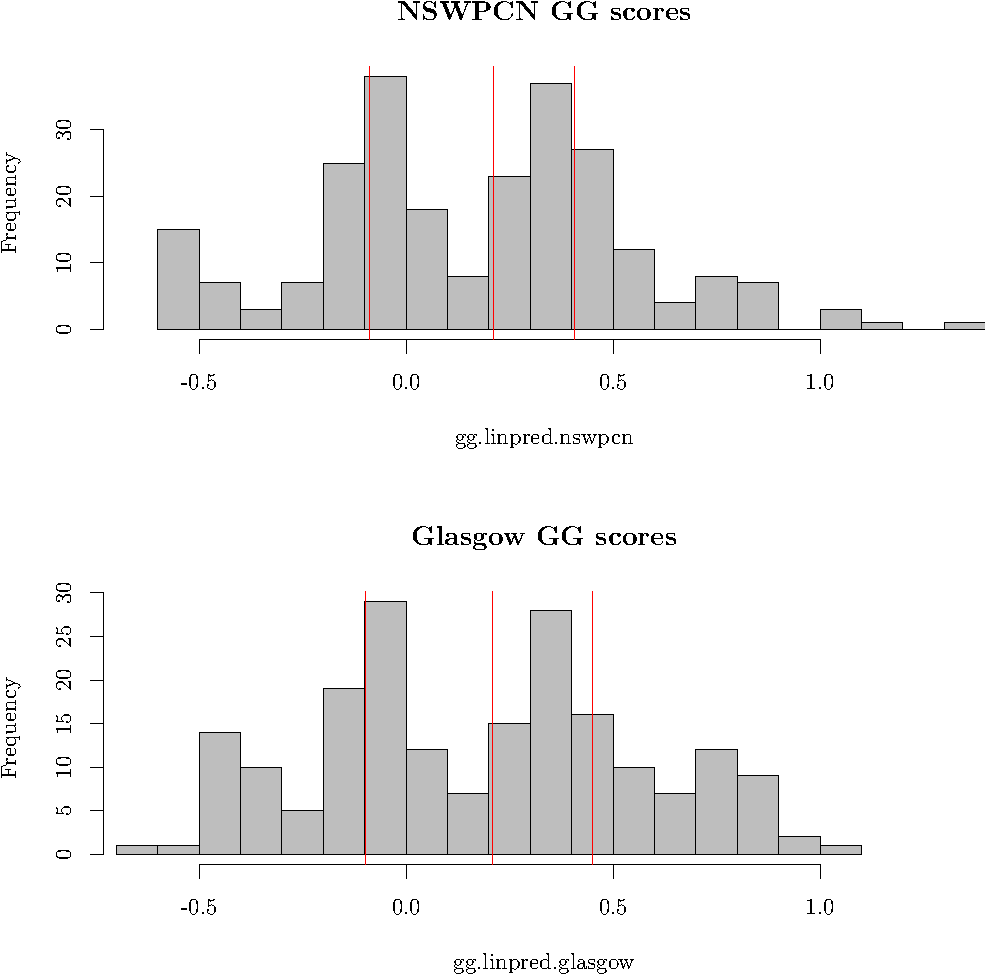
\includegraphics[width=\maxwidth]{figure/05-score-hists-1} 

}


\begin{kframe}\begin{alltt}
\hlkwd{par}\hlstd{(}\hlkwc{mfrow} \hlstd{=} \hlkwd{c}\hlstd{(}\hlnum{1}\hlstd{,} \hlnum{1}\hlstd{))}

\hlkwd{par}\hlstd{(}\hlkwc{mfrow} \hlstd{=} \hlkwd{c}\hlstd{(}\hlnum{2}\hlstd{,} \hlnum{1}\hlstd{))}
\hlkwd{hist}\hlstd{(cph.linpred.nswpcn,} \hlkwc{main} \hlstd{=} \hlstr{"NSWPCN CPH scores"}\hlstd{,} \hlkwc{xlim} \hlstd{=} \hlkwd{range}\hlstd{(}\hlkwd{c}\hlstd{(cph.linpred.nswpcn, cph.linpred.glasgow)),} \hlkwc{breaks} \hlstd{=} \hlnum{20}\hlstd{,} \hlkwc{col} \hlstd{=} \hlstr{"grey"}\hlstd{)}
\hlkwd{abline}\hlstd{(}\hlkwc{v} \hlstd{=} \hlkwd{quantile}\hlstd{(gg.linpred.nswpcn,} \hlkwc{probs} \hlstd{=} \hlkwd{c}\hlstd{(}\hlnum{0.25}\hlstd{,} \hlnum{0.5}\hlstd{,} \hlnum{0.75}\hlstd{)),} \hlkwc{col} \hlstd{=} \hlstr{"red"}\hlstd{)}
\hlkwd{hist}\hlstd{(cph.linpred.glasgow,} \hlkwc{main} \hlstd{=} \hlstr{"Glasgow CPH scores"}\hlstd{,} \hlkwc{xlim} \hlstd{=} \hlkwd{range}\hlstd{(}\hlkwd{c}\hlstd{(cph.linpred.nswpcn, cph.linpred.glasgow)),} \hlkwc{breaks} \hlstd{=} \hlnum{20}\hlstd{,} \hlkwc{col} \hlstd{=} \hlstr{"grey"}\hlstd{)}
\hlkwd{abline}\hlstd{(}\hlkwc{v} \hlstd{=} \hlkwd{quantile}\hlstd{(gg.linpred.glasgow,} \hlkwc{probs} \hlstd{=} \hlkwd{c}\hlstd{(}\hlnum{0.25}\hlstd{,} \hlnum{0.5}\hlstd{,} \hlnum{0.75}\hlstd{)),} \hlkwc{col} \hlstd{=} \hlstr{"red"}\hlstd{)}
\end{alltt}
\end{kframe}

{\centering 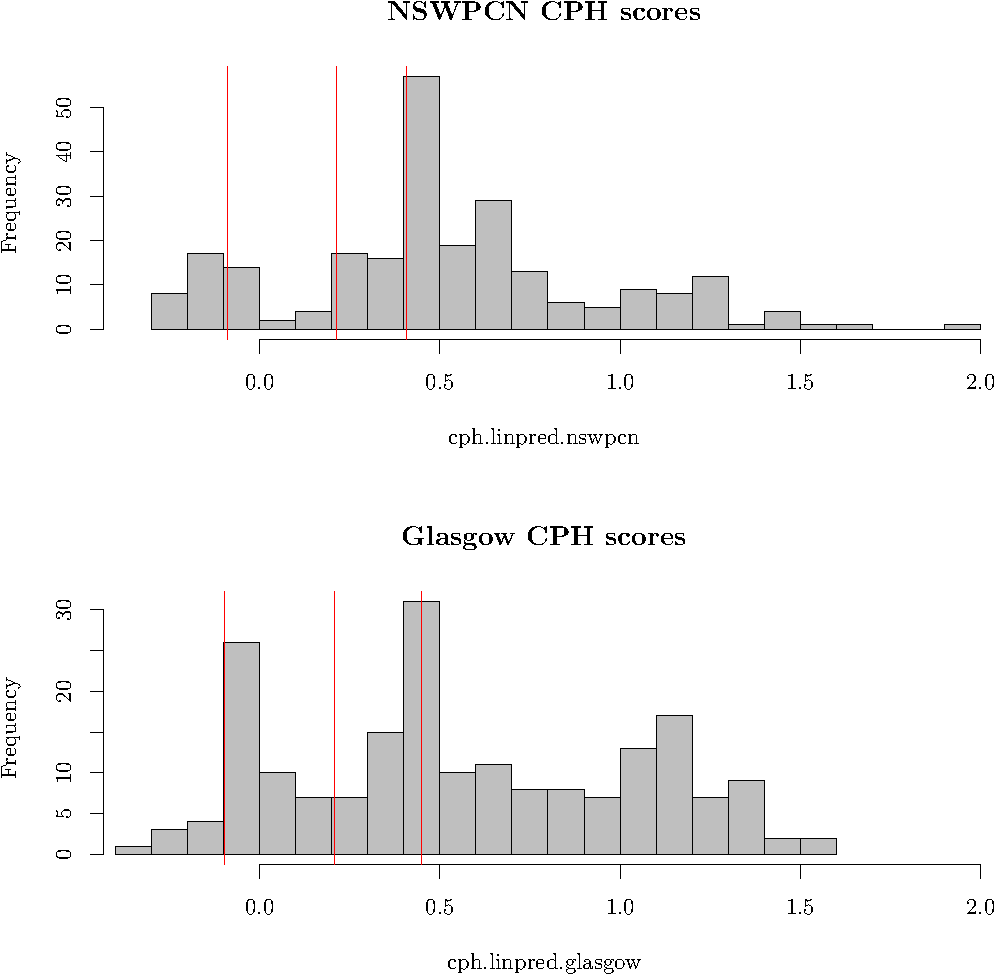
\includegraphics[width=\maxwidth]{figure/05-score-hists-2} 

}


\begin{kframe}\begin{alltt}
\hlkwd{par}\hlstd{(}\hlkwc{mfrow} \hlstd{=} \hlkwd{c}\hlstd{(}\hlnum{1}\hlstd{,} \hlnum{1}\hlstd{))}

\hlkwd{par}\hlstd{(}\hlkwc{mfrow} \hlstd{=} \hlkwd{c}\hlstd{(}\hlnum{2}\hlstd{,} \hlnum{1}\hlstd{))}
\hlkwd{hist}\hlstd{(rsf.linpred.nswpcn,} \hlkwc{main} \hlstd{=} \hlstr{"NSWPCN RSF scores"}\hlstd{,} \hlkwc{xlim} \hlstd{=} \hlkwd{range}\hlstd{(}\hlkwd{c}\hlstd{(rsf.linpred.nswpcn, rsf.linpred.glasgow)),} \hlkwc{breaks} \hlstd{=} \hlnum{20}\hlstd{,} \hlkwc{col} \hlstd{=} \hlstr{"grey"}\hlstd{)}
\hlkwd{abline}\hlstd{(}\hlkwc{v} \hlstd{=} \hlkwd{quantile}\hlstd{(rsf.linpred.nswpcn,} \hlkwc{probs} \hlstd{=} \hlkwd{c}\hlstd{(}\hlnum{0.25}\hlstd{,} \hlnum{0.5}\hlstd{,} \hlnum{0.75}\hlstd{)),} \hlkwc{col} \hlstd{=} \hlstr{"red"}\hlstd{)}
\hlkwd{hist}\hlstd{(rsf.linpred.glasgow,} \hlkwc{main} \hlstd{=} \hlstr{"Glasgow RSF scores"}\hlstd{,} \hlkwc{xlim} \hlstd{=} \hlkwd{range}\hlstd{(}\hlkwd{c}\hlstd{(rsf.linpred.nswpcn, rsf.linpred.glasgow)),} \hlkwc{breaks} \hlstd{=} \hlnum{20}\hlstd{,} \hlkwc{col} \hlstd{=} \hlstr{"grey"}\hlstd{)}
\hlkwd{abline}\hlstd{(}\hlkwc{v} \hlstd{=} \hlkwd{quantile}\hlstd{(rsf.linpred.glasgow,} \hlkwc{probs} \hlstd{=} \hlkwd{c}\hlstd{(}\hlnum{0.25}\hlstd{,} \hlnum{0.5}\hlstd{,} \hlnum{0.75}\hlstd{)),} \hlkwc{col} \hlstd{=} \hlstr{"red"}\hlstd{)}
\end{alltt}
\end{kframe}

{\centering 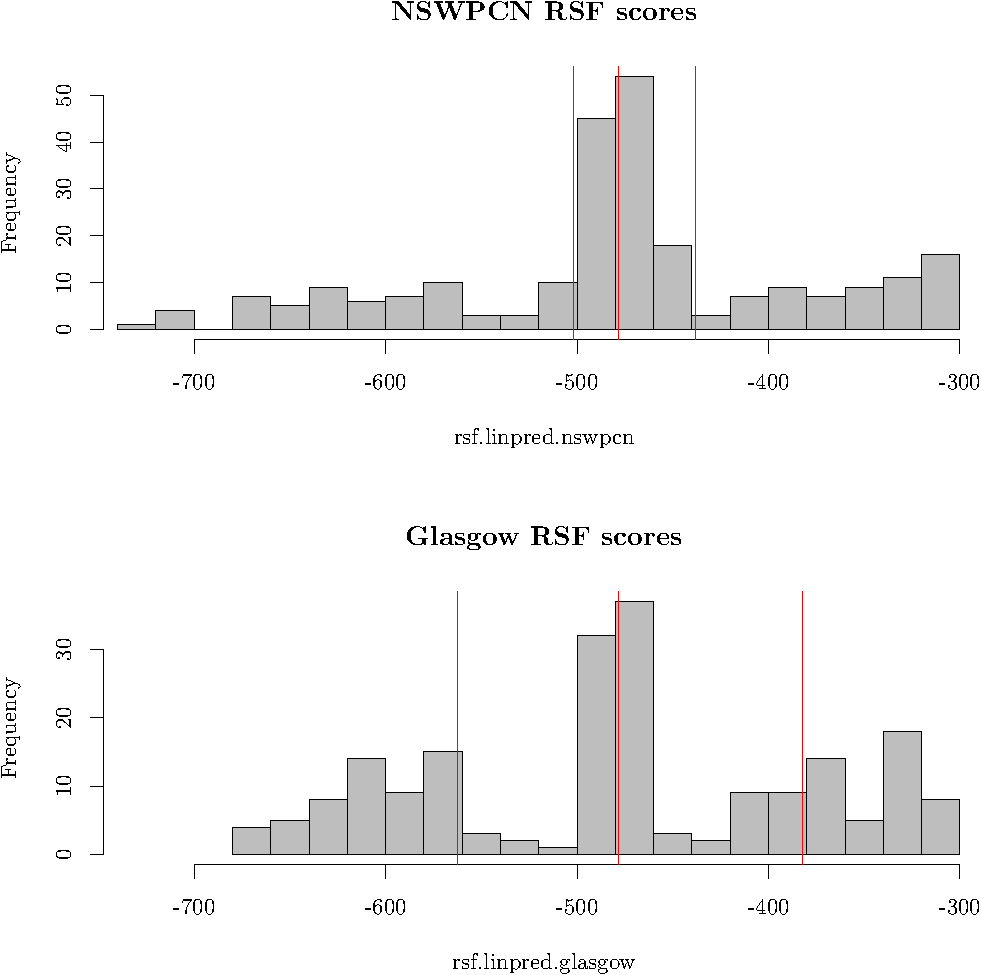
\includegraphics[width=\maxwidth]{figure/05-score-hists-3} 

}


\begin{kframe}\begin{alltt}
\hlkwd{par}\hlstd{(}\hlkwc{mfrow} \hlstd{=} \hlkwd{c}\hlstd{(}\hlnum{1}\hlstd{,} \hlnum{1}\hlstd{))}
\end{alltt}
\end{kframe}
\end{knitrout}

\subsection{Altman method 1 (D,F)}
\begin{knitrout}
\definecolor{shadecolor}{rgb}{0.969, 0.969, 0.969}\color{fgcolor}\begin{kframe}
\begin{alltt}
\hlkwd{summary}\hlstd{(}\hlkwd{coxph}\hlstd{(}\hlkwd{Surv}\hlstd{(Time, DSD)} \hlopt{~} \hlstd{mskcc_post.linpred.glasgow, data.glasgow))}
\end{alltt}
\begin{verbatim}
## Call:
## coxph(formula = Surv(Time, DSD) ~ mskcc_post.linpred.glasgow, 
##     data = data.glasgow)
## 
##   n= 198, number of events= 170 
## 
##                               coef exp(coef) se(coef)    z Pr(>|z|)
## mskcc_post.linpred.glasgow 0.01484   1.01495  0.00405 3.67  0.00025
## 
##                            exp(coef) exp(-coef) lower .95 upper .95
## mskcc_post.linpred.glasgow      1.01      0.985      1.01      1.02
## 
## Concordance= 0.576  (se = 0.025 )
## Rsquare= 0.067   (max possible= 0.999 )
## Likelihood ratio test= 13.6  on 1 df,   p=0.000221
## Wald test            = 13.4  on 1 df,   p=0.000245
## Score (logrank) test = 13.6  on 1 df,   p=0.000229
\end{verbatim}
\begin{alltt}
\hlkwd{summary}\hlstd{(}\hlkwd{coxph}\hlstd{(}\hlkwd{Surv}\hlstd{(Time, DSD)} \hlopt{~} \hlstd{mskcc_pre.linpred.glasgow, data.glasgow))}
\end{alltt}
\begin{verbatim}
## Call:
## coxph(formula = Surv(Time, DSD) ~ mskcc_pre.linpred.glasgow, 
##     data = data.glasgow)
## 
##   n= 198, number of events= 170 
## 
##                                coef exp(coef)  se(coef)     z Pr(>|z|)
## mskcc_pre.linpred.glasgow -0.000423  0.999577  0.007318 -0.06     0.95
## 
##                           exp(coef) exp(-coef) lower .95 upper .95
## mskcc_pre.linpred.glasgow         1          1     0.985      1.01
## 
## Concordance= 0.421  (se = 0.025 )
## Rsquare= 0   (max possible= 0.999 )
## Likelihood ratio test= 0  on 1 df,   p=0.954
## Wald test            = 0  on 1 df,   p=0.954
## Score (logrank) test = 0  on 1 df,   p=0.954
\end{verbatim}
\begin{alltt}
\hlkwd{summary}\hlstd{(}\hlkwd{coxph}\hlstd{(}\hlkwd{Surv}\hlstd{(Time, DSD)} \hlopt{~} \hlstd{gg.linpred.glasgow, data.glasgow))}
\end{alltt}
\begin{verbatim}
## Call:
## coxph(formula = Surv(Time, DSD) ~ gg.linpred.glasgow, data = data.glasgow)
## 
##   n= 198, number of events= 170 
## 
##                     coef exp(coef) se(coef)   z Pr(>|z|)
## gg.linpred.glasgow 0.730     2.076    0.192 3.8  0.00014
## 
##                    exp(coef) exp(-coef) lower .95 upper .95
## gg.linpred.glasgow      2.08      0.482      1.42      3.03
## 
## Concordance= 0.611  (se = 0.025 )
## Rsquare= 0.07   (max possible= 0.999 )
## Likelihood ratio test= 14.4  on 1 df,   p=0.000149
## Wald test            = 14.4  on 1 df,   p=0.000144
## Score (logrank) test = 14.6  on 1 df,   p=0.000131
\end{verbatim}
\begin{alltt}
\hlkwd{summary}\hlstd{(}\hlkwd{coxph}\hlstd{(}\hlkwd{Surv}\hlstd{(Time, DSD)} \hlopt{~} \hlstd{cph.linpred.glasgow, data.glasgow))}
\end{alltt}
\begin{verbatim}
## Call:
## coxph(formula = Surv(Time, DSD) ~ cph.linpred.glasgow, data = data.glasgow)
## 
##   n= 198, number of events= 170 
## 
##                      coef exp(coef) se(coef)    z Pr(>|z|)
## cph.linpred.glasgow 0.853     2.347    0.150 5.68  1.4e-08
## 
##                     exp(coef) exp(-coef) lower .95 upper .95
## cph.linpred.glasgow      2.35      0.426      1.75      3.15
## 
## Concordance= 0.657  (se = 0.025 )
## Rsquare= 0.145   (max possible= 0.999 )
## Likelihood ratio test= 31  on 1 df,   p=2.63e-08
## Wald test            = 32.2  on 1 df,   p=1.37e-08
## Score (logrank) test = 33.5  on 1 df,   p=7.15e-09
\end{verbatim}
\begin{alltt}
\hlkwd{summary}\hlstd{(}\hlkwd{coxph}\hlstd{(}\hlkwd{Surv}\hlstd{(Time, DSD)} \hlopt{~} \hlstd{rsf.linpred.glasgow, data.glasgow))}
\end{alltt}
\begin{verbatim}
## Call:
## coxph(formula = Surv(Time, DSD) ~ rsf.linpred.glasgow, data = data.glasgow)
## 
##   n= 198, number of events= 170 
## 
##                         coef exp(coef) se(coef)    z Pr(>|z|)
## rsf.linpred.glasgow 0.003223  1.003228 0.000807 3.99  6.5e-05
## 
##                     exp(coef) exp(-coef) lower .95 upper .95
## rsf.linpred.glasgow         1      0.997         1         1
## 
## Concordance= 0.614  (se = 0.025 )
## Rsquare= 0.078   (max possible= 0.999 )
## Likelihood ratio test= 16  on 1 df,   p=6.36e-05
## Wald test            = 15.9  on 1 df,   p=6.55e-05
## Score (logrank) test = 16.2  on 1 df,   p=5.8e-05
\end{verbatim}
\begin{alltt}
\hlkwd{anova}\hlstd{(}\hlkwd{coxph}\hlstd{(}\hlkwd{Surv}\hlstd{(Time, DSD)} \hlopt{~} \hlkwd{offset}\hlstd{(gg.linpred.glasgow)} \hlopt{+} \hlstd{gg.linpred.glasgow, data.glasgow))}
\end{alltt}
\begin{verbatim}
## Analysis of Deviance Table
##  Cox model: response is Surv(Time, DSD)
## Terms added sequentially (first to last)
## 
##                    loglik Chisq Df Pr(>|Chi|)
## NULL                 -723                    
## gg.linpred.glasgow   -722  1.97  1       0.16
\end{verbatim}
\begin{alltt}
\hlkwd{anova}\hlstd{(}\hlkwd{coxph}\hlstd{(}\hlkwd{Surv}\hlstd{(Time, DSD)} \hlopt{~} \hlkwd{offset}\hlstd{(cph.linpred.glasgow)} \hlopt{+} \hlstd{cph.linpred.glasgow, data.glasgow))}
\end{alltt}
\begin{verbatim}
## Analysis of Deviance Table
##  Cox model: response is Surv(Time, DSD)
## Terms added sequentially (first to last)
## 
##                     loglik Chisq Df Pr(>|Chi|)
## NULL                  -714                    
## cph.linpred.glasgow   -714  0.96  1       0.33
\end{verbatim}
\begin{alltt}
\hlkwd{anova}\hlstd{(}\hlkwd{coxph}\hlstd{(}\hlkwd{Surv}\hlstd{(Time, DSD)} \hlopt{~} \hlkwd{offset}\hlstd{(rsf.linpred.glasgow)} \hlopt{+} \hlstd{rsf.linpred.glasgow, data.glasgow))}
\end{alltt}


{\ttfamily\noindent\color{warningcolor}{\#\# Warning in fitter(X, Y, strats, offset, init, control, weights = weights, : Ran out of iterations and did not converge}}

{\ttfamily\noindent\bfseries\color{errorcolor}{\#\# Error in fitter(X, Y, strats, offset, init, control, weights = weights, : NA/NaN/Inf in foreign function call (arg 6)}}\end{kframe}
\end{knitrout}
Booyah.


\subsection{Altman method 2 (F)}
\begin{knitrout}
\definecolor{shadecolor}{rgb}{0.969, 0.969, 0.969}\color{fgcolor}\begin{kframe}
\begin{alltt}
\hlkwd{summary}\hlstd{(}\hlkwd{coxph}\hlstd{(}\hlkwd{Surv}\hlstd{(Time, DSD)} \hlopt{~} \hlkwd{offset}\hlstd{(mskcc_pre.linpred.glasgow)} \hlopt{+} \hlstd{AgeCent} \hlopt{+} \hlstd{SexM} \hlopt{+} \hlstd{SizeCent} \hlopt{+} \hlstd{A2} \hlopt{+} \hlstd{A4, data.glasgow))}
\end{alltt}


{\ttfamily\noindent\color{warningcolor}{\#\# Warning in fitter(X, Y, strats, offset, init, control, weights = weights, : Ran out of iterations and did not converge}}

{\ttfamily\noindent\bfseries\color{errorcolor}{\#\# Error in fitter(X, Y, strats, offset, init, control, weights = weights, : NA/NaN/Inf in foreign function call (arg 6)}}\begin{alltt}
\hlkwd{summary}\hlstd{(}\hlkwd{coxph}\hlstd{(}\hlkwd{Surv}\hlstd{(Time, DSD)} \hlopt{~} \hlkwd{offset}\hlstd{(mskcc_post.linpred.glasgow)} \hlopt{+} \hlstd{AgeCent} \hlopt{+} \hlstd{SexM} \hlopt{+} \hlstd{SizeCent} \hlopt{+} \hlstd{A2} \hlopt{+} \hlstd{A4, data.glasgow))}
\end{alltt}
\begin{verbatim}
## Call:
## coxph(formula = Surv(Time, DSD) ~ offset(mskcc_post.linpred.glasgow) + 
##     AgeCent + SexM + SizeCent + A2 + A4, data = data.glasgow)
## 
##   n= 198, number of events= 170 
## 
##               coef exp(coef)  se(coef)      z Pr(>|z|)
## AgeCent    0.22831   1.25648   0.01006  22.69  < 2e-16
## SexMTRUE  -5.22725   0.00537   0.30189 -17.32  < 2e-16
## SizeCent   0.14973   1.16152   0.01910   7.84  4.6e-15
## A2TRUE    -2.29883   0.10038   0.37880  -6.07  1.3e-09
## A4TRUE     4.93307 138.80556   0.29941  16.48  < 2e-16
## 
##          exp(coef) exp(-coef) lower .95 upper .95
## AgeCent   1.26e+00     0.7959   1.23194    1.2815
## SexMTRUE  5.37e-03   186.2805   0.00297    0.0097
## SizeCent  1.16e+00     0.8609   1.11884    1.2058
## A2TRUE    1.00e-01     9.9625   0.04777    0.2109
## A4TRUE    1.39e+02     0.0072  77.18720  249.6137
## 
## Concordance= 0.587  (se = 0.025 )
## Rsquare= 1   (max possible= 1 )
## Likelihood ratio test= 1719  on 5 df,   p=0
## Wald test            = 2210  on 5 df,   p=0
## Score (logrank) test = 12193  on 5 df,   p=0
\end{verbatim}
\begin{alltt}
\hlkwd{summary}\hlstd{(}\hlkwd{coxph}\hlstd{(}\hlkwd{Surv}\hlstd{(Time, DSD)} \hlopt{~} \hlkwd{offset}\hlstd{(gg.linpred.glasgow)} \hlopt{+} \hlstd{AgeCent} \hlopt{+} \hlstd{SexM} \hlopt{+} \hlstd{SizeCent} \hlopt{+} \hlstd{A2} \hlopt{+} \hlstd{A4, data.glasgow))}
\end{alltt}
\begin{verbatim}
## Call:
## coxph(formula = Surv(Time, DSD) ~ offset(gg.linpred.glasgow) + 
##     AgeCent + SexM + SizeCent + A2 + A4, data = data.glasgow)
## 
##   n= 198, number of events= 170 
## 
##              coef exp(coef) se(coef)     z Pr(>|z|)
## AgeCent  -0.03255   0.96797  0.00860 -3.78  0.00015
## SexMTRUE  0.68806   1.98986  0.16160  4.26  2.1e-05
## SizeCent  0.02286   1.02312  0.00737  3.10  0.00194
## A2TRUE    0.21044   1.23422  0.17387  1.21  0.22615
## A4TRUE   -0.06252   0.93940  0.17723 -0.35  0.72427
## 
##          exp(coef) exp(-coef) lower .95 upper .95
## AgeCent      0.968      1.033     0.952     0.984
## SexMTRUE     1.990      0.503     1.450     2.731
## SizeCent     1.023      0.977     1.008     1.038
## A2TRUE       1.234      0.810     0.878     1.735
## A4TRUE       0.939      1.065     0.664     1.330
## 
## Concordance= 0.681  (se = 0.025 )
## Rsquare= 0.196   (max possible= 0.999 )
## Likelihood ratio test= 43.3  on 5 df,   p=3.23e-08
## Wald test            = 44.2  on 5 df,   p=2.13e-08
## Score (logrank) test = 46.1  on 5 df,   p=8.77e-09
\end{verbatim}
\begin{alltt}
\hlkwd{summary}\hlstd{(}\hlkwd{coxph}\hlstd{(}\hlkwd{Surv}\hlstd{(Time, DSD)} \hlopt{~} \hlkwd{offset}\hlstd{(cph.linpred.glasgow)} \hlopt{+} \hlstd{AgeCent} \hlopt{+} \hlstd{SexM} \hlopt{+} \hlstd{SizeCent} \hlopt{+} \hlstd{A2} \hlopt{+} \hlstd{A4, data.glasgow))}
\end{alltt}
\begin{verbatim}
## Call:
## coxph(formula = Surv(Time, DSD) ~ offset(cph.linpred.glasgow) + 
##     AgeCent + SexM + SizeCent + A2 + A4, data = data.glasgow)
## 
##   n= 198, number of events= 170 
## 
##              coef exp(coef) se(coef)     z Pr(>|z|)
## AgeCent  -0.03255   0.96797  0.00860 -3.78  0.00015
## SexMTRUE  0.26736   1.30651  0.16160  1.65  0.09803
## SizeCent  0.01997   1.02017  0.00737  2.71  0.00677
## A2TRUE   -0.10278   0.90232  0.17387 -0.59  0.55443
## A4TRUE   -0.12400   0.88338  0.17723 -0.70  0.48414
## 
##          exp(coef) exp(-coef) lower .95 upper .95
## AgeCent      0.968      1.033     0.952     0.984
## SexMTRUE     1.307      0.765     0.952     1.793
## SizeCent     1.020      0.980     1.006     1.035
## A2TRUE       0.902      1.108     0.642     1.269
## A4TRUE       0.883      1.132     0.624     1.250
## 
## Concordance= 0.681  (se = 0.025 )
## Rsquare= 0.122   (max possible= 0.999 )
## Likelihood ratio test= 25.7  on 5 df,   p=0.000102
## Wald test            = 26.9  on 5 df,   p=5.89e-05
## Score (logrank) test = 27.4  on 5 df,   p=4.78e-05
\end{verbatim}
\begin{alltt}
\hlkwd{summary}\hlstd{(}\hlkwd{coxph}\hlstd{(}\hlkwd{Surv}\hlstd{(Time, DSD)} \hlopt{~} \hlkwd{offset}\hlstd{(rsf.linpred.glasgow)} \hlopt{+} \hlstd{AgeCent} \hlopt{+} \hlstd{SexM} \hlopt{+} \hlstd{SizeCent} \hlopt{+} \hlstd{A2} \hlopt{+} \hlstd{A4, data.glasgow))}
\end{alltt}


{\ttfamily\noindent\color{warningcolor}{\#\# Warning in fitter(X, Y, strats, offset, init, control, weights = weights, : Ran out of iterations and did not converge}}

{\ttfamily\noindent\bfseries\color{errorcolor}{\#\# Error in fitter(X, Y, strats, offset, init, control, weights = weights, : NA/NaN/Inf in foreign function call (arg 6)}}\end{kframe}
\end{knitrout}
Still strong evidence of misspecification or poor fit.  However, the above calibration slope was not significantly different from 1.  Hmm.  This doesn't necessarily sink the method, but will need checking as we go along.

\subsection{Altman method 3 (D)}
Look at the CIs above.

\subsection{Altman method 4 (D,C)}
\begin{knitrout}
\definecolor{shadecolor}{rgb}{0.969, 0.969, 0.969}\color{fgcolor}\begin{kframe}
\begin{alltt}
\hlstd{group_quantiles} \hlkwb{=} \hlkwd{c}\hlstd{(}\hlnum{0}\hlstd{,} \hlnum{0.25}\hlstd{,} \hlnum{0.5}\hlstd{,} \hlnum{0.75}\hlstd{,} \hlnum{1}\hlstd{)}
\hlstd{mskcc_pre.groups.glasgow} \hlkwb{=} \hlkwd{cut}\hlstd{(mskcc_pre.linpred.glasgow,} \hlkwd{quantile}\hlstd{(mskcc_pre.linpred.glasgow, group_quantiles))}
\hlstd{mskcc_post.groups.glasgow} \hlkwb{=} \hlkwd{cut}\hlstd{(mskcc_post.linpred.glasgow,} \hlkwd{quantile}\hlstd{(mskcc_post.linpred.glasgow, group_quantiles))}
\hlstd{gg.groups.glasgow} \hlkwb{=} \hlkwd{cut}\hlstd{(gg.linpred.glasgow,} \hlkwd{quantile}\hlstd{(gg.linpred.glasgow, group_quantiles))}
\hlstd{gg.groups.nswpcn} \hlkwb{=} \hlkwd{cut}\hlstd{(gg.linpred.nswpcn,} \hlkwd{quantile}\hlstd{(gg.linpred.nswpcn, group_quantiles))}
\hlstd{cph.groups.glasgow} \hlkwb{=} \hlkwd{cut}\hlstd{(cph.linpred.glasgow,} \hlkwd{quantile}\hlstd{(cph.linpred.glasgow, group_quantiles))}
\hlstd{cph.groups.nswpcn} \hlkwb{=} \hlkwd{cut}\hlstd{(cph.linpred.nswpcn,} \hlkwd{quantile}\hlstd{(cph.linpred.nswpcn, group_quantiles))}
\hlstd{rsf.groups.glasgow} \hlkwb{=} \hlkwd{cut}\hlstd{(rsf.linpred.glasgow,} \hlkwd{quantile}\hlstd{(rsf.linpred.glasgow, group_quantiles))}
\hlstd{rsf.groups.nswpcn} \hlkwb{=} \hlkwd{cut}\hlstd{(rsf.linpred.nswpcn,} \hlkwd{quantile}\hlstd{(rsf.linpred.nswpcn, group_quantiles))}

\hlkwd{par}\hlstd{(}\hlkwc{mfrow} \hlstd{=} \hlkwd{c}\hlstd{(}\hlnum{2}\hlstd{,} \hlnum{2}\hlstd{))}
\hlkwd{plot}\hlstd{(}\hlkwd{survfit}\hlstd{(}\hlkwd{Surv}\hlstd{(data.nswpcn}\hlopt{$}\hlstd{Time, data.nswpcn}\hlopt{$}\hlstd{DSD)} \hlopt{~} \hlstd{gg.groups.nswpcn),} \hlkwc{col} \hlstd{=} \hlnum{1}\hlopt{:}\hlstd{(}\hlkwd{length}\hlstd{(group_quantiles)}\hlopt{-}\hlnum{1}\hlstd{),} \hlkwc{xlab} \hlstd{=} \hlstr{"Time (days)"}\hlstd{,} \hlkwc{ylab} \hlstd{=} \hlstr{"Fraction Alive"}\hlstd{,} \hlkwc{main} \hlstd{=} \hlstr{"GG: NSWPCN (Resubstitution)"}\hlstd{)}
\hlkwd{plot}\hlstd{(}\hlkwd{survfit}\hlstd{(}\hlkwd{Surv}\hlstd{(data.glasgow}\hlopt{$}\hlstd{Time, data.glasgow}\hlopt{$}\hlstd{DSD)} \hlopt{~} \hlstd{gg.groups.glasgow),} \hlkwc{col} \hlstd{=} \hlnum{1}\hlopt{:}\hlstd{(}\hlkwd{length}\hlstd{(group_quantiles)}\hlopt{-}\hlnum{1}\hlstd{),} \hlkwc{xlab} \hlstd{=} \hlstr{"Time (days)"}\hlstd{,} \hlkwc{ylab} \hlstd{=} \hlstr{"Fraction Alive"}\hlstd{,} \hlkwc{main} \hlstd{=} \hlstr{"GG: Glasgow"}\hlstd{)}
\hlkwd{plot}\hlstd{(}\hlkwd{survfit}\hlstd{(}\hlkwd{Surv}\hlstd{(data.nswpcn}\hlopt{$}\hlstd{Time, data.nswpcn}\hlopt{$}\hlstd{DSD)} \hlopt{~} \hlstd{cph.groups.nswpcn),} \hlkwc{col} \hlstd{=} \hlnum{1}\hlopt{:}\hlstd{(}\hlkwd{length}\hlstd{(group_quantiles)}\hlopt{-}\hlnum{1}\hlstd{),} \hlkwc{xlab} \hlstd{=} \hlstr{"Time (days)"}\hlstd{,} \hlkwc{ylab} \hlstd{=} \hlstr{"Fraction Alive"}\hlstd{,} \hlkwc{main} \hlstd{=} \hlstr{"CPH: NSWPCN (Resubstitution)"}\hlstd{)}
\hlkwd{plot}\hlstd{(}\hlkwd{survfit}\hlstd{(}\hlkwd{Surv}\hlstd{(data.glasgow}\hlopt{$}\hlstd{Time, data.glasgow}\hlopt{$}\hlstd{DSD)} \hlopt{~} \hlstd{cph.groups.glasgow),} \hlkwc{col} \hlstd{=} \hlnum{1}\hlopt{:}\hlstd{(}\hlkwd{length}\hlstd{(group_quantiles)}\hlopt{-}\hlnum{1}\hlstd{),} \hlkwc{xlab} \hlstd{=} \hlstr{"Time (days)"}\hlstd{,} \hlkwc{ylab} \hlstd{=} \hlstr{"Fraction Alive"}\hlstd{,} \hlkwc{main} \hlstd{=} \hlstr{"CPH: Glasgow"}\hlstd{)}
\end{alltt}
\end{kframe}

{\centering 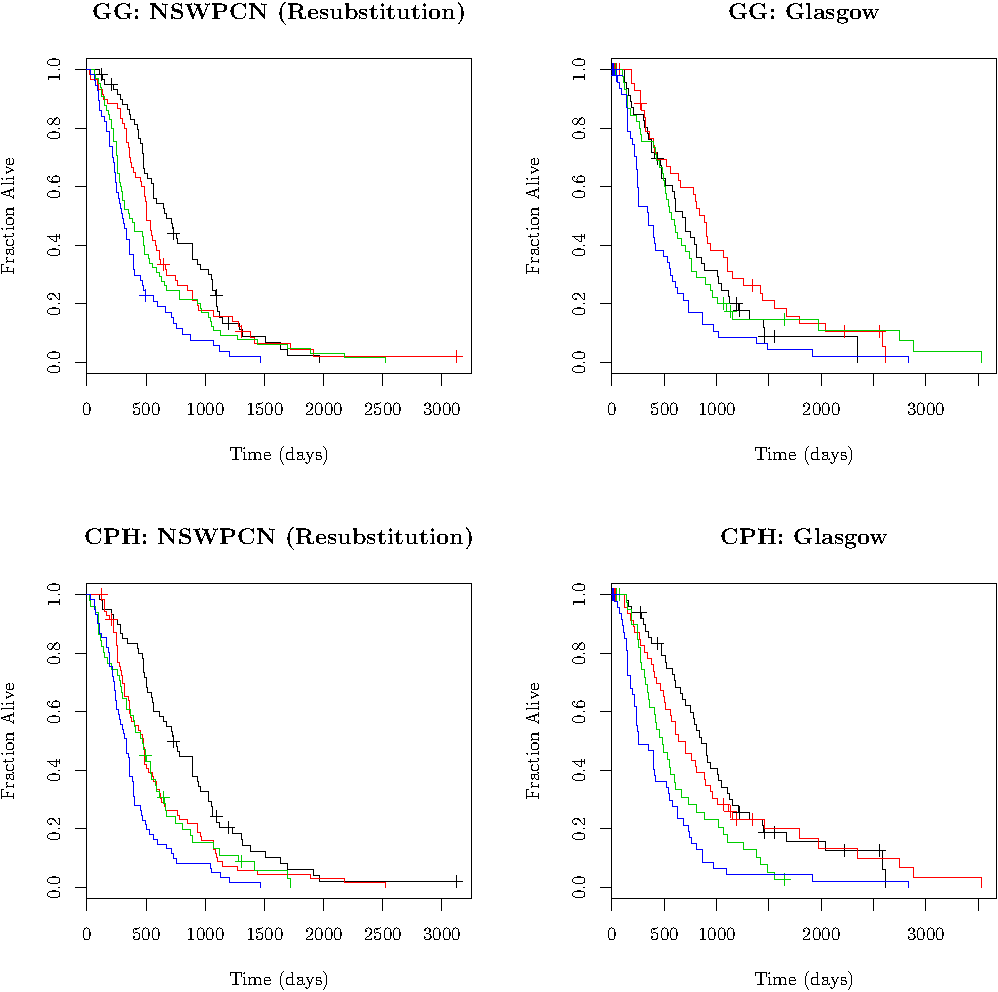
\includegraphics[width=\maxwidth]{figure/05-altman-4-1} 

}


\begin{kframe}\begin{alltt}
\hlkwd{plot}\hlstd{(}\hlkwd{survfit}\hlstd{(}\hlkwd{Surv}\hlstd{(data.nswpcn}\hlopt{$}\hlstd{Time, data.nswpcn}\hlopt{$}\hlstd{DSD)} \hlopt{~} \hlstd{rsf.groups.nswpcn),} \hlkwc{col} \hlstd{=} \hlnum{1}\hlopt{:}\hlstd{(}\hlkwd{length}\hlstd{(group_quantiles)}\hlopt{-}\hlnum{1}\hlstd{),} \hlkwc{xlab} \hlstd{=} \hlstr{"Time (days)"}\hlstd{,} \hlkwc{ylab} \hlstd{=} \hlstr{"Fraction Alive"}\hlstd{,} \hlkwc{main} \hlstd{=} \hlstr{"RSF: NSWPCN (Resubstitution)"}\hlstd{)}
\hlkwd{plot}\hlstd{(}\hlkwd{survfit}\hlstd{(}\hlkwd{Surv}\hlstd{(data.glasgow}\hlopt{$}\hlstd{Time, data.glasgow}\hlopt{$}\hlstd{DSD)} \hlopt{~} \hlstd{rsf.groups.glasgow),} \hlkwc{col} \hlstd{=} \hlnum{1}\hlopt{:}\hlstd{(}\hlkwd{length}\hlstd{(group_quantiles)}\hlopt{-}\hlnum{1}\hlstd{),} \hlkwc{xlab} \hlstd{=} \hlstr{"Time (days)"}\hlstd{,} \hlkwc{ylab} \hlstd{=} \hlstr{"Fraction Alive"}\hlstd{,} \hlkwc{main} \hlstd{=} \hlstr{"RSF: Glasgow"}\hlstd{)}
\hlkwd{plot}\hlstd{(}\hlkwd{survfit}\hlstd{(}\hlkwd{Surv}\hlstd{(data.glasgow}\hlopt{$}\hlstd{Time, data.glasgow}\hlopt{$}\hlstd{DSD)} \hlopt{~} \hlstd{mskcc_pre.groups.glasgow),} \hlkwc{col} \hlstd{=} \hlnum{1}\hlopt{:}\hlstd{(}\hlkwd{length}\hlstd{(group_quantiles)}\hlopt{-}\hlnum{1}\hlstd{),} \hlkwc{xlab} \hlstd{=} \hlstr{"Time (days)"}\hlstd{,} \hlkwc{ylab} \hlstd{=} \hlstr{"Fraction Alive"}\hlstd{,} \hlkwc{main} \hlstd{=} \hlstr{"MSKCC Preop: Glasgow"}\hlstd{)}
\hlkwd{plot}\hlstd{(}\hlkwd{survfit}\hlstd{(}\hlkwd{Surv}\hlstd{(data.glasgow}\hlopt{$}\hlstd{Time, data.glasgow}\hlopt{$}\hlstd{DSD)} \hlopt{~} \hlstd{mskcc_post.groups.glasgow),} \hlkwc{col} \hlstd{=} \hlnum{1}\hlopt{:}\hlstd{(}\hlkwd{length}\hlstd{(group_quantiles)}\hlopt{-}\hlnum{1}\hlstd{),} \hlkwc{xlab} \hlstd{=} \hlstr{"Time (days)"}\hlstd{,} \hlkwc{ylab} \hlstd{=} \hlstr{"Fraction Alive"}\hlstd{,} \hlkwc{main} \hlstd{=} \hlstr{"MSKCC Postop: Glasgow"}\hlstd{)}
\end{alltt}
\end{kframe}

{\centering 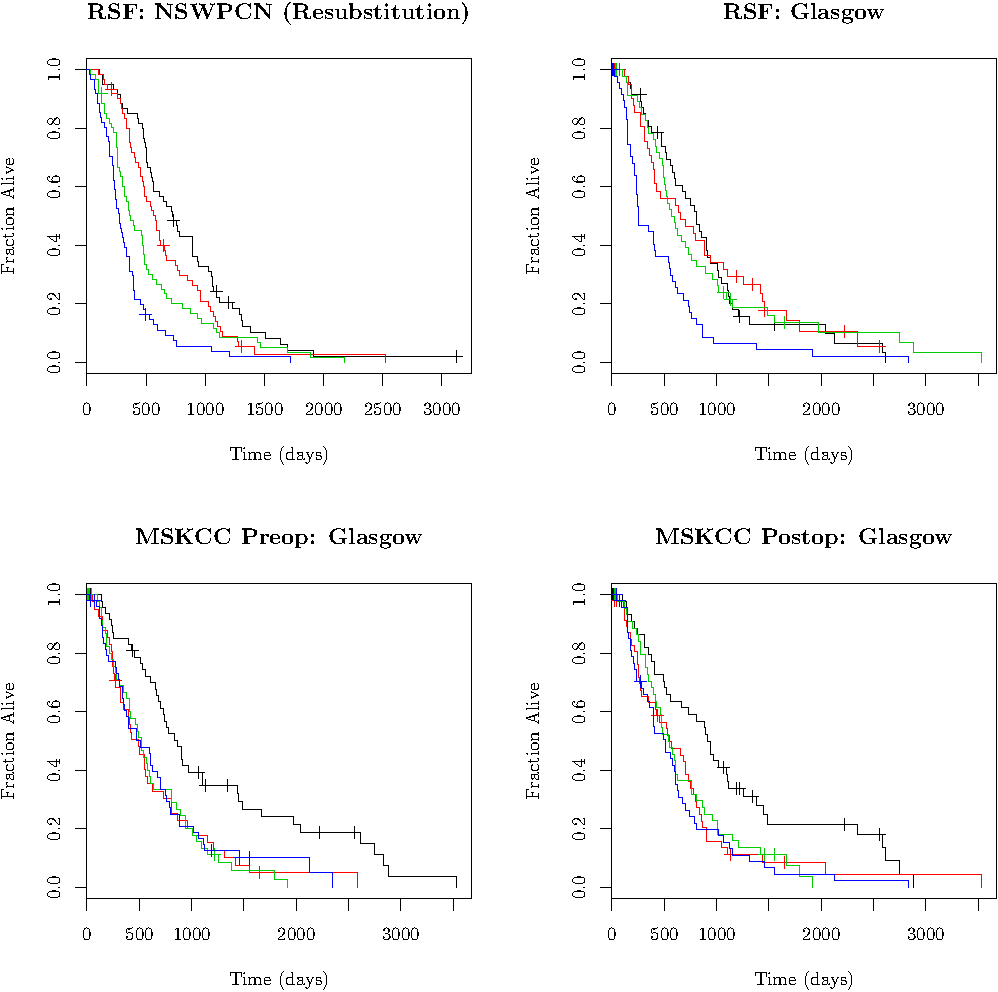
\includegraphics[width=\maxwidth]{figure/05-altman-4-2} 

}


\begin{kframe}\begin{alltt}
\hlkwd{par}\hlstd{(}\hlkwc{mfrow} \hlstd{=} \hlkwd{c}\hlstd{(}\hlnum{1}\hlstd{,} \hlnum{1}\hlstd{))}

\hlcom{# temp = survfit(Surv(data.nswpcn$Time, data.nswpcn$DSD) ~ gg.groups.nswpcn)}
\hlcom{# plot(0 ~ 0, type = "n", xlim = c(0, max(data.nswpcn$Time)), ylim = c(0, 1))}
\hlcom{# for (i in )}
\end{alltt}
\end{kframe}
\end{knitrout}
Weird.  MSKCC somehow is still finding a subgroup, and it's somehow even clearer in preop!  This is based on an approximation to GG only, but should be pretty close.  It certainly does OK on resubstituted data, but not so well on the Glasgow patients.


Decision curve analysis.
\begin{knitrout}
\definecolor{shadecolor}{rgb}{0.969, 0.969, 0.969}\color{fgcolor}\begin{kframe}
\begin{alltt}
\hlstd{temp.data} \hlkwb{=} \hlkwd{data.frame}\hlstd{(}\hlkwc{Time} \hlstd{= data.glasgow}\hlopt{$}\hlstd{Time,} \hlkwc{DSD} \hlstd{= data.glasgow}\hlopt{$}\hlstd{DSD}\hlopt{*}\hlnum{1}\hlstd{,}
    \hlkwc{gg.1} \hlstd{=} \hlnum{1}\hlopt{-}\hlstd{gg.prob.glasgow[val.prob.times} \hlopt{==} \hlnum{365}\hlstd{,],} \hlkwc{gg.2} \hlstd{=} \hlnum{1}\hlopt{-}\hlstd{gg.prob.glasgow[val.prob.times} \hlopt{==} \hlnum{365}\hlopt{*}\hlnum{2}\hlstd{,],} \hlkwc{gg.3} \hlstd{=} \hlnum{1}\hlopt{-}\hlstd{gg.prob.glasgow[val.prob.times} \hlopt{==} \hlnum{365}\hlopt{*}\hlnum{3}\hlstd{,],}
    \hlkwc{gg2.1} \hlstd{=} \hlnum{1}\hlopt{-}\hlstd{gg2.prob.glasgow[val.prob.times} \hlopt{==} \hlnum{365}\hlstd{,],} \hlkwc{gg2.2} \hlstd{=} \hlnum{1}\hlopt{-}\hlstd{gg2.prob.glasgow[val.prob.times} \hlopt{==} \hlnum{365}\hlopt{*}\hlnum{2}\hlstd{,],} \hlkwc{gg2.3} \hlstd{=} \hlnum{1}\hlopt{-}\hlstd{gg2.prob.glasgow[val.prob.times} \hlopt{==} \hlnum{365}\hlopt{*}\hlnum{3}\hlstd{,],}
    \hlkwc{cph.1} \hlstd{=} \hlnum{1}\hlopt{-}\hlstd{cph.prob.glasgow[val.prob.times} \hlopt{==} \hlnum{365}\hlstd{,],} \hlkwc{cph.2} \hlstd{=} \hlnum{1}\hlopt{-}\hlstd{cph.prob.glasgow[val.prob.times} \hlopt{==} \hlnum{365}\hlopt{*}\hlnum{2}\hlstd{,],} \hlkwc{cph.3} \hlstd{=} \hlnum{1}\hlopt{-}\hlstd{cph.prob.glasgow[val.prob.times} \hlopt{==} \hlnum{365}\hlopt{*}\hlnum{3}\hlstd{,],}
    \hlkwc{rsf.1} \hlstd{=} \hlnum{1}\hlopt{-}\hlstd{rsf.prob.glasgow[val.prob.times} \hlopt{==} \hlnum{365}\hlstd{,],} \hlkwc{rsf.2} \hlstd{=} \hlnum{1}\hlopt{-}\hlstd{rsf.prob.glasgow[val.prob.times} \hlopt{==} \hlnum{365}\hlopt{*}\hlnum{2}\hlstd{,],} \hlkwc{rsf.3} \hlstd{=} \hlnum{1}\hlopt{-}\hlstd{rsf.prob.glasgow[val.prob.times} \hlopt{==} \hlnum{365}\hlopt{*}\hlnum{3}\hlstd{,],}
    \hlkwc{mskcc.pre.1} \hlstd{=} \hlnum{1}\hlopt{-}\hlstd{mskcc_pre.12mo.glasgow,} \hlkwc{mskcc.pre.2} \hlstd{=} \hlnum{1}\hlopt{-}\hlstd{mskcc_pre.24mo.glasgow,} \hlkwc{mskcc.pre.3} \hlstd{=} \hlnum{1}\hlopt{-}\hlstd{mskcc_pre.36mo.glasgow,}
    \hlkwc{mskcc.post.1} \hlstd{=} \hlnum{1}\hlopt{-}\hlstd{mskcc_post.12mo.glasgow,} \hlkwc{mskcc.post.2} \hlstd{=} \hlnum{1}\hlopt{-}\hlstd{mskcc_post.24mo.glasgow,} \hlkwc{mskcc.post.3} \hlstd{=} \hlnum{1}\hlopt{-}\hlstd{mskcc_post.36mo.glasgow)}
\hlkwd{stdca}\hlstd{(}\hlkwc{data} \hlstd{= temp.data,} \hlkwc{outcome} \hlstd{=} \hlstr{"DSD"}\hlstd{,} \hlkwc{ttoutcome} \hlstd{=} \hlstr{"Time"}\hlstd{,} \hlkwc{predictors} \hlstd{=} \hlkwd{c}\hlstd{(}\hlstr{"gg.1"}\hlstd{,} \hlstr{"cph.1"}\hlstd{,} \hlstr{"rsf.1"}\hlstd{,} \hlstr{"mskcc.pre.1"}\hlstd{,} \hlstr{"mskcc.post.1"}\hlstd{),} \hlkwc{timepoint} \hlstd{=} \hlnum{365}\hlstd{,} \hlkwc{probability} \hlstd{=} \hlkwd{rep}\hlstd{(}\hlnum{TRUE}\hlstd{,} \hlnum{5}\hlstd{))}
\end{alltt}
\begin{verbatim}
## [1] "gg.1: No observations with risk greater than 69% that have followup through the timepoint selected, and therefore net benefit not calculable in this range."        
## [2] "cph.1: No observations with risk greater than 75% that have followup through the timepoint selected, and therefore net benefit not calculable in this range."       
## [3] "rsf.1: No observations with risk greater than 58% that have followup through the timepoint selected, and therefore net benefit not calculable in this range."       
## [4] "mskcc.pre.1: No observations with risk greater than 44%, and therefore net benefit not calculable in this range."                                                   
## [5] "mskcc.post.1: No observations with risk greater than 31% that have followup through the timepoint selected, and therefore net benefit not calculable in this range."
\end{verbatim}
\end{kframe}

{\centering 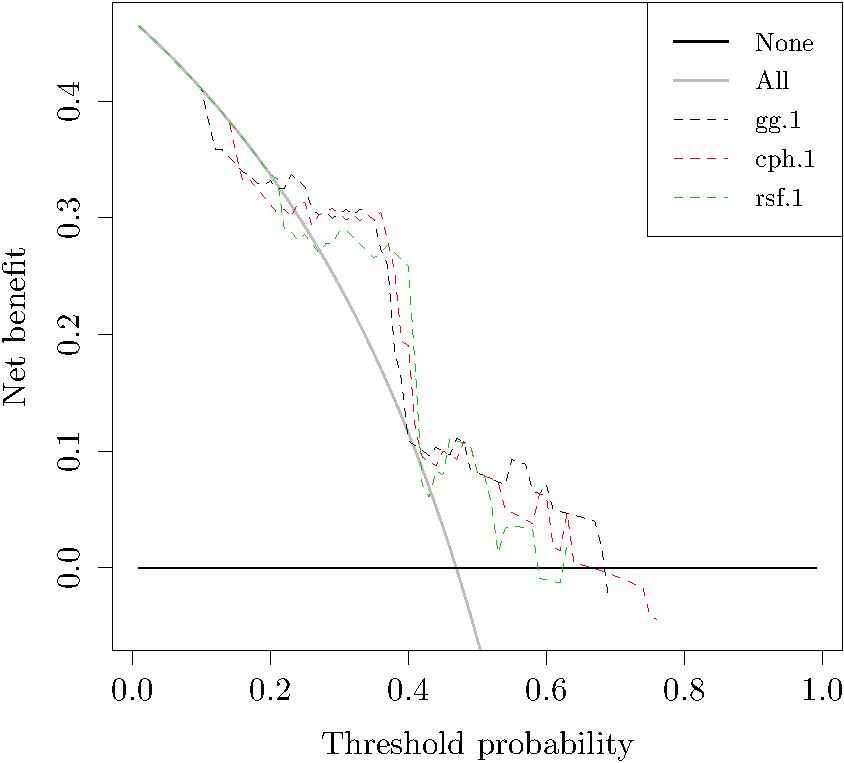
\includegraphics[width=\maxwidth]{figure/05-model-selection-dca-1} 

}


\begin{kframe}\begin{verbatim}
## $N
## [1] 198
## 
## $predictors
##      predictor harm.applied probability
## 1         gg.1            0        TRUE
## 2        cph.1            0        TRUE
## 3        rsf.1            0        TRUE
## 4  mskcc.pre.1            0        TRUE
## 5 mskcc.post.1            0        TRUE
## 
## $interventions.avoided.per
## [1] 100
## 
## $net.benefit
##    threshold        all none       gg.1      cph.1      rsf.1 mskcc.pre.1
## 1       0.01   0.306589    0  3.066e-01  0.3065893  0.3065893    0.306589
## 2       0.02   0.299514    0  2.995e-01  0.2995137  0.2995137    0.299514
## 3       0.03   0.292292    0  2.923e-01  0.2922922  0.2922922    0.292292
## 4       0.04   0.284920    0  2.849e-01  0.2849202  0.2849202    0.284920
## 5       0.05   0.277393    0  2.774e-01  0.2773931  0.2773931    0.277393
## 6       0.06   0.269706    0  2.697e-01  0.2697058  0.2697058    0.269706
## 7       0.07   0.261853    0  2.619e-01  0.2618532  0.2618532    0.261853
## 8       0.08   0.253830    0  2.538e-01  0.2538298  0.2538298    0.253830
## 9       0.09   0.245630    0  2.456e-01  0.2456301  0.2456301    0.245630
## 10      0.10   0.237248    0  2.372e-01  0.2372483  0.2372483    0.237248
## 11      0.11   0.228678    0  2.295e-01  0.2286780  0.2286780    0.228678
## 12      0.12   0.219913    0  2.208e-01  0.2199130  0.2199130    0.219913
## 13      0.13   0.210946    0  2.119e-01  0.2109465  0.2109465    0.210946
## 14      0.14   0.201771    0  2.028e-01  0.2017714  0.2017714    0.201771
## 15      0.15   0.192381    0  1.945e-01  0.1934405  0.1923805    0.192381
## 16      0.16   0.182766    0  1.798e-01  0.1838987  0.1827660    0.189592
## 17      0.17   0.172920    0  1.791e-01  0.1741270  0.1729198    0.186558
## 18      0.18   0.162833    0  1.701e-01  0.1654025  0.1628335    0.181338
## 19      0.19   0.152498    0  1.568e-01  0.1593271  0.1524981    0.082587
## 20      0.20   0.141904    0  1.488e-01  0.1410995  0.1419043    0.005051
## 21      0.21   0.131042    0  1.446e-01  0.1416072  0.1325664    0.002365
## 22      0.22   0.119902    0  1.375e-01  0.1293876  0.1215102    0.002202
## 23      0.23   0.108472    0  1.327e-01  0.1235510  0.1169676    0.002033
## 24      0.24   0.096741    0  1.130e-01  0.1138131  0.1054344    0.001861
## 25      0.25   0.084698    0  1.141e-01  0.1057266  0.1092942    0.001684
## 26      0.26   0.072329    0  1.036e-01  0.0780081  0.0905894    0.001502
## 27      0.27   0.059621    0  9.483e-02  0.0739156  0.0749007   -0.003736
## 28      0.28   0.046560    0  8.667e-02  0.0628975  0.0598748   -0.003928
## 29      0.29   0.033132    0  8.399e-02  0.0660750  0.0629576   -0.004126
## 30      0.30   0.019319    0  7.595e-02  0.0651715  0.0740064   -0.004329
## 31      0.31   0.005106    0  7.587e-02  0.0688417  0.0719203   -0.004538
## 32      0.32  -0.009524    0  6.540e-02  0.0685007  0.0597343    0.005051
## 33      0.33  -0.024592    0  6.047e-02  0.0610051  0.0473221    0.005051
## 34      0.34  -0.040116    0  5.281e-02  0.0523853  0.0498159    0.005051
## 35      0.35  -0.056118    0  4.795e-02  0.0445666  0.0334745    0.005051
## 36      0.36  -0.072620    0  4.857e-02  0.0367386  0.0226912    0.005051
## 37      0.37  -0.089645    0  5.014e-02  0.0288241  0.0182025    0.005051
## 38      0.38  -0.107220    0  4.368e-02  0.0177695  0.0090016    0.005051
## 39      0.39  -0.125371    0  4.830e-02  0.0271126  0.0009429    0.005051
## 40      0.40  -0.144128    0  3.599e-02  0.0197362 -0.0126816    0.005051
## 41      0.41  -0.163520    0  1.855e-02  0.0309890 -0.0174713    0.005051
## 42      0.42  -0.183580    0  3.941e-02  0.0061253 -0.0183568    0.005051
## 43      0.43  -0.204345    0  3.327e-02  0.0278254 -0.0226650    0.005051
## 44      0.44  -0.225851    0  2.581e-02  0.0211855  0.0006950          NA
## 45      0.45  -0.248139    0  1.939e-02  0.0146837  0.0309291          NA
## 46      0.46  -0.271253    0  1.743e-02  0.0071510  0.0389076          NA
## 47      0.47  -0.295239    0  2.486e-02  0.0003295  0.0388449          NA
## 48      0.48  -0.320147    0  1.864e-02  0.0082860  0.0292435          NA
## 49      0.49  -0.346032    0  6.549e-03  0.0013034  0.0193760          NA
## 50      0.50  -0.372953    0 -8.981e-05 -0.0162376  0.0207632          NA
## 51      0.51  -0.400973    0 -1.181e-02 -0.0228177 -0.0031952          NA
## 52      0.52  -0.430160    0 -1.242e-02 -0.0181641 -0.0170004          NA
## 53      0.53  -0.460588    0 -1.902e-02 -0.0249980 -0.0087041          NA
## 54      0.54  -0.492340    0 -1.968e-02 -0.0132078 -0.0118577          NA
## 55      0.55  -0.525503    0 -3.199e-02 -0.0250408 -0.0072952          NA
## 56      0.56  -0.560174    0 -2.527e-02 -0.0172036  0.0027548          NA
## 57      0.57  -0.596457    0 -2.527e-02 -0.0166393  0.0152690          NA
## 58      0.58  -0.634468    0 -3.224e-02 -0.0230479         NA          NA
## 59      0.59  -0.674333    0 -7.076e-03 -0.0046638         NA          NA
## 60      0.60  -0.716191    0 -1.319e-02 -0.0103359         NA          NA
## 61      0.61  -0.760196    0 -1.137e-02 -0.0237749         NA          NA
## 62      0.62  -0.806517    0 -2.840e-02 -0.0297169         NA          NA
## 63      0.63  -0.855342    0  4.489e-03 -0.0359800         NA          NA
## 64      0.64  -0.906879    0  1.569e-02 -0.0490620         NA          NA
## 65      0.65  -0.961362    0  2.170e-02 -0.0609031         NA          NA
## 66      0.66  -1.019049    0  3.330e-02 -0.0583284         NA          NA
## 67      0.67  -1.080232    0  3.094e-02 -0.0543048         NA          NA
## 68      0.68  -1.145239    0  2.320e-02 -0.0710227         NA          NA
## 69      0.69  -1.214441    0         NA -0.0773868         NA          NA
## 70      0.70  -1.288255    0         NA -0.0448934         NA          NA
## 71      0.71  -1.367161    0         NA -0.0548589         NA          NA
## 72      0.72  -1.451702    0         NA -0.0458430         NA          NA
## 73      0.73  -1.542506    0         NA -0.0210183         NA          NA
## 74      0.74  -1.640294    0         NA -0.0299145         NA          NA
## 75      0.75  -1.745906    0         NA         NA         NA          NA
## 76      0.76  -1.860319    0         NA         NA         NA          NA
## 77      0.77  -1.984681    0         NA         NA         NA          NA
## 78      0.78  -2.120348    0         NA         NA         NA          NA
## 79      0.79  -2.268936    0         NA         NA         NA          NA
## 80      0.80  -2.432383    0         NA         NA         NA          NA
## 81      0.81  -2.613035    0         NA         NA         NA          NA
## 82      0.82  -2.813759    0         NA         NA         NA          NA
## 83      0.83  -3.038097    0         NA         NA         NA          NA
## 84      0.84  -3.290479    0         NA         NA         NA          NA
## 85      0.85  -3.576510    0         NA         NA         NA          NA
## 86      0.86  -3.903404    0         NA         NA         NA          NA
## 87      0.87  -4.280589    0         NA         NA         NA          NA
## 88      0.88  -4.720638    0         NA         NA         NA          NA
## 89      0.89  -5.240696    0         NA         NA         NA          NA
## 90      0.90  -5.864766    0         NA         NA         NA          NA
## 91      0.91  -6.627517    0         NA         NA         NA          NA
## 92      0.92  -7.580957    0         NA         NA         NA          NA
## 93      0.93  -8.806808    0         NA         NA         NA          NA
## 94      0.94 -10.441276    0         NA         NA         NA          NA
## 95      0.95 -12.729531    0         NA         NA         NA          NA
## 96      0.96 -16.161914    0         NA         NA         NA          NA
## 97      0.97 -21.882552    0         NA         NA         NA          NA
## 98      0.98 -33.323828    0         NA         NA         NA          NA
## 99      0.99 -67.647657    0         NA         NA         NA          NA
##    mskcc.post.1
## 1      0.306589
## 2      0.299514
## 3      0.292292
## 4      0.284920
## 5      0.277393
## 6      0.269706
## 7      0.261853
## 8      0.253830
## 9      0.245630
## 10     0.237248
## 11     0.229463
## 12     0.225051
## 13     0.206737
## 14     0.200009
## 15     0.195373
## 16     0.179161
## 17     0.150617
## 18     0.110140
## 19     0.108100
## 20     0.080708
## 21     0.074611
## 22     0.048221
## 23     0.033413
## 24     0.014784
## 25     0.003573
## 26     0.016870
## 27     0.015221
## 28     0.015917
## 29     0.013231
## 30     0.010582
## 31           NA
## 32           NA
## 33           NA
## 34           NA
## 35           NA
## 36           NA
## 37           NA
## 38           NA
## 39           NA
## 40           NA
## 41           NA
## 42           NA
## 43           NA
## 44           NA
## 45           NA
## 46           NA
## 47           NA
## 48           NA
## 49           NA
## 50           NA
## 51           NA
## 52           NA
## 53           NA
## 54           NA
## 55           NA
## 56           NA
## 57           NA
## 58           NA
## 59           NA
## 60           NA
## 61           NA
## 62           NA
## 63           NA
## 64           NA
## 65           NA
## 66           NA
## 67           NA
## 68           NA
## 69           NA
## 70           NA
## 71           NA
## 72           NA
## 73           NA
## 74           NA
## 75           NA
## 76           NA
## 77           NA
## 78           NA
## 79           NA
## 80           NA
## 81           NA
## 82           NA
## 83           NA
## 84           NA
## 85           NA
## 86           NA
## 87           NA
## 88           NA
## 89           NA
## 90           NA
## 91           NA
## 92           NA
## 93           NA
## 94           NA
## 95           NA
## 96           NA
## 97           NA
## 98           NA
## 99           NA
## 
## $interventions.avoided
##    threshold    gg.1   cph.1   rsf.1 mskcc.pre.1 mskcc.post.1
## 1       0.01  0.0000  0.0000  0.0000       0.000       0.0000
## 2       0.02  0.0000  0.0000  0.0000       0.000       0.0000
## 3       0.03  0.0000  0.0000  0.0000       0.000       0.0000
## 4       0.04  0.0000  0.0000  0.0000       0.000       0.0000
## 5       0.05  0.0000  0.0000  0.0000       0.000       0.0000
## 6       0.06  0.0000  0.0000  0.0000       0.000       0.0000
## 7       0.07  0.0000  0.0000  0.0000       0.000       0.0000
## 8       0.08  0.0000  0.0000  0.0000       0.000       0.0000
## 9       0.09  0.0000  0.0000  0.0000       0.000       0.0000
## 10      0.10  0.0000  0.0000  0.0000       0.000       0.0000
## 11      0.11  0.6354  0.0000  0.0000       0.000       0.6354
## 12      0.12  0.6246  0.0000  0.0000       0.000       3.7681
## 13      0.13  0.6154  0.0000  0.0000       0.000      -2.8173
## 14      0.14  0.6075  0.0000  0.0000       0.000      -1.0828
## 15      0.15  1.2024  0.6007  0.0000       0.000       1.6956
## 16      0.16 -1.5388  0.5947  0.0000       3.584      -1.8925
## 17      0.17  3.0082  0.5894  0.0000       6.659     -10.8891
## 18      0.18  3.2900  1.1704  0.0000       8.430     -24.0046
## 19      0.19  1.8332  2.9113  0.0000     -29.804     -18.9276
## 20      0.20  2.7580 -0.3219  0.0000     -54.742     -24.4785
## 21      0.21  5.1157  3.9744  0.5733     -48.407     -21.2290
## 22      0.22  6.2283  3.3632  0.5702     -41.730     -25.4140
## 23      0.23  8.1059  5.0482  2.8442     -35.634     -25.1286
## 24      0.24  5.1462  5.4060  2.7528     -30.046     -25.9530
## 25      0.25  8.8213  6.3086  7.3789     -24.904     -24.3376
## 26      0.26  8.8871  1.6164  5.1972     -20.159     -15.7845
## 27      0.27  9.5182  3.8648  4.1311     -17.130     -12.0046
## 28      0.28 10.3147  4.2010  3.4237     -12.983      -7.8798
## 29      0.29 12.4515  8.0655  7.3022      -9.122      -4.8722
## 30      0.30 13.2149 10.6989 12.7603      -5.518      -2.0387
## 31      0.31 15.7504 14.1862 14.8715      -2.147           NA
## 32      0.32 15.9210 16.5803 14.7175       3.097           NA
## 33      0.33 17.2692 17.3788 14.6007       6.018           NA
## 34      0.34 18.0387 17.9561 17.4574       8.768           NA
## 35      0.35 19.3266 18.6985 16.6386      11.360           NA
## 36      0.36 21.5449 19.4415 16.9441      13.808           NA
## 37      0.37 23.8021 20.1718 18.3633      16.124           NA
## 38      0.38 24.6206 20.3931 18.9625      18.318           NA
## 39      0.39 27.1646 23.8501 19.7569      20.399           NA
## 40      0.40 27.0174 24.5796 19.7169      22.377           NA
## 41      0.41 26.2010 27.9903 21.0167      24.258           NA
## 42      0.42 30.7932 26.1974 22.8166      26.049           NA
## 43      0.43 31.4983 30.7761 24.0831      27.757           NA
## 44      0.44 32.0290 31.4410 28.8331          NA           NA
## 45      0.45 32.6978 32.1228 34.1084          NA           NA
## 46      0.46 33.8888 32.6822 36.4101          NA           NA
## 47      0.47 36.0965 33.3300 37.6733          NA           NA
## 48      0.48 36.7018 35.5803 37.8507          NA           NA
## 49      0.49 36.6972 36.1513 38.0323          NA           NA
## 50      0.50 37.2863 35.6715 39.3716          NA           NA
## 51      0.51 37.3905 36.3325 38.2178          NA           NA
## 52      0.52 38.5610 38.0303 38.1378          NA           NA
## 53      0.53 39.1580 38.6278 40.0728          NA           NA
## 54      0.54 40.2634 40.8150 40.9300          NA           NA
## 55      0.55 40.3787 40.9470 42.3989          NA           NA
## 56      0.56 42.0282 42.6620 44.2301          NA           NA
## 57      0.57 43.0898 43.7406 46.1478          NA           NA
## 58      0.58 43.6095 44.2752      NA          NA           NA
## 59      0.59 46.3687 46.5363      NA          NA           NA
## 60      0.60 46.8669 47.0570      NA          NA           NA
## 61      0.61 47.8756 47.0827      NA          NA           NA
## 62      0.62 47.6908 47.6103      NA          NA           NA
## 63      0.63 50.4980 48.1213      NA          NA           NA
## 64      0.64 51.8947 48.2522      NA          NA           NA
## 65      0.65 52.9340 48.4862      NA          NA           NA
## 66      0.66 54.2120 49.4917      NA          NA           NA
## 67      0.67 54.7296 50.5307      NA          NA           NA
## 68      0.68 54.9854 50.5514      NA          NA           NA
## 69      0.69      NA 51.0850      NA          NA           NA
## 70      0.70      NA 53.2869      NA          NA           NA
## 71      0.71      NA 53.6011      NA          NA           NA
## 72      0.72      NA 54.6723      NA          NA           NA
## 73      0.73      NA 56.2742      NA          NA           NA
## 74      0.74      NA 56.5809      NA          NA           NA
## 75      0.75      NA      NA      NA          NA           NA
## 76      0.76      NA      NA      NA          NA           NA
## 77      0.77      NA      NA      NA          NA           NA
## 78      0.78      NA      NA      NA          NA           NA
## 79      0.79      NA      NA      NA          NA           NA
## 80      0.80      NA      NA      NA          NA           NA
## 81      0.81      NA      NA      NA          NA           NA
## 82      0.82      NA      NA      NA          NA           NA
## 83      0.83      NA      NA      NA          NA           NA
## 84      0.84      NA      NA      NA          NA           NA
## 85      0.85      NA      NA      NA          NA           NA
## 86      0.86      NA      NA      NA          NA           NA
## 87      0.87      NA      NA      NA          NA           NA
## 88      0.88      NA      NA      NA          NA           NA
## 89      0.89      NA      NA      NA          NA           NA
## 90      0.90      NA      NA      NA          NA           NA
## 91      0.91      NA      NA      NA          NA           NA
## 92      0.92      NA      NA      NA          NA           NA
## 93      0.93      NA      NA      NA          NA           NA
## 94      0.94      NA      NA      NA          NA           NA
## 95      0.95      NA      NA      NA          NA           NA
## 96      0.96      NA      NA      NA          NA           NA
## 97      0.97      NA      NA      NA          NA           NA
## 98      0.98      NA      NA      NA          NA           NA
## 99      0.99      NA      NA      NA          NA           NA
\end{verbatim}
\begin{alltt}
\hlkwd{stdca}\hlstd{(}\hlkwc{data} \hlstd{= temp.data,} \hlkwc{outcome} \hlstd{=} \hlstr{"DSD"}\hlstd{,} \hlkwc{ttoutcome} \hlstd{=} \hlstr{"Time"}\hlstd{,} \hlkwc{predictors} \hlstd{=} \hlkwd{c}\hlstd{(}\hlstr{"gg.2"}\hlstd{,} \hlstr{"cph.2"}\hlstd{,} \hlstr{"rsf.2"}\hlstd{,} \hlstr{"mskcc.pre.2"}\hlstd{,} \hlstr{"mskcc.post.2"}\hlstd{),} \hlkwc{timepoint} \hlstd{=} \hlnum{365}\hlopt{*}\hlnum{2}\hlstd{,} \hlkwc{probability} \hlstd{=} \hlkwd{rep}\hlstd{(}\hlnum{TRUE}\hlstd{,} \hlnum{5}\hlstd{))}
\end{alltt}
\begin{verbatim}
## [1] "gg.2: No observations with risk greater than 98% that have followup through the timepoint selected, and therefore net benefit not calculable in this range."        
## [2] "cph.2: No observations with risk greater than 98% that have followup through the timepoint selected, and therefore net benefit not calculable in this range."       
## [3] "rsf.2: No observations with risk greater than 89%, and therefore net benefit not calculable in this range."                                                         
## [4] "mskcc.pre.2: No observations with risk greater than 79%, and therefore net benefit not calculable in this range."                                                   
## [5] "mskcc.post.2: No observations with risk greater than 63% that have followup through the timepoint selected, and therefore net benefit not calculable in this range."
\end{verbatim}
\end{kframe}

{\centering 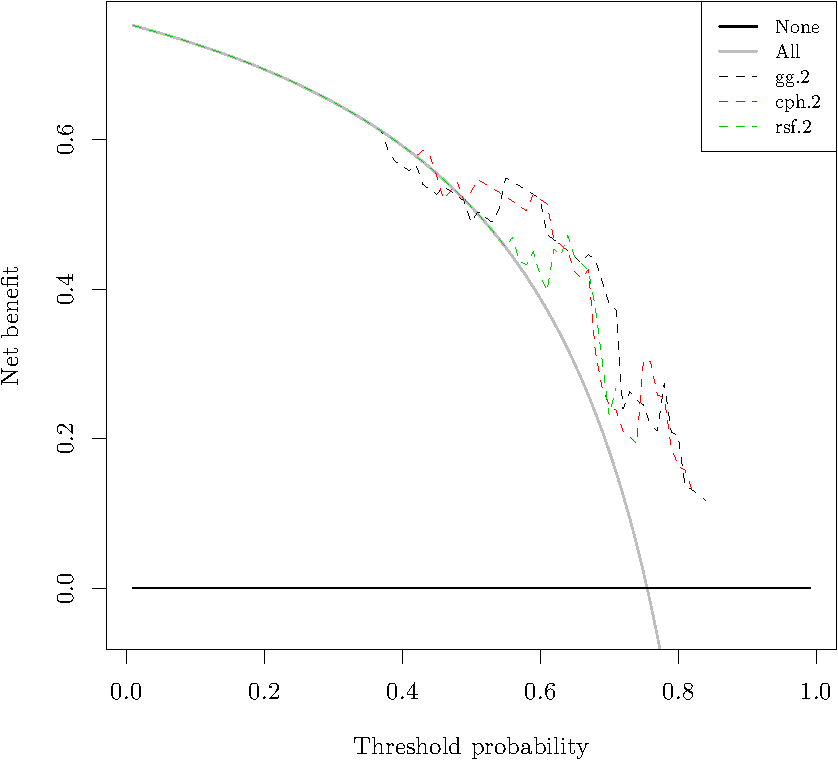
\includegraphics[width=\maxwidth]{figure/05-model-selection-dca-2} 

}


\begin{kframe}\begin{verbatim}
## $N
## [1] 198
## 
## $predictors
##      predictor harm.applied probability
## 1         gg.2            0        TRUE
## 2        cph.2            0        TRUE
## 3        rsf.2            0        TRUE
## 4  mskcc.pre.2            0        TRUE
## 5 mskcc.post.2            0        TRUE
## 
## $interventions.avoided.per
## [1] 100
## 
## $net.benefit
##    threshold        all none      gg.2      cph.2     rsf.2 mskcc.pre.2
## 1       0.01   0.588071    0  0.588071  0.5880714  0.588071    0.588071
## 2       0.02   0.583868    0  0.583868  0.5838680  0.583868    0.583868
## 3       0.03   0.579578    0  0.579578  0.5795780  0.579578    0.579578
## 4       0.04   0.575199    0  0.575199  0.5751986  0.575199    0.575199
## 5       0.05   0.570727    0  0.570727  0.5707270  0.570727    0.570727
## 6       0.06   0.566160    0  0.566160  0.5661603  0.566160    0.566160
## 7       0.07   0.561495    0  0.561495  0.5614953  0.561495    0.561495
## 8       0.08   0.556729    0  0.556729  0.5567290  0.556729    0.556729
## 9       0.09   0.551858    0  0.551858  0.5518578  0.551858    0.551858
## 10      0.10   0.546878    0  0.546878  0.5468785  0.546878    0.546878
## 11      0.11   0.541787    0  0.541787  0.5417872  0.541787    0.541787
## 12      0.12   0.536580    0  0.536580  0.5365803  0.536580    0.536580
## 13      0.13   0.531254    0  0.531254  0.5312536  0.531254    0.531254
## 14      0.14   0.525803    0  0.525803  0.5258031  0.525803    0.525803
## 15      0.15   0.520224    0  0.520224  0.5202243  0.520224    0.520224
## 16      0.16   0.514513    0  0.514513  0.5145127  0.514513    0.514513
## 17      0.17   0.508663    0  0.508663  0.5086634  0.508663    0.508663
## 18      0.18   0.502672    0  0.502672  0.5026715  0.502672    0.502672
## 19      0.19   0.496532    0  0.496532  0.4965317  0.496532    0.496532
## 20      0.20   0.490238    0  0.490238  0.4902383  0.490238    0.490238
## 21      0.21   0.483786    0  0.483786  0.4837856  0.483786    0.483786
## 22      0.22   0.477167    0  0.477167  0.4771675  0.477167    0.477167
## 23      0.23   0.470377    0  0.470377  0.4703775  0.470377    0.470377
## 24      0.24   0.463409    0  0.463409  0.4634087  0.463409    0.463409
## 25      0.25   0.456254    0  0.456254  0.4562542  0.456254    0.456254
## 26      0.26   0.448906    0  0.448906  0.4489063  0.448906    0.448906
## 27      0.27   0.441357    0  0.441357  0.4413570  0.441357    0.441357
## 28      0.28   0.433598    0  0.433598  0.4335981  0.433598    0.433598
## 29      0.29   0.425621    0  0.425621  0.4256206  0.425621    0.425621
## 30      0.30   0.417415    0  0.417415  0.4174152  0.417415    0.417415
## 31      0.31   0.408972    0  0.408972  0.4089719  0.408972    0.408972
## 32      0.32   0.400280    0  0.400280  0.4002804  0.400280    0.400280
## 33      0.33   0.391329    0  0.394265  0.3913293  0.391329    0.391329
## 34      0.34   0.382107    0  0.385164  0.3821070  0.382107    0.382107
## 35      0.35   0.372601    0  0.375783  0.3726010  0.372601    0.372601
## 36      0.36   0.362798    0  0.366108  0.3627979  0.362798    0.362798
## 37      0.37   0.352684    0  0.356127  0.3526836  0.352684    0.359576
## 38      0.38   0.342243    0  0.345823  0.3422430  0.342243    0.358381
## 39      0.39   0.331460    0  0.335182  0.3314601  0.331460    0.352422
## 40      0.40   0.320318    0  0.324186  0.3203177  0.320318    0.346536
## 41      0.41   0.308798    0  0.316842  0.3087977  0.308798    0.340628
## 42      0.42   0.296880    0  0.305237  0.2968804  0.296880    0.323984
## 43      0.43   0.284545    0  0.306295  0.2845450  0.284545    0.261932
## 44      0.44   0.271769    0  0.292657  0.2717690  0.271769    0.106312
## 45      0.45   0.258528    0  0.280623  0.2632071  0.258528    0.030762
## 46      0.46   0.244797    0  0.268143  0.2496563  0.244797   -0.003554
## 47      0.47   0.230548    0  0.248463  0.2298125  0.230548   -0.003907
## 48      0.48   0.215751    0  0.235564  0.2169548  0.215751   -0.004274
## 49      0.49   0.200374    0  0.216786  0.2020961  0.200374   -0.004654
## 50      0.50   0.184381    0  0.199590  0.1979246  0.184381   -0.005051
## 51      0.51   0.167736    0  0.191570  0.1822772  0.167736   -0.005463
## 52      0.52   0.150397    0  0.189628  0.1914811  0.150397   -0.005892
## 53      0.53   0.132321    0  0.158620  0.2075295  0.132321   -0.006340
## 54      0.54   0.113458    0  0.172338  0.2092613  0.120040   -0.006807
## 55      0.55   0.093757    0  0.165249  0.2016539  0.107446   -0.007295
## 56      0.56   0.073161    0  0.165299  0.1865321  0.081457   -0.007805
## 57      0.57   0.051606    0  0.175484  0.1834252  0.067168   -0.013390
## 58      0.58   0.029025    0  0.161504  0.1687929  0.109337   -0.013949
## 59      0.59   0.005343    0  0.149410  0.1506160  0.113494   -0.014536
## 60      0.60  -0.019523    0  0.146603  0.1519405  0.111146   -0.015152
## 61      0.61  -0.045665    0  0.132102  0.1219518  0.121122   -0.015799
## 62      0.62  -0.073183    0  0.111276  0.1049051  0.099386   -0.016481
## 63      0.63  -0.102187    0  0.104899  0.0878113  0.086335   -0.017199
## 64      0.64  -0.132804    0  0.097075  0.0797604  0.067576   -0.017957
## 65      0.65  -0.165170    0  0.085143  0.1024069  0.070268    0.005051
## 66      0.66  -0.199439    0  0.067742  0.0731230  0.046247    0.005051
## 67      0.67  -0.235786    0  0.010112  0.0495696  0.026681    0.005051
## 68      0.68  -0.274404    0  0.014298  0.0667518  0.024238    0.005051
## 69      0.69  -0.315514    0  0.008267  0.0570675  0.022454    0.005051
## 70      0.70  -0.359365    0  0.010728  0.0183144 -0.002186    0.005051
## 71      0.71  -0.406239    0  0.023764  0.0323611 -0.026743    0.005051
## 72      0.72  -0.456462    0 -0.005057  0.0149382 -0.019112    0.005051
## 73      0.73  -0.510405    0  0.069085  0.0081694  0.050416    0.005051
## 74      0.74  -0.568498    0  0.054648  0.0009491  0.028083    0.005051
## 75      0.75  -0.631237    0  0.039056  0.0109565  0.031769    0.005051
## 76      0.76  -0.699206    0  0.010737 -0.0060533  0.042494    0.005051
## 77      0.77  -0.773084    0 -0.029448 -0.0238759  0.043494    0.005051
## 78      0.78  -0.853679    0 -0.029554 -0.0485375  0.031926    0.005051
## 79      0.79  -0.941949    0 -0.018673 -0.0688796  0.019257          NA
## 80      0.80  -1.039047    0 -0.037433 -0.0374332  0.005321          NA
## 81      0.81  -1.146365    0 -0.041161 -0.0585421 -0.010082          NA
## 82      0.82  -1.265608    0 -0.060394 -0.0902927 -0.032548          NA
## 83      0.83  -1.398879    0 -0.088730 -0.0887304 -0.036450          NA
## 84      0.84  -1.548808    0 -0.086287 -0.0862866 -0.056090          NA
## 85      0.85  -1.718729    0 -0.057720 -0.1132512 -0.094688          NA
## 86      0.86  -1.912924    0 -0.083488 -0.1496243 -0.123256          NA
## 87      0.87  -2.136995    0 -0.135557 -0.1852209 -0.180579          NA
## 88      0.88  -2.398411    0 -0.130648 -0.2230930 -0.117845          NA
## 89      0.89  -2.707358    0 -0.090160 -0.2713815        NA          NA
## 90      0.90  -3.078094    0 -0.105246 -0.2873377        NA          NA
## 91      0.91  -3.531215    0 -0.160244 -0.3157645        NA          NA
## 92      0.92  -4.097617    0 -0.212121 -0.4073387        NA          NA
## 93      0.93  -4.825848    0 -0.179936 -0.4156983        NA          NA
## 94      0.94  -5.796823    0 -0.247475 -0.2696153        NA          NA
## 95      0.95  -7.156187    0 -0.324296 -0.3063973        NA          NA
## 96      0.96  -9.195234    0 -0.181818 -0.1824495        NA          NA
## 97      0.97 -12.593645    0 -0.117845 -0.1230487        NA          NA
## 98      0.98 -19.390468    0        NA         NA        NA          NA
## 99      0.99 -39.780936    0        NA         NA        NA          NA
##    mskcc.post.2
## 1      0.588071
## 2      0.583868
## 3      0.579578
## 4      0.575199
## 5      0.570727
## 6      0.566160
## 7      0.561495
## 8      0.556729
## 9      0.551858
## 10     0.546878
## 11     0.541787
## 12     0.536580
## 13     0.531254
## 14     0.525803
## 15     0.520224
## 16     0.514513
## 17     0.508663
## 18     0.502672
## 19     0.496532
## 20     0.490238
## 21     0.483786
## 22     0.477167
## 23     0.470377
## 24     0.463409
## 25     0.456254
## 26     0.451087
## 27     0.443637
## 28     0.438366
## 29     0.435596
## 30     0.435683
## 31     0.425530
## 32     0.407691
## 33     0.396793
## 34     0.389643
## 35     0.377965
## 36     0.375035
## 37     0.367111
## 38     0.351077
## 39     0.331653
## 40     0.309274
## 41     0.289669
## 42     0.261943
## 43     0.249775
## 44     0.256111
## 45     0.210665
## 46     0.182000
## 47     0.188886
## 48     0.150492
## 49     0.135305
## 50     0.104494
## 51     0.096397
## 52     0.078417
## 53     0.061267
## 54     0.037378
## 55     0.002300
## 56     0.007896
## 57     0.002349
## 58    -0.005400
## 59    -0.007133
## 60     0.002841
## 61     0.009065
## 62     0.002481
## 63           NA
## 64           NA
## 65           NA
## 66           NA
## 67           NA
## 68           NA
## 69           NA
## 70           NA
## 71           NA
## 72           NA
## 73           NA
## 74           NA
## 75           NA
## 76           NA
## 77           NA
## 78           NA
## 79           NA
## 80           NA
## 81           NA
## 82           NA
## 83           NA
## 84           NA
## 85           NA
## 86           NA
## 87           NA
## 88           NA
## 89           NA
## 90           NA
## 91           NA
## 92           NA
## 93           NA
## 94           NA
## 95           NA
## 96           NA
## 97           NA
## 98           NA
## 99           NA
## 
## $interventions.avoided
##    threshold    gg.2    cph.2   rsf.2 mskcc.pre.2 mskcc.post.2
## 1       0.01  0.0000  0.00000  0.0000      0.0000      0.00000
## 2       0.02  0.0000  0.00000  0.0000      0.0000      0.00000
## 3       0.03  0.0000  0.00000  0.0000      0.0000      0.00000
## 4       0.04  0.0000  0.00000  0.0000      0.0000      0.00000
## 5       0.05  0.0000  0.00000  0.0000      0.0000      0.00000
## 6       0.06  0.0000  0.00000  0.0000      0.0000      0.00000
## 7       0.07  0.0000  0.00000  0.0000      0.0000      0.00000
## 8       0.08  0.0000  0.00000  0.0000      0.0000      0.00000
## 9       0.09  0.0000  0.00000  0.0000      0.0000      0.00000
## 10      0.10  0.0000  0.00000  0.0000      0.0000      0.00000
## 11      0.11  0.0000  0.00000  0.0000      0.0000      0.00000
## 12      0.12  0.0000  0.00000  0.0000      0.0000      0.00000
## 13      0.13  0.0000  0.00000  0.0000      0.0000      0.00000
## 14      0.14  0.0000  0.00000  0.0000      0.0000      0.00000
## 15      0.15  0.0000  0.00000  0.0000      0.0000      0.00000
## 16      0.16  0.0000  0.00000  0.0000      0.0000      0.00000
## 17      0.17  0.0000  0.00000  0.0000      0.0000      0.00000
## 18      0.18  0.0000  0.00000  0.0000      0.0000      0.00000
## 19      0.19  0.0000  0.00000  0.0000      0.0000      0.00000
## 20      0.20  0.0000  0.00000  0.0000      0.0000      0.00000
## 21      0.21  0.0000  0.00000  0.0000      0.0000      0.00000
## 22      0.22  0.0000  0.00000  0.0000      0.0000      0.00000
## 23      0.23  0.0000  0.00000  0.0000      0.0000      0.00000
## 24      0.24  0.0000  0.00000  0.0000      0.0000      0.00000
## 25      0.25  0.0000  0.00000  0.0000      0.0000      0.00000
## 26      0.26  0.0000  0.00000  0.0000      0.0000      0.62065
## 27      0.27  0.0000  0.00000  0.0000      0.0000      0.61636
## 28      0.28  0.0000  0.00000  0.0000      0.0000      1.22606
## 29      0.29  0.0000  0.00000  0.0000      0.0000      2.44225
## 30      0.30  0.0000  0.00000  0.0000      0.0000      4.26248
## 31      0.31  0.0000  0.00000  0.0000      0.0000      3.68553
## 32      0.32  0.0000  0.00000  0.0000      0.0000      1.57477
## 33      0.33  0.5961  0.00000  0.0000      0.0000      1.10936
## 34      0.34  0.5934  0.00000  0.0000      0.0000      1.46295
## 35      0.35  0.5909  0.00000  0.0000      0.0000      0.99618
## 36      0.36  0.5885  0.00000  0.0000      0.0000      2.17543
## 37      0.37  0.5863  0.00000  0.0000      1.1735      2.45650
## 38      0.38  0.5841  0.00000  0.0000      2.6330      1.44129
## 39      0.39  0.5821  0.00000  0.0000      3.2787      0.03024
## 40      0.40  0.5802  0.00000  0.0000      3.9327     -1.65649
## 41      0.41  1.1576  0.00000  0.0000      4.5804     -2.75266
## 42      0.42  1.1541  0.00000  0.0000      3.7429     -4.82473
## 43      0.43  2.8832  0.00000  0.0000     -2.9976     -4.60908
## 44      0.44  2.6585  0.00000  0.0000    -21.0582     -1.99279
## 45      0.45  2.7004  0.57184  0.0000    -27.8381     -5.84997
## 46      0.46  2.7405  0.57039  0.0000    -29.1543     -7.37192
## 47      0.47  2.0201 -0.08298  0.0000    -26.4386     -4.69812
## 48      0.48  2.1464  0.13038  0.0000    -23.8360     -7.06973
## 49      0.49  1.7082  0.17926  0.0000    -21.3397     -6.77248
## 50      0.50  1.5208  1.35433  0.0000    -18.9432     -7.98875
## 51      0.51  2.2899  1.39710  0.0000    -16.6407     -6.85411
## 52      0.52  3.6213  3.79236  0.0000    -14.4267     -6.64428
## 53      0.53  2.3323  6.66947  0.0000    -12.2963     -6.30094
## 54      0.54  5.0157  8.16103  0.5607    -10.2448     -6.48092
## 55      0.55  5.8494  8.82793  1.1200     -8.2679     -7.48287
## 56      0.56  7.2395  8.90776  0.6518     -6.3616     -5.12797
## 57      0.57  9.3451  9.94424  1.1739     -4.9032     -3.71588
## 58      0.58  9.5933 10.12110  5.8157     -3.1119     -2.49289
## 59      0.59 10.0114 10.09524  7.5156     -1.3814     -0.86701
## 60      0.60 11.0751 11.43092  8.7113      0.2915      1.49095
## 61      0.61 11.3654 10.71649 10.6634      1.9095      3.49913
## 62      0.62 11.3055 10.91505 10.5768      3.4753      4.63744
## 63      0.63 12.1622 11.15866 11.0719      4.9914           NA
## 64      0.64 12.9307 11.95673 11.2714      6.4601           NA
## 65      0.65 13.4783 14.40797 12.6774      9.1657           NA
## 66      0.66 13.7639 14.04109 12.6566     10.5343           NA
## 67      0.67 12.1114 14.05482 12.9275     11.8621           NA
## 68      0.68 13.5860 16.05440 14.0538     13.1508           NA
## 69      0.69 14.5467 16.73917 15.1841     14.4022           NA
## 70      0.70 15.8611 16.18624 15.3076     15.6178           NA
## 71      0.71 17.5635 17.91466 15.5006     16.7992           NA
## 72      0.72 17.5546 18.33223 17.0081     17.9477           NA
## 73      0.73 21.4332 19.18015 20.7427     19.0648           NA
## 74      0.74 21.8943 20.00758 20.9609     20.1517           NA
## 75      0.75 22.3431 21.40646 22.1002     21.2096           NA
## 76      0.76 22.4192 21.88902 23.4221     22.2397           NA
## 77      0.77 22.2125 22.37895 24.3913     23.2430           NA
## 78      0.78 23.2445 22.70912 24.9786     24.2206           NA
## 79      0.79 24.5428 23.20818 25.5511          NA           NA
## 80      0.80 25.0403 25.04034 26.1092          NA           NA
## 81      0.81 25.9245 25.51683 26.6536          NA           NA
## 82      0.82 26.4559 25.79959 27.0672          NA           NA
## 83      0.83 26.8344 26.83436 27.9052          NA           NA
## 84      0.84 27.8576 27.85756 28.4327          NA           NA
## 85      0.85 29.3119 28.33196 28.6595          NA           NA
## 86      0.86 29.7815 28.70488 29.1341          NA           NA
## 87      0.87 29.9065 29.16444 29.2338          NA           NA
## 88      0.88 30.9241 29.66343 31.0986          NA           NA
## 89      0.89 32.3474 30.10757      NA          NA           NA
## 90      0.90 33.0316 31.00840      NA          NA           NA
## 91      0.91 33.3393 31.80116      NA          NA           NA
## 92      0.92 33.7869 32.08938      NA          NA           NA
## 93      0.93 34.9692 33.19467      NA          NA           NA
## 94      0.94 35.4214 35.28005      NA          NA           NA
## 95      0.95 35.9573 36.05153      NA          NA           NA
## 96      0.96 37.5559 37.55327      NA          NA           NA
## 97      0.97 38.5849 38.56886      NA          NA           NA
## 98      0.98      NA       NA      NA          NA           NA
## 99      0.99      NA       NA      NA          NA           NA
\end{verbatim}
\begin{alltt}
\hlkwd{stdca}\hlstd{(}\hlkwc{data} \hlstd{= temp.data,} \hlkwc{outcome} \hlstd{=} \hlstr{"DSD"}\hlstd{,} \hlkwc{ttoutcome} \hlstd{=} \hlstr{"Time"}\hlstd{,} \hlkwc{predictors} \hlstd{=} \hlkwd{c}\hlstd{(}\hlstr{"gg.3"}\hlstd{,} \hlstr{"cph.3"}\hlstd{,} \hlstr{"rsf.3"}\hlstd{,} \hlstr{"mskcc.pre.3"}\hlstd{,} \hlstr{"mskcc.post.3"}\hlstd{),} \hlkwc{timepoint} \hlstd{=} \hlnum{365}\hlopt{*}\hlnum{3}\hlstd{,} \hlkwc{probability} \hlstd{=} \hlkwd{rep}\hlstd{(}\hlnum{TRUE}\hlstd{,} \hlnum{5}\hlstd{))}
\end{alltt}
\begin{verbatim}
## [1] "rsf.3: No observations with risk greater than 95% that have followup through the timepoint selected, and therefore net benefit not calculable in this range."       
## [2] "mskcc.pre.3: No observations with risk greater than 91%, and therefore net benefit not calculable in this range."                                                   
## [3] "mskcc.post.3: No observations with risk greater than 78% that have followup through the timepoint selected, and therefore net benefit not calculable in this range."
\end{verbatim}
\end{kframe}

{\centering 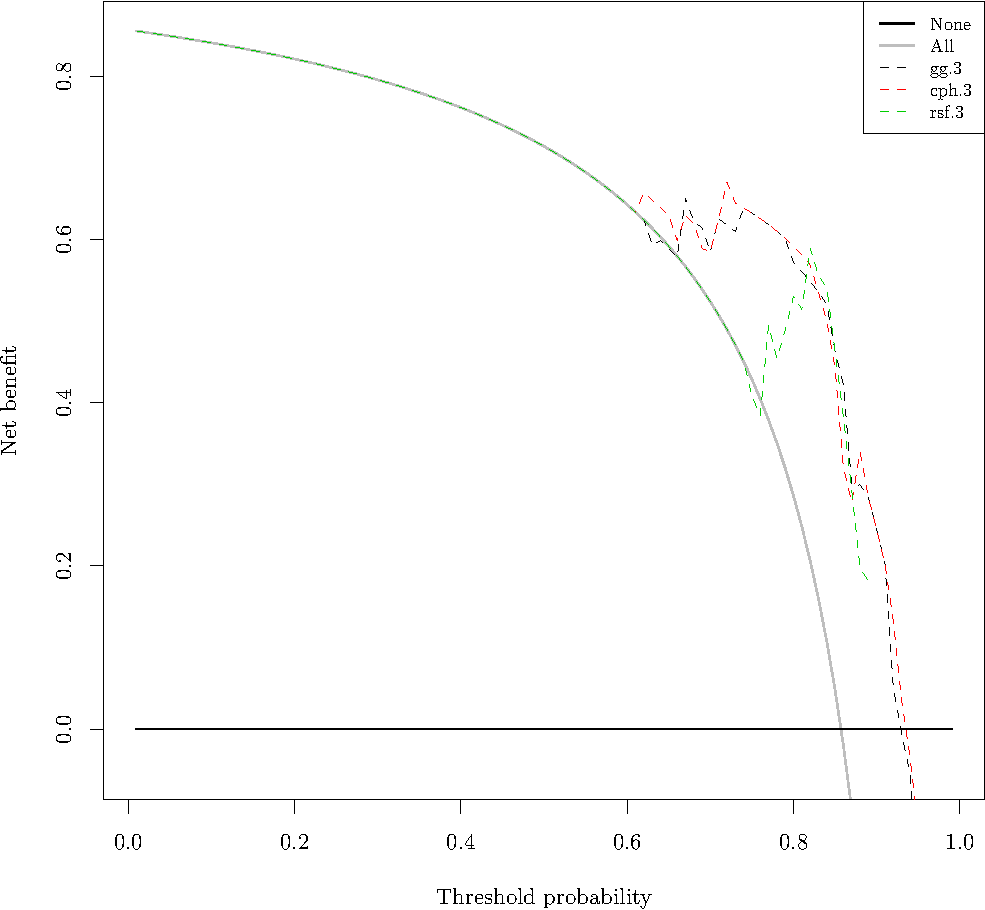
\includegraphics[width=\maxwidth]{figure/05-model-selection-dca-3} 

}


\begin{kframe}\begin{verbatim}
## $N
## [1] 198
## 
## $predictors
##      predictor harm.applied probability
## 1         gg.3            0        TRUE
## 2        cph.3            0        TRUE
## 3        rsf.3            0        TRUE
## 4  mskcc.pre.3            0        TRUE
## 5 mskcc.post.3            0        TRUE
## 
## $interventions.avoided.per
## [1] 100
## 
## $net.benefit
##    threshold       all none     gg.3     cph.3     rsf.3 mskcc.pre.3
## 1       0.01   0.78021    0  0.78021  0.780211  0.780211    0.780211
## 2       0.02   0.77797    0  0.77797  0.777968  0.777968    0.777968
## 3       0.03   0.77568    0  0.77568  0.775679  0.775679    0.775679
## 4       0.04   0.77334    0  0.77334  0.773342  0.773342    0.773342
## 5       0.05   0.77096    0  0.77096  0.770956  0.770956    0.770956
## 6       0.06   0.76852    0  0.76852  0.768520  0.768520    0.768520
## 7       0.07   0.76603    0  0.76603  0.766031  0.766031    0.766031
## 8       0.08   0.76349    0  0.76349  0.763488  0.763488    0.763488
## 9       0.09   0.76089    0  0.76089  0.760889  0.760889    0.760889
## 10      0.10   0.75823    0  0.75823  0.758232  0.758232    0.758232
## 11      0.11   0.75552    0  0.75552  0.755515  0.755515    0.755515
## 12      0.12   0.75274    0  0.75274  0.752737  0.752737    0.752737
## 13      0.13   0.74989    0  0.74989  0.749895  0.749895    0.749895
## 14      0.14   0.74699    0  0.74699  0.746987  0.746987    0.746987
## 15      0.15   0.74401    0  0.74401  0.744010  0.744010    0.744010
## 16      0.16   0.74096    0  0.74096  0.740963  0.740963    0.740963
## 17      0.17   0.73784    0  0.73784  0.737842  0.737842    0.737842
## 18      0.18   0.73464    0  0.73464  0.734645  0.734645    0.734645
## 19      0.19   0.73137    0  0.73137  0.731369  0.731369    0.731369
## 20      0.20   0.72801    0  0.72801  0.728011  0.728011    0.728011
## 21      0.21   0.72457    0  0.72457  0.724568  0.724568    0.724568
## 22      0.22   0.72104    0  0.72104  0.721037  0.721037    0.721037
## 23      0.23   0.71741    0  0.71741  0.717414  0.717414    0.717414
## 24      0.24   0.71370    0  0.71370  0.713695  0.713695    0.713695
## 25      0.25   0.70988    0  0.70988  0.709878  0.709878    0.709878
## 26      0.26   0.70596    0  0.70596  0.705958  0.705958    0.705958
## 27      0.27   0.70193    0  0.70193  0.701930  0.701930    0.701930
## 28      0.28   0.69779    0  0.69779  0.697790  0.697790    0.697790
## 29      0.29   0.69353    0  0.69353  0.693533  0.693533    0.693533
## 30      0.30   0.68916    0  0.68916  0.689155  0.689155    0.689155
## 31      0.31   0.68465    0  0.68465  0.684650  0.684650    0.684650
## 32      0.32   0.68001    0  0.68001  0.680013  0.680013    0.680013
## 33      0.33   0.67524    0  0.67524  0.675237  0.675237    0.675237
## 34      0.34   0.67032    0  0.67032  0.670316  0.670316    0.670316
## 35      0.35   0.66524    0  0.66524  0.665244  0.665244    0.665244
## 36      0.36   0.66001    0  0.66001  0.660013  0.660013    0.660013
## 37      0.37   0.65462    0  0.65462  0.654617  0.654617    0.654617
## 38      0.38   0.64905    0  0.64905  0.649046  0.649046    0.649046
## 39      0.39   0.64329    0  0.64329  0.643293  0.643293    0.643293
## 40      0.40   0.63735    0  0.63735  0.637348  0.637348    0.637348
## 41      0.41   0.63120    0  0.63120  0.631201  0.631201    0.631201
## 42      0.42   0.62484    0  0.62484  0.624842  0.624842    0.624842
## 43      0.43   0.61826    0  0.61826  0.618261  0.618261    0.618261
## 44      0.44   0.61144    0  0.61144  0.611444  0.611444    0.611444
## 45      0.45   0.60438    0  0.60438  0.604379  0.604379    0.604379
## 46      0.46   0.59705    0  0.59705  0.597053  0.597053    0.597053
## 47      0.47   0.58945    0  0.58945  0.589450  0.589450    0.589450
## 48      0.48   0.58155    0  0.58155  0.581555  0.581555    0.581555
## 49      0.49   0.57335    0  0.57335  0.573350  0.573350    0.573350
## 50      0.50   0.56482    0  0.56482  0.564817  0.564817    0.564817
## 51      0.51   0.55594    0  0.55594  0.555936  0.555936    0.552251
## 52      0.52   0.54668    0  0.54668  0.546685  0.546685    0.545592
## 53      0.53   0.53704    0  0.53704  0.537040  0.537040    0.523438
## 54      0.54   0.52698    0  0.52698  0.526975  0.526975    0.521261
## 55      0.55   0.51646    0  0.52357  0.516463  0.516463    0.519226
## 56      0.56   0.50547    0  0.51285  0.505474  0.505474    0.509906
## 57      0.57   0.49397    0  0.50164  0.493973  0.493973    0.450034
## 58      0.58   0.48193    0  0.48990  0.481925  0.481925    0.328353
## 59      0.59   0.46929    0  0.47758  0.469289  0.469289    0.059611
## 60      0.60   0.45602    0  0.46464  0.456021  0.456021   -0.005051
## 61      0.61   0.44207    0  0.45105  0.442073  0.442073   -0.010749
## 62      0.62   0.42739    0  0.43673  0.427391  0.427391   -0.011430
## 63      0.63   0.41192    0  0.42165  0.410991  0.411915   -0.012149
## 64      0.64   0.39558    0  0.40572  0.395059  0.395579   -0.012907
## 65      0.65   0.37831    0  0.38348  0.388865  0.378310   -0.013709
## 66      0.66   0.36003    0  0.36564  0.360888  0.360025   -0.014557
## 67      0.67   0.34063    0  0.34672  0.342592  0.340632   -0.015458
## 68      0.68   0.32003    0  0.32506  0.365005  0.320027   -0.016414
## 69      0.69   0.29809    0  0.30599  0.359166  0.298092   -0.017432
## 70      0.70   0.27470    0  0.27418  0.353291  0.274695   -0.018519
## 71      0.71   0.24968    0  0.25222  0.345110  0.249685   -0.019680
## 72      0.72   0.22289    0  0.28222  0.319955  0.222888   -0.020924
## 73      0.73   0.19411    0  0.27617  0.292384  0.205558   -0.027310
## 74      0.74   0.16311    0  0.26996  0.275377  0.207393   -0.028749
## 75      0.75   0.12963    0  0.24835  0.253058  0.193470   -0.030303
## 76      0.76   0.09337    0  0.23931  0.228880  0.191085   -0.031987
## 77      0.77   0.05395    0  0.21590  0.213238  0.242216   -0.033816
## 78      0.78   0.01095    0  0.18189  0.185477  0.191137   -0.035813
## 79      0.79  -0.03615    0  0.15520  0.140073  0.137037   -0.037999
## 80      0.80  -0.08796    0  0.12499  0.153385  0.135222    0.005051
## 81      0.81  -0.14522    0  0.08723  0.112516  0.060068    0.005051
## 82      0.82  -0.20884    0  0.04583  0.080047  0.008168    0.005051
## 83      0.83  -0.27995    0  0.04404  0.109761 -0.021500    0.005051
## 84      0.84  -0.35995    0  0.03971  0.063845  0.006594    0.005051
## 85      0.85  -0.45061    0  0.07195  0.092500  0.065285    0.005051
## 86      0.86  -0.55422    0  0.08482  0.086003  0.108750    0.005051
## 87      0.87  -0.67378    0  0.07549  0.064280  0.153323    0.005051
## 88      0.88  -0.81326    0  0.02418 -0.004204  0.159205    0.005051
## 89      0.89  -0.97810    0 -0.03420 -0.074473  0.132422    0.005051
## 90      0.90  -1.17591    0 -0.09098 -0.056582  0.106061    0.005051
## 91      0.91  -1.41768    0 -0.01565 -0.027184  0.120611          NA
## 92      0.92  -1.71989    0 -0.01695 -0.022529  0.144231          NA
## 93      0.93  -2.10845    0 -0.02506 -0.090834  0.093764          NA
## 94      0.94  -2.62652    0 -0.02027 -0.008936  0.016835          NA
## 95      0.95  -3.35183    0 -0.04467 -0.005393        NA          NA
## 96      0.96  -4.43979    0 -0.05556 -0.086287        NA          NA
## 97      0.97  -6.25305    0 -0.01331 -0.226750        NA          NA
## 98      0.98  -9.87957    0 -0.11111 -0.256410        NA          NA
## 99      0.99 -20.75914    0 -0.40909 -0.350168        NA          NA
##    mskcc.post.3
## 1      0.780211
## 2      0.777968
## 3      0.775679
## 4      0.773342
## 5      0.770956
## 6      0.768520
## 7      0.766031
## 8      0.763488
## 9      0.760889
## 10     0.758232
## 11     0.755515
## 12     0.752737
## 13     0.749895
## 14     0.746987
## 15     0.744010
## 16     0.740963
## 17     0.737842
## 18     0.734645
## 19     0.731369
## 20     0.728011
## 21     0.724568
## 22     0.721037
## 23     0.717414
## 24     0.713695
## 25     0.709878
## 26     0.705958
## 27     0.701930
## 28     0.697790
## 29     0.693533
## 30     0.689155
## 31     0.684650
## 32     0.680013
## 33     0.675237
## 34     0.670316
## 35     0.665244
## 36     0.660013
## 37     0.658248
## 38     0.652817
## 39     0.651133
## 40     0.649571
## 41     0.651851
## 42     0.655117
## 43     0.648430
## 44     0.627034
## 45     0.590163
## 46     0.575938
## 47     0.570415
## 48     0.561708
## 49     0.561741
## 50     0.550016
## 51     0.534803
## 52     0.519843
## 53     0.478884
## 54     0.454252
## 55     0.442167
## 56     0.413379
## 57     0.374308
## 58     0.343137
## 59     0.330506
## 60     0.280300
## 61     0.274222
## 62     0.228301
## 63     0.151937
## 64     0.158286
## 65     0.141877
## 66     0.121667
## 67     0.098262
## 68     0.074435
## 69     0.050033
## 70     0.007552
## 71     0.006941
## 72    -0.002202
## 73    -0.017770
## 74    -0.026171
## 75    -0.011111
## 76    -0.020202
## 77    -0.009076
## 78           NA
## 79           NA
## 80           NA
## 81           NA
## 82           NA
## 83           NA
## 84           NA
## 85           NA
## 86           NA
## 87           NA
## 88           NA
## 89           NA
## 90           NA
## 91           NA
## 92           NA
## 93           NA
## 94           NA
## 95           NA
## 96           NA
## 97           NA
## 98           NA
## 99           NA
## 
## $interventions.avoided
##    threshold     gg.3    cph.3   rsf.3 mskcc.pre.3 mskcc.post.3
## 1       0.01  0.00000  0.00000  0.0000     0.00000       0.0000
## 2       0.02  0.00000  0.00000  0.0000     0.00000       0.0000
## 3       0.03  0.00000  0.00000  0.0000     0.00000       0.0000
## 4       0.04  0.00000  0.00000  0.0000     0.00000       0.0000
## 5       0.05  0.00000  0.00000  0.0000     0.00000       0.0000
## 6       0.06  0.00000  0.00000  0.0000     0.00000       0.0000
## 7       0.07  0.00000  0.00000  0.0000     0.00000       0.0000
## 8       0.08  0.00000  0.00000  0.0000     0.00000       0.0000
## 9       0.09  0.00000  0.00000  0.0000     0.00000       0.0000
## 10      0.10  0.00000  0.00000  0.0000     0.00000       0.0000
## 11      0.11  0.00000  0.00000  0.0000     0.00000       0.0000
## 12      0.12  0.00000  0.00000  0.0000     0.00000       0.0000
## 13      0.13  0.00000  0.00000  0.0000     0.00000       0.0000
## 14      0.14  0.00000  0.00000  0.0000     0.00000       0.0000
## 15      0.15  0.00000  0.00000  0.0000     0.00000       0.0000
## 16      0.16  0.00000  0.00000  0.0000     0.00000       0.0000
## 17      0.17  0.00000  0.00000  0.0000     0.00000       0.0000
## 18      0.18  0.00000  0.00000  0.0000     0.00000       0.0000
## 19      0.19  0.00000  0.00000  0.0000     0.00000       0.0000
## 20      0.20  0.00000  0.00000  0.0000     0.00000       0.0000
## 21      0.21  0.00000  0.00000  0.0000     0.00000       0.0000
## 22      0.22  0.00000  0.00000  0.0000     0.00000       0.0000
## 23      0.23  0.00000  0.00000  0.0000     0.00000       0.0000
## 24      0.24  0.00000  0.00000  0.0000     0.00000       0.0000
## 25      0.25  0.00000  0.00000  0.0000     0.00000       0.0000
## 26      0.26  0.00000  0.00000  0.0000     0.00000       0.0000
## 27      0.27  0.00000  0.00000  0.0000     0.00000       0.0000
## 28      0.28  0.00000  0.00000  0.0000     0.00000       0.0000
## 29      0.29  0.00000  0.00000  0.0000     0.00000       0.0000
## 30      0.30  0.00000  0.00000  0.0000     0.00000       0.0000
## 31      0.31  0.00000  0.00000  0.0000     0.00000       0.0000
## 32      0.32  0.00000  0.00000  0.0000     0.00000       0.0000
## 33      0.33  0.00000  0.00000  0.0000     0.00000       0.0000
## 34      0.34  0.00000  0.00000  0.0000     0.00000       0.0000
## 35      0.35  0.00000  0.00000  0.0000     0.00000       0.0000
## 36      0.36  0.00000  0.00000  0.0000     0.00000       0.0000
## 37      0.37  0.00000  0.00000  0.0000     0.00000       0.6183
## 38      0.38  0.00000  0.00000  0.0000     0.00000       0.6153
## 39      0.39  0.00000  0.00000  0.0000     0.00000       1.2264
## 40      0.40  0.00000  0.00000  0.0000     0.00000       1.8335
## 41      0.41  0.00000  0.00000  0.0000     0.00000       2.9716
## 42      0.42  0.00000  0.00000  0.0000     0.00000       4.1808
## 43      0.43  0.00000  0.00000  0.0000     0.00000       3.9993
## 44      0.44  0.00000  0.00000  0.0000     0.00000       1.9842
## 45      0.45  0.00000  0.00000  0.0000     0.00000      -1.7375
## 46      0.46  0.00000  0.00000  0.0000     0.00000      -2.4787
## 47      0.47  0.00000  0.00000  0.0000     0.00000      -2.1466
## 48      0.48  0.00000  0.00000  0.0000     0.00000      -2.1501
## 49      0.49  0.00000  0.00000  0.0000     0.00000      -1.2083
## 50      0.50  0.00000  0.00000  0.0000     0.00000      -1.4801
## 51      0.51  0.00000  0.00000  0.0000    -0.35408      -2.0304
## 52      0.52  0.00000  0.00000  0.0000    -0.10088      -2.4777
## 53      0.53  0.00000  0.00000  0.0000    -1.20618      -5.1572
## 54      0.54  0.00000  0.00000  0.0000    -0.48675      -6.1950
## 55      0.55  0.58124  0.00000  0.0000     0.22599      -6.0788
## 56      0.56  0.57988  0.00000  0.0000     0.34822      -7.2360
## 57      0.57  0.57856  0.00000  0.0000    -3.31476      -9.0274
## 58      0.58  0.57730  0.00000  0.0000   -11.12074     -10.0502
## 59      0.59  0.57607  0.00000  0.0000   -28.46915      -9.6442
## 60      0.60  0.57489  0.00000  0.0000   -30.73813     -11.7148
## 61      0.61  0.57374  0.00000  0.0000   -28.95090     -10.7315
## 62      0.62  0.57264  0.00000  0.0000   -26.89548     -12.2023
## 63      0.63  0.57156 -0.05426  0.0000   -24.90532     -15.2686
## 64      0.64  0.57052 -0.02928  0.0000   -22.97735     -13.3477
## 65      0.65  0.27824  0.56831  0.0000   -21.10870     -12.7310
## 66      0.66  0.28933  0.04444  0.0000   -19.29668     -12.2790
## 67      0.67  0.30008  0.09654  0.0000   -17.53874     -11.9376
## 68      0.68  0.23692  2.11662  0.0000   -15.83251     -11.5573
## 69      0.69  0.35482  2.74388  0.0000   -14.17574     -11.1447
## 70      0.70 -0.02191  3.36841  0.0000   -12.56630     -11.4490
## 71      0.71  0.10356  3.89763  0.0000   -11.00220      -9.9149
## 72      0.72  2.30740  3.77482  0.0000    -9.48155      -8.7535
## 73      0.73  3.03529  3.63493  0.4236    -8.18936      -7.8365
## 74      0.74  3.75409  3.94451  1.5559    -6.74099      -6.6504
## 75      0.75  3.95736  4.11414  2.1279    -5.33124      -4.6915
## 76      0.76  4.60876  4.27930  3.0858    -3.95860      -3.5865
## 77      0.77  4.83750  4.75793  5.6235    -2.62160      -1.8826
## 78      0.78  4.82157  4.92261  5.0823    -1.31889           NA
## 79      0.79  5.08658  4.68439  4.6037    -0.04916           NA
## 80      0.80  5.32357  6.03356  5.5795     2.32519           NA
## 81      0.81  5.45241  6.04562  4.8154     3.52482           NA
## 82      0.82  5.59026  6.34144  4.7636     4.69519           NA
## 83      0.83  6.63586  7.98203  5.2936     5.83735           NA
## 84      0.84  7.61259  8.07222  6.9817     6.95232           NA
## 85      0.85  9.22164  9.58428  9.1040     8.04106           NA
## 86      0.86 10.40304 10.42232 10.7926     9.10448           NA
## 87      0.87 11.19596 11.02848 12.3590    10.14345           NA
## 88      0.88 11.41969 11.03261 13.2609    11.15881           NA
## 89      0.89 11.66625 11.16847 13.7256    12.15135           NA
## 90      0.90 12.05486 12.43702 14.2442    13.12183           NA
## 91      0.91 13.86627 13.75218 15.2139          NA           NA
## 92      0.92 14.80820 14.75969 16.2098          NA           NA
## 93      0.93 15.68139 15.18635 16.5758          NA           NA
## 94      0.94 16.63565 16.70801 16.8725          NA           NA
## 95      0.95 17.40608 17.61282      NA          NA           NA
## 96      0.96 18.26763 18.13958      NA          NA           NA
## 97      0.97 19.29817 18.63803      NA          NA           NA
## 98      0.98 19.93563 19.63910      NA          NA           NA
## 99      0.99 20.55561 20.61513      NA          NA           NA
\end{verbatim}
\end{kframe}
\end{knitrout}


\subsection{Brier score}
\begin{knitrout}
\definecolor{shadecolor}{rgb}{0.969, 0.969, 0.969}\color{fgcolor}\begin{kframe}
\begin{alltt}
\hlstd{calcIBS} \hlkwb{=} \hlkwa{function}\hlstd{(}\hlkwc{surv}\hlstd{,} \hlkwc{pred}\hlstd{,} \hlkwc{pred_times}\hlstd{,} \hlkwc{max_time}\hlstd{)}
\hlstd{\{}
        \hlkwd{stopifnot}\hlstd{(}\hlkwd{nrow}\hlstd{(surv)} \hlopt{==} \hlkwd{nrow}\hlstd{(pred)} \hlopt{&&} \hlkwd{length}\hlstd{(pred_times)} \hlopt{==} \hlkwd{ncol}\hlstd{(pred))}

        \hlstd{n} \hlkwb{=} \hlkwd{nrow}\hlstd{(surv)}
        \hlstd{marg_survfit} \hlkwb{=} \hlkwd{survfit}\hlstd{(surv} \hlopt{~} \hlnum{1}\hlstd{)}
        \hlstd{marg_censfit} \hlkwb{=} \hlkwd{survfit}\hlstd{(}\hlkwd{Surv}\hlstd{(surv[,}\hlnum{1}\hlstd{],} \hlopt{!}\hlstd{surv[,}\hlnum{2}\hlstd{])} \hlopt{~} \hlnum{1}\hlstd{)}
        \hlstd{marg_surv_func} \hlkwb{=} \hlkwd{approxfun}\hlstd{(marg_survfit}\hlopt{$}\hlstd{time, marg_survfit}\hlopt{$}\hlstd{surv,} \hlkwc{method} \hlstd{=} \hlstr{"constant"}\hlstd{,} \hlkwc{yleft} \hlstd{=} \hlnum{1}\hlstd{,} \hlkwc{yright} \hlstd{=} \hlnum{0}\hlstd{,} \hlkwc{rule} \hlstd{=} \hlnum{2}\hlopt{:}\hlnum{1}\hlstd{,} \hlkwc{f} \hlstd{=} \hlnum{0}\hlstd{)}
        \hlstd{marg_cens_func} \hlkwb{=} \hlkwd{approxfun}\hlstd{(marg_censfit}\hlopt{$}\hlstd{time, marg_censfit}\hlopt{$}\hlstd{surv,} \hlkwc{method} \hlstd{=} \hlstr{"constant"}\hlstd{,} \hlkwc{yleft} \hlstd{=} \hlnum{1}\hlstd{,} \hlkwc{yright} \hlstd{=} \hlnum{0}\hlstd{,} \hlkwc{rule} \hlstd{=} \hlnum{2}\hlopt{:}\hlnum{1}\hlstd{,} \hlkwc{f} \hlstd{=} \hlnum{0}\hlstd{)}

        \hlstd{pred_funcs} \hlkwb{=} \hlkwd{apply}\hlstd{(pred,} \hlnum{1}\hlstd{,} \hlkwa{function}\hlstd{(}\hlkwc{pat_preds}\hlstd{)} \hlkwd{approxfun}\hlstd{(pred_times, pat_preds,} \hlkwc{yleft} \hlstd{=} \hlnum{1}\hlstd{,} \hlkwc{yright} \hlstd{=} \hlkwd{min}\hlstd{(pat_preds),} \hlkwc{rule} \hlstd{=} \hlnum{2}\hlstd{))}

        \hlstd{indiv_patient_bsc} \hlkwb{=} \hlkwa{function}\hlstd{(}\hlkwc{pat_i}\hlstd{,} \hlkwc{tstars}\hlstd{)}
        \hlstd{\{}
                \hlstd{observed_time} \hlkwb{=} \hlstd{surv[pat_i,} \hlnum{1}\hlstd{]}
                \hlstd{observed_event} \hlkwb{=} \hlstd{surv[pat_i,} \hlnum{2}\hlstd{]}
                \hlstd{pred_func} \hlkwb{=} \hlstd{pred_funcs[[pat_i]]}
                \hlstd{category} \hlkwb{=} \hlnum{1}\hlopt{*}\hlstd{(observed_time} \hlopt{<=} \hlstd{tstars} \hlopt{&} \hlstd{observed_event)} \hlopt{+} \hlnum{2}\hlopt{*}\hlstd{(observed_time} \hlopt{>} \hlstd{tstars)} \hlopt{+} \hlnum{3}\hlopt{*}\hlstd{(observed_time} \hlopt{<=} \hlstd{tstars} \hlopt{& !}\hlstd{observed_event)}
                \hlstd{bsc} \hlkwb{=} \hlkwd{rep}\hlstd{(}\hlnum{NA}\hlstd{,} \hlkwd{length}\hlstd{(tstars))}
                \hlstd{bsc[category} \hlopt{==} \hlnum{1}\hlstd{]} \hlkwb{=} \hlkwd{pred_func}\hlstd{(tstars[category} \hlopt{==} \hlnum{1}\hlstd{])}\hlopt{^}\hlnum{2} \hlopt{/} \hlkwd{marg_cens_func}\hlstd{(observed_time)}
                \hlstd{bsc[category} \hlopt{==} \hlnum{2}\hlstd{]} \hlkwb{=} \hlstd{(}\hlnum{1} \hlopt{-} \hlkwd{pred_func}\hlstd{(tstars[category} \hlopt{==} \hlnum{2}\hlstd{]))}\hlopt{^}\hlnum{2} \hlopt{/} \hlkwd{marg_cens_func}\hlstd{(tstars[category} \hlopt{==} \hlnum{2}\hlstd{])}
                \hlstd{bsc[category} \hlopt{==} \hlnum{3}\hlstd{]} \hlkwb{=} \hlnum{0}
                \hlstd{bsc}
        \hlstd{\}}

        \hlstd{bsc_func} \hlkwb{=} \hlkwa{function}\hlstd{(}\hlkwc{tstars}\hlstd{) \{} \hlkwd{rowMeans}\hlstd{(}\hlkwd{sapply}\hlstd{(}\hlnum{1}\hlopt{:}\hlstd{n,} \hlkwa{function}\hlstd{(}\hlkwc{pat_i}\hlstd{)} \hlkwd{indiv_patient_bsc}\hlstd{(pat_i, tstars))) \}}

        \hlstd{weight_func} \hlkwb{=} \hlkwa{function}\hlstd{(}\hlkwc{tstars}\hlstd{) \{ (}\hlnum{1} \hlopt{-} \hlkwd{marg_surv_func}\hlstd{(tstars))} \hlopt{/} \hlstd{(}\hlnum{1} \hlopt{-} \hlkwd{marg_surv_func}\hlstd{(max_time)) \}}

        \hlcom{# Be slack and do trapezoidal int. with a fine grid.  It should be possible }
        \hlcom{# to calulate the int. exactly but I cbfed.}
        \hlstd{int_grid} \hlkwb{=} \hlkwd{seq}\hlstd{(}\hlnum{0}\hlstd{, max_time,} \hlkwc{length.out} \hlstd{=} \hlnum{1e3}\hlstd{)}
        \hlstd{bsc_vals} \hlkwb{=} \hlkwd{bsc_func}\hlstd{(int_grid)}
        \hlstd{weight_vals} \hlkwb{=} \hlkwd{weight_func}\hlstd{(int_grid)}
        \hlstd{int_vals} \hlkwb{=} \hlstd{bsc_vals} \hlopt{*} \hlstd{weight_vals}
        \hlstd{ibsc} \hlkwb{=} \hlstd{(}\hlnum{2}\hlopt{*}\hlkwd{sum}\hlstd{(int_vals)} \hlopt{-} \hlstd{int_vals[}\hlnum{1}\hlstd{]} \hlopt{-} \hlstd{int_vals[}\hlkwd{length}\hlstd{(int_vals)])} \hlopt{*} \hlstd{(}\hlkwd{diff}\hlstd{(}\hlkwd{range}\hlstd{(int_grid)))} \hlopt{/} \hlstd{(}\hlnum{2}\hlopt{*}\hlkwd{length}\hlstd{(int_vals))}

        \hlkwd{return}\hlstd{(}\hlkwd{list}\hlstd{(}\hlkwc{bsc} \hlstd{= bsc_vals,} \hlkwc{weights} \hlstd{= weight_vals,} \hlkwc{eval_times} \hlstd{= int_grid,} \hlkwc{ibsc} \hlstd{= ibsc))}
\hlstd{\}}

\hlstd{calcBSsingle} \hlkwb{=} \hlkwa{function}\hlstd{(}\hlkwc{surv}\hlstd{,} \hlkwc{pred}\hlstd{,} \hlkwc{pred_time}\hlstd{)}
\hlstd{\{}
        \hlstd{n} \hlkwb{=} \hlkwd{nrow}\hlstd{(surv)}
        \hlstd{obs_time} \hlkwb{=} \hlstd{surv[,}\hlnum{1}\hlstd{]}
        \hlstd{obs_event} \hlkwb{=} \hlstd{surv[,}\hlnum{2}\hlstd{]}
        \hlstd{marg_censfit} \hlkwb{=} \hlkwd{survfit}\hlstd{(}\hlkwd{Surv}\hlstd{(obs_time,} \hlopt{!}\hlstd{obs_event)} \hlopt{~} \hlnum{1}\hlstd{)}
        \hlstd{marg_cens_func} \hlkwb{=} \hlkwd{approxfun}\hlstd{(marg_censfit}\hlopt{$}\hlstd{time, marg_censfit}\hlopt{$}\hlstd{surv,} \hlkwc{method} \hlstd{=} \hlstr{"constant"}\hlstd{,} \hlkwc{yleft} \hlstd{=} \hlnum{1}\hlstd{,} \hlkwc{yright} \hlstd{=} \hlnum{0}\hlstd{,} \hlkwc{rule} \hlstd{=} \hlnum{2}\hlopt{:}\hlnum{1}\hlstd{,} \hlkwc{f} \hlstd{=} \hlnum{0}\hlstd{)}

        \hlstd{brier_val} \hlkwb{=} \hlkwd{rep}\hlstd{(}\hlnum{NA}\hlstd{, n)}
        \hlstd{cat} \hlkwb{=} \hlnum{1}\hlopt{*}\hlkwd{I}\hlstd{(obs_time} \hlopt{<=} \hlstd{pred_time} \hlopt{&} \hlstd{obs_event)} \hlopt{+} \hlnum{2}\hlopt{*}\hlkwd{I}\hlstd{(obs_time} \hlopt{>} \hlstd{pred_time)} \hlopt{+} \hlnum{3}\hlopt{*}\hlkwd{I}\hlstd{(obs_time} \hlopt{<=} \hlstd{pred_time} \hlopt{& !}\hlstd{obs_event)}
        \hlstd{brier_val[cat} \hlopt{==} \hlnum{1}\hlstd{]} \hlkwb{=} \hlstd{(pred[cat} \hlopt{==} \hlnum{1}\hlstd{])}\hlopt{^}\hlnum{2} \hlopt{/} \hlkwd{marg_cens_func}\hlstd{(obs_time[cat} \hlopt{==} \hlnum{1}\hlstd{])}
        \hlstd{brier_val[cat} \hlopt{==} \hlnum{2}\hlstd{]} \hlkwb{=} \hlstd{(}\hlnum{1}\hlopt{-}\hlstd{pred[cat} \hlopt{==} \hlnum{2}\hlstd{])}\hlopt{^}\hlnum{2} \hlopt{/} \hlkwd{marg_cens_func}\hlstd{(pred_time)}
        \hlstd{brier_val[cat} \hlopt{==} \hlnum{3}\hlstd{]} \hlkwb{=} \hlnum{0}

        \hlkwd{mean}\hlstd{(brier_val)}
\hlstd{\}}
\end{alltt}
\end{kframe}
\end{knitrout}


\begin{knitrout}
\definecolor{shadecolor}{rgb}{0.969, 0.969, 0.969}\color{fgcolor}\begin{kframe}
\begin{alltt}
\hlstd{mskcc_post.12mo.glasgow.brier} \hlkwb{=} \hlkwd{calcBSsingle}\hlstd{(}\hlkwd{Surv}\hlstd{(data.glasgow}\hlopt{$}\hlstd{Time, data.glasgow}\hlopt{$}\hlstd{DSD), mskcc_post.12mo.glasgow,} \hlnum{12}\hlopt{/}\hlnum{12}\hlopt{*}\hlnum{365.25}\hlstd{)}
\hlstd{mskcc_post.24mo.glasgow.brier} \hlkwb{=} \hlkwd{calcBSsingle}\hlstd{(}\hlkwd{Surv}\hlstd{(data.glasgow}\hlopt{$}\hlstd{Time, data.glasgow}\hlopt{$}\hlstd{DSD), mskcc_post.24mo.glasgow,} \hlnum{24}\hlopt{/}\hlnum{12}\hlopt{*}\hlnum{365.25}\hlstd{)}
\hlstd{mskcc_post.36mo.glasgow.brier} \hlkwb{=} \hlkwd{calcBSsingle}\hlstd{(}\hlkwd{Surv}\hlstd{(data.glasgow}\hlopt{$}\hlstd{Time, data.glasgow}\hlopt{$}\hlstd{DSD), mskcc_post.36mo.glasgow,} \hlnum{36}\hlopt{/}\hlnum{12}\hlopt{*}\hlnum{365.25}\hlstd{)}
\hlstd{mskcc_pre.12mo.glasgow.brier} \hlkwb{=} \hlkwd{calcBSsingle}\hlstd{(}\hlkwd{Surv}\hlstd{(data.glasgow}\hlopt{$}\hlstd{Time, data.glasgow}\hlopt{$}\hlstd{DSD), mskcc_pre.12mo.glasgow,} \hlnum{12}\hlopt{/}\hlnum{12}\hlopt{*}\hlnum{365.25}\hlstd{)}
\hlstd{mskcc_pre.24mo.glasgow.brier} \hlkwb{=} \hlkwd{calcBSsingle}\hlstd{(}\hlkwd{Surv}\hlstd{(data.glasgow}\hlopt{$}\hlstd{Time, data.glasgow}\hlopt{$}\hlstd{DSD), mskcc_pre.24mo.glasgow,} \hlnum{24}\hlopt{/}\hlnum{12}\hlopt{*}\hlnum{365.25}\hlstd{)}
\hlstd{mskcc_pre.36mo.glasgow.brier} \hlkwb{=} \hlkwd{calcBSsingle}\hlstd{(}\hlkwd{Surv}\hlstd{(data.glasgow}\hlopt{$}\hlstd{Time, data.glasgow}\hlopt{$}\hlstd{DSD), mskcc_pre.36mo.glasgow,} \hlnum{36}\hlopt{/}\hlnum{12}\hlopt{*}\hlnum{365.25}\hlstd{)}
\hlstd{gg.path.glasgow.brier} \hlkwb{=} \hlkwd{calcIBS}\hlstd{(}\hlkwd{Surv}\hlstd{(data.glasgow}\hlopt{$}\hlstd{Time, data.glasgow}\hlopt{$}\hlstd{DSD),} \hlkwd{t}\hlstd{(}\hlkwd{sapply}\hlstd{(gg.path.glasgow,} \hlkwa{function}\hlstd{(}\hlkwc{x}\hlstd{) x[,}\hlnum{2}\hlstd{])), gg.path.glasgow[[}\hlnum{1}\hlstd{]][,}\hlnum{1}\hlstd{],} \hlnum{10}\hlopt{*}\hlnum{365.25}\hlstd{)}

\hlstd{km0.path.glasgow.brier} \hlkwb{=} \hlkwd{calcIBS}\hlstd{(}\hlkwd{Surv}\hlstd{(data.glasgow}\hlopt{$}\hlstd{Time, data.glasgow}\hlopt{$}\hlstd{DSD),} \hlkwd{matrix}\hlstd{(fit.km0}\hlopt{$}\hlstd{surv,} \hlkwc{nrow} \hlstd{=} \hlkwd{nrow}\hlstd{(data.glasgow),} \hlkwc{ncol} \hlstd{=} \hlkwd{length}\hlstd{(fit.km0}\hlopt{$}\hlstd{time),} \hlkwc{byrow} \hlstd{=} \hlnum{TRUE}\hlstd{), fit.km0}\hlopt{$}\hlstd{time,} \hlnum{10}\hlopt{*}\hlnum{365.25}\hlstd{)}

\hlstd{temp.cph.pred} \hlkwb{=} \hlkwd{survfit}\hlstd{(fit.cph,} \hlkwc{newdata} \hlstd{= data.glasgow)}
\hlstd{temp.cph.pred.expanded_strata} \hlkwb{=} \hlkwd{rep}\hlstd{(}\hlkwd{names}\hlstd{(temp.cph.pred}\hlopt{$}\hlstd{strata), temp.cph.pred}\hlopt{$}\hlstd{strata)}
\hlstd{temp.cph.pred_funcs} \hlkwb{=} \hlkwd{sapply}\hlstd{(}\hlkwd{rownames}\hlstd{(data.glasgow),} \hlkwa{function}\hlstd{(}\hlkwc{pat_id}\hlstd{) \{}
        \hlkwd{approxfun}\hlstd{(temp.cph.pred}\hlopt{$}\hlstd{time[temp.cph.pred.expanded_strata} \hlopt{==} \hlstd{pat_id], temp.cph.pred}\hlopt{$}\hlstd{surv[temp.cph.pred.expanded_strata} \hlopt{==} \hlstd{pat_id],} \hlkwc{method} \hlstd{=} \hlstr{"constant"}\hlstd{,} \hlkwc{f} \hlstd{=} \hlnum{0}\hlstd{,} \hlkwc{yleft} \hlstd{=} \hlnum{1}\hlstd{,} \hlkwc{rule} \hlstd{=} \hlnum{2}\hlstd{)}
\hlstd{\})}
\hlstd{cph.path.glasgow.brier} \hlkwb{=} \hlkwd{calcIBS}\hlstd{(}\hlkwd{Surv}\hlstd{(data.glasgow}\hlopt{$}\hlstd{Time, data.glasgow}\hlopt{$}\hlstd{DSD),}
        \hlkwd{t}\hlstd{(}\hlkwd{sapply}\hlstd{(temp.cph.pred_funcs[}\hlkwd{rownames}\hlstd{(data.glasgow)],} \hlkwa{function}\hlstd{(}\hlkwc{f}\hlstd{)} \hlkwd{f}\hlstd{(}\hlkwd{c}\hlstd{(}\hlnum{12}\hlstd{,} \hlnum{24}\hlstd{,} \hlnum{36}\hlstd{)}\hlopt{/}\hlnum{12}\hlopt{*}\hlnum{365.25}\hlstd{))),} \hlkwd{c}\hlstd{(}\hlnum{12}\hlstd{,} \hlnum{24}\hlstd{,} \hlnum{36}\hlstd{)}\hlopt{/}\hlnum{12}\hlopt{*}\hlnum{365.25}\hlstd{,} \hlnum{10}\hlopt{*}\hlnum{365.25}\hlstd{)}

\hlstd{gg2.path.glasgow.brier} \hlkwb{=} \hlkwd{calcIBS}\hlstd{(}\hlkwd{Surv}\hlstd{(data.glasgow}\hlopt{$}\hlstd{Time, data.glasgow}\hlopt{$}\hlstd{DSD),} \hlkwd{t}\hlstd{(}\hlkwd{sapply}\hlstd{(gg2.path.glasgow,} \hlkwa{function}\hlstd{(}\hlkwc{x}\hlstd{) x[,}\hlnum{2}\hlstd{])), gg2.path.glasgow[[}\hlnum{1}\hlstd{]][,}\hlnum{1}\hlstd{],} \hlnum{10}\hlopt{*}\hlnum{365.25}\hlstd{)}

\hlstd{temp.rsf.pred} \hlkwb{=} \hlkwd{predict}\hlstd{(fit.rsf,} \hlkwc{newdata} \hlstd{= data.glasgow)}
\hlstd{rsf.path.glasgow.brier} \hlkwb{=} \hlkwd{calcIBS}\hlstd{(}\hlkwd{Surv}\hlstd{(data.glasgow}\hlopt{$}\hlstd{Time, data.glasgow}\hlopt{$}\hlstd{DSD),} \hlkwd{t}\hlstd{(}\hlkwd{apply}\hlstd{(temp.rsf.pred}\hlopt{$}\hlstd{survival,} \hlnum{1}\hlstd{,} \hlkwa{function}\hlstd{(}\hlkwc{patpreds}\hlstd{)} \hlkwd{approx}\hlstd{(temp.rsf.pred}\hlopt{$}\hlstd{time.interest, patpreds,} \hlkwd{c}\hlstd{(}\hlnum{12}\hlstd{,} \hlnum{24}\hlstd{,} \hlnum{36}\hlstd{)}\hlopt{/}\hlnum{12}\hlopt{*}\hlnum{365.25}\hlstd{)}\hlopt{$}\hlstd{y)),} \hlkwd{c}\hlstd{(}\hlnum{12}\hlstd{,} \hlnum{24}\hlstd{,} \hlnum{36}\hlstd{)}\hlopt{/}\hlnum{12}\hlopt{*}\hlnum{365.25}\hlstd{,} \hlnum{10}\hlopt{*}\hlnum{365.25}\hlstd{)}

\hlkwd{plot}\hlstd{(gg.path.glasgow.brier}\hlopt{$}\hlstd{bsc} \hlopt{~} \hlstd{gg.path.glasgow.brier}\hlopt{$}\hlstd{eval_times,} \hlkwc{col} \hlstd{=} \hlstr{"aquamarine"}\hlstd{,} \hlkwc{type} \hlstd{=} \hlstr{"l"}\hlstd{,} \hlkwc{ylim} \hlstd{=} \hlkwd{c}\hlstd{(}\hlnum{0}\hlstd{,} \hlnum{0.3}\hlstd{),} \hlkwc{xlab} \hlstd{=} \hlstr{"Time from diagnosis"}\hlstd{,} \hlkwc{ylab} \hlstd{=} \hlstr{"Brier score"}\hlstd{)}
\hlkwd{lines}\hlstd{(km0.path.glasgow.brier}\hlopt{$}\hlstd{bsc} \hlopt{~} \hlstd{km0.path.glasgow.brier}\hlopt{$}\hlstd{eval_times,} \hlkwc{col} \hlstd{=} \hlstr{"grey"}\hlstd{)}
\hlkwd{lines}\hlstd{(cph.path.glasgow.brier}\hlopt{$}\hlstd{bsc} \hlopt{~} \hlstd{cph.path.glasgow.brier}\hlopt{$}\hlstd{eval_times,} \hlkwc{col} \hlstd{=} \hlstr{"pink"}\hlstd{)}
\hlkwd{lines}\hlstd{(gg2.path.glasgow.brier}\hlopt{$}\hlstd{bsc} \hlopt{~} \hlstd{gg2.path.glasgow.brier}\hlopt{$}\hlstd{eval_times,} \hlkwc{col} \hlstd{=} \hlstr{"purple"}\hlstd{)}
\hlkwd{lines}\hlstd{(rsf.path.glasgow.brier}\hlopt{$}\hlstd{bsc} \hlopt{~} \hlstd{rsf.path.glasgow.brier}\hlopt{$}\hlstd{eval_times,} \hlkwc{col} \hlstd{=} \hlstr{"green"}\hlstd{)}
\hlkwd{points}\hlstd{(}\hlkwd{c}\hlstd{(}\hlnum{12}\hlstd{,} \hlnum{24}\hlstd{,} \hlnum{36}\hlstd{)}\hlopt{/}\hlnum{12}\hlopt{*}\hlnum{365.25}\hlstd{,} \hlkwd{c}\hlstd{(mskcc_post.12mo.glasgow.brier, mskcc_post.24mo.glasgow.brier, mskcc_post.36mo.glasgow.brier),} \hlkwc{col} \hlstd{=} \hlstr{"red"}\hlstd{,} \hlkwc{cex} \hlstd{=} \hlnum{1}\hlstd{)}
\hlkwd{points}\hlstd{(}\hlkwd{c}\hlstd{(}\hlnum{12}\hlstd{,} \hlnum{24}\hlstd{,} \hlnum{36}\hlstd{)}\hlopt{/}\hlnum{12}\hlopt{*}\hlnum{365.25}\hlstd{,} \hlkwd{c}\hlstd{(mskcc_pre.12mo.glasgow.brier, mskcc_pre.24mo.glasgow.brier, mskcc_pre.36mo.glasgow.brier),} \hlkwc{col} \hlstd{=} \hlstr{"blue"}\hlstd{,} \hlkwc{cex} \hlstd{=} \hlnum{1}\hlstd{)}
\hlkwd{abline}\hlstd{(}\hlkwc{h} \hlstd{=} \hlnum{0.25}\hlstd{,} \hlkwc{col} \hlstd{=} \hlstr{"grey"}\hlstd{,} \hlkwc{lty} \hlstd{=} \hlstr{"dotted"}\hlstd{)}
\hlkwd{legend}\hlstd{(}\hlstr{"topright"}\hlstd{,}
        \hlkwc{legend} \hlstd{=} \hlkwd{c}\hlstd{(}     \hlstr{"GG1 Preop"}\hlstd{,}    \hlstr{"GG2 Preop"}\hlstd{,}    \hlstr{"CP1 Preop"}\hlstd{,}    \hlstr{"RSF Preop"}\hlstd{,}    \hlstr{"KM0"}\hlstd{,}          \hlstr{"MSKCC Postop"}\hlstd{,}         \hlstr{"MSKCC Preop"}\hlstd{),}
        \hlkwc{pch} \hlstd{=} \hlkwd{c}\hlstd{(}        \hlnum{NA}\hlstd{,}                     \hlnum{NA}\hlstd{,}                     \hlnum{NA}\hlstd{,}                     \hlnum{NA}\hlstd{,}                     \hlnum{NA}\hlstd{,}             \hlnum{1}\hlstd{,}                                      \hlnum{1}\hlstd{),}
        \hlkwc{col} \hlstd{=} \hlkwd{c}\hlstd{(}        \hlstr{"aquamarine"}\hlstd{,}   \hlstr{"purple"}\hlstd{,}               \hlstr{"pink"}\hlstd{,}                 \hlstr{"green"}\hlstd{,}                \hlstr{"grey"}\hlstd{,}         \hlstr{"red"}\hlstd{,}                          \hlstr{"blue"}\hlstd{),}
        \hlkwc{lty} \hlstd{=} \hlkwd{c}\hlstd{(}        \hlstr{"solid"}\hlstd{,}                \hlstr{"solid"}\hlstd{,}                \hlstr{"solid"}\hlstd{,}                \hlstr{"solid"}\hlstd{,}                \hlstr{"solid"}\hlstd{,}        \hlnum{NA}\hlstd{,}                             \hlnum{NA}\hlstd{),}
        \hlkwc{inset} \hlstd{=} \hlnum{0.05}\hlstd{)}
\end{alltt}
\end{kframe}

{\centering 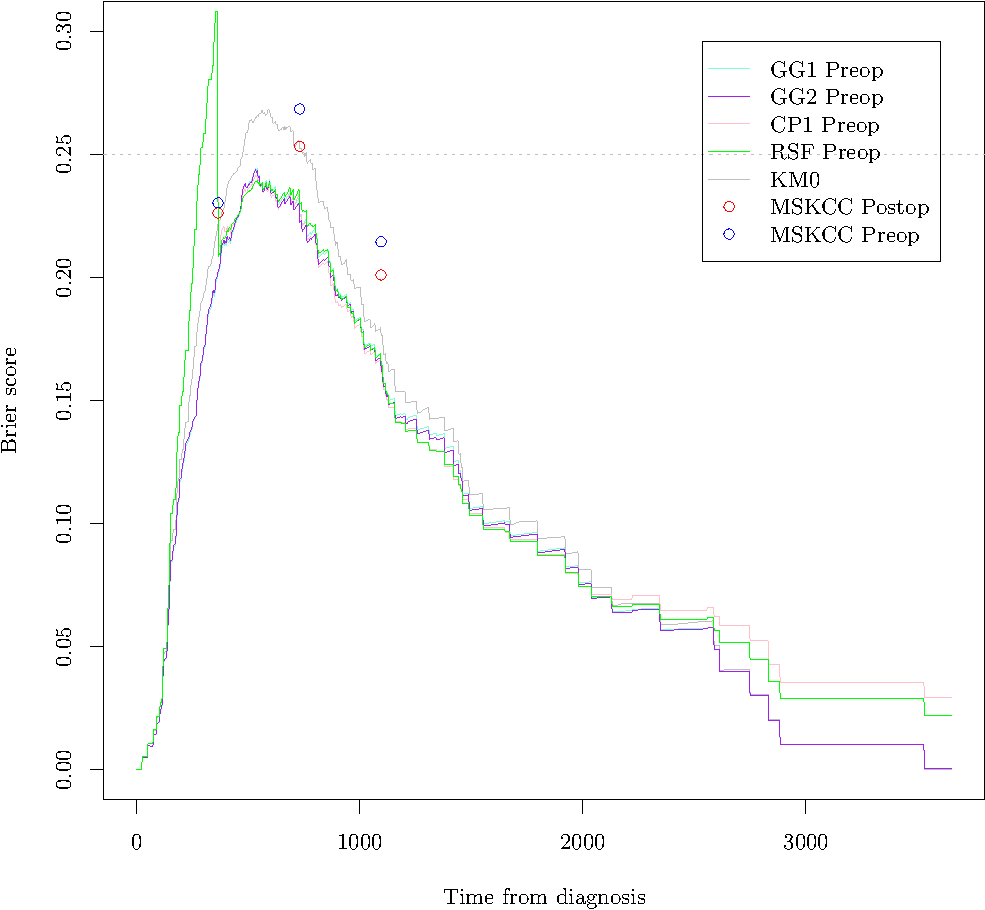
\includegraphics[width=\maxwidth]{figure/05-prob-bs-paths-1} 

}



\end{knitrout}


\begin{knitrout}
\definecolor{shadecolor}{rgb}{0.969, 0.969, 0.969}\color{fgcolor}\begin{kframe}
\begin{alltt}
\hlstd{probs_bs_boot_func} \hlkwb{=} \hlkwa{function}\hlstd{(}\hlkwc{d}\hlstd{,} \hlkwc{i}\hlstd{) \{}
        \hlstd{bs.mskcc.postop.12} \hlkwb{=} \hlkwd{calcBSsingle}\hlstd{(}\hlkwd{Surv}\hlstd{(d}\hlopt{$}\hlstd{Time[i], d}\hlopt{$}\hlstd{DSD[i]), mskcc_post.12mo.glasgow[i],} \hlnum{12}\hlopt{/}\hlnum{12}\hlopt{*}\hlnum{365.25}\hlstd{)}
        \hlstd{bs.mskcc.postop.24} \hlkwb{=} \hlkwd{calcBSsingle}\hlstd{(}\hlkwd{Surv}\hlstd{(d}\hlopt{$}\hlstd{Time[i], d}\hlopt{$}\hlstd{DSD[i]), mskcc_post.24mo.glasgow[i],} \hlnum{24}\hlopt{/}\hlnum{12}\hlopt{*}\hlnum{365.25}\hlstd{)}
        \hlstd{bs.mskcc.postop.36} \hlkwb{=} \hlkwd{calcBSsingle}\hlstd{(}\hlkwd{Surv}\hlstd{(d}\hlopt{$}\hlstd{Time[i], d}\hlopt{$}\hlstd{DSD[i]), mskcc_post.36mo.glasgow[i],} \hlnum{36}\hlopt{/}\hlnum{12}\hlopt{*}\hlnum{365.25}\hlstd{)}
        \hlstd{bs.mskcc.preop.12} \hlkwb{=} \hlkwd{calcBSsingle}\hlstd{(}\hlkwd{Surv}\hlstd{(d}\hlopt{$}\hlstd{Time[i], d}\hlopt{$}\hlstd{DSD[i]), mskcc_pre.12mo.glasgow[i],} \hlnum{12}\hlopt{/}\hlnum{12}\hlopt{*}\hlnum{365.25}\hlstd{)}
        \hlstd{bs.mskcc.preop.24} \hlkwb{=} \hlkwd{calcBSsingle}\hlstd{(}\hlkwd{Surv}\hlstd{(d}\hlopt{$}\hlstd{Time[i], d}\hlopt{$}\hlstd{DSD[i]), mskcc_pre.24mo.glasgow[i],} \hlnum{24}\hlopt{/}\hlnum{12}\hlopt{*}\hlnum{365.25}\hlstd{)}
        \hlstd{bs.mskcc.preop.36} \hlkwb{=} \hlkwd{calcBSsingle}\hlstd{(}\hlkwd{Surv}\hlstd{(d}\hlopt{$}\hlstd{Time[i], d}\hlopt{$}\hlstd{DSD[i]), mskcc_pre.36mo.glasgow[i],} \hlnum{36}\hlopt{/}\hlnum{12}\hlopt{*}\hlnum{365.25}\hlstd{)}

        \hlstd{bs.gg.vals} \hlkwb{=} \hlkwd{t}\hlstd{(}\hlkwd{sapply}\hlstd{(gg.path.glasgow[i],} \hlkwa{function}\hlstd{(}\hlkwc{path}\hlstd{)} \hlkwd{approx}\hlstd{(path[,}\hlnum{1}\hlstd{], path[,}\hlnum{2}\hlstd{],} \hlkwd{c}\hlstd{(}\hlnum{12}\hlstd{,} \hlnum{24}\hlstd{,} \hlnum{36}\hlstd{)}\hlopt{/}\hlnum{12}\hlopt{*}\hlnum{365.25}\hlstd{)}\hlopt{$}\hlstd{y))}
        \hlkwd{rownames}\hlstd{(bs.gg.vals)} \hlkwb{<-} \hlkwa{NULL}
        \hlstd{bs.gg.12} \hlkwb{=} \hlkwd{calcBSsingle}\hlstd{(}\hlkwd{Surv}\hlstd{(d}\hlopt{$}\hlstd{Time[i], d}\hlopt{$}\hlstd{DSD[i]), bs.gg.vals[,}\hlnum{1}\hlstd{],} \hlnum{12}\hlopt{/}\hlnum{12}\hlopt{*}\hlnum{365.25}\hlstd{)}
        \hlstd{bs.gg.24} \hlkwb{=} \hlkwd{calcBSsingle}\hlstd{(}\hlkwd{Surv}\hlstd{(d}\hlopt{$}\hlstd{Time[i], d}\hlopt{$}\hlstd{DSD[i]), bs.gg.vals[,}\hlnum{2}\hlstd{],} \hlnum{24}\hlopt{/}\hlnum{12}\hlopt{*}\hlnum{365.25}\hlstd{)}
        \hlstd{bs.gg.36} \hlkwb{=} \hlkwd{calcBSsingle}\hlstd{(}\hlkwd{Surv}\hlstd{(d}\hlopt{$}\hlstd{Time[i], d}\hlopt{$}\hlstd{DSD[i]), bs.gg.vals[,}\hlnum{3}\hlstd{],} \hlnum{36}\hlopt{/}\hlnum{12}\hlopt{*}\hlnum{365.25}\hlstd{)}

        \hlstd{cph.pred} \hlkwb{=} \hlkwd{survfit}\hlstd{(fit.cph,} \hlkwc{newdata} \hlstd{= d[i,])}
        \hlstd{cph.pred.expanded_strata} \hlkwb{=} \hlkwd{rep}\hlstd{(}\hlkwd{names}\hlstd{(cph.pred}\hlopt{$}\hlstd{strata), cph.pred}\hlopt{$}\hlstd{strata)}
        \hlstd{cph.pred_funcs} \hlkwb{=} \hlkwd{sapply}\hlstd{(}\hlkwd{rownames}\hlstd{(d)[i],} \hlkwa{function}\hlstd{(}\hlkwc{pat_id}\hlstd{) \{}
                \hlkwd{approxfun}\hlstd{(cph.pred}\hlopt{$}\hlstd{time[cph.pred.expanded_strata} \hlopt{==} \hlstd{pat_id], cph.pred}\hlopt{$}\hlstd{surv[cph.pred.expanded_strata} \hlopt{==} \hlstd{pat_id],} \hlkwc{method} \hlstd{=} \hlstr{"constant"}\hlstd{,} \hlkwc{f} \hlstd{=} \hlnum{0}\hlstd{,} \hlkwc{yleft} \hlstd{=} \hlnum{1}\hlstd{,} \hlkwc{rule} \hlstd{=} \hlnum{2}\hlstd{)}
        \hlstd{\})}
        \hlstd{bs.cph.12} \hlkwb{=} \hlkwd{calcBSsingle}\hlstd{(}\hlkwd{Surv}\hlstd{(d}\hlopt{$}\hlstd{Time[i], d}\hlopt{$}\hlstd{DSD[i]),} \hlkwd{sapply}\hlstd{(}\hlkwd{rownames}\hlstd{(d)[i],} \hlkwa{function}\hlstd{(}\hlkwc{pat_id}\hlstd{) cph.pred_funcs[[pat_id]](}\hlnum{12}\hlopt{/}\hlnum{12}\hlopt{*}\hlnum{365.25}\hlstd{)),} \hlnum{12}\hlopt{/}\hlnum{12}\hlopt{*}\hlnum{365.25}\hlstd{)}
        \hlstd{bs.cph.24} \hlkwb{=} \hlkwd{calcBSsingle}\hlstd{(}\hlkwd{Surv}\hlstd{(d}\hlopt{$}\hlstd{Time[i], d}\hlopt{$}\hlstd{DSD[i]),} \hlkwd{sapply}\hlstd{(}\hlkwd{rownames}\hlstd{(d)[i],} \hlkwa{function}\hlstd{(}\hlkwc{pat_id}\hlstd{) cph.pred_funcs[[pat_id]](}\hlnum{24}\hlopt{/}\hlnum{12}\hlopt{*}\hlnum{365.25}\hlstd{)),} \hlnum{24}\hlopt{/}\hlnum{12}\hlopt{*}\hlnum{365.25}\hlstd{)}
        \hlstd{bs.cph.36} \hlkwb{=} \hlkwd{calcBSsingle}\hlstd{(}\hlkwd{Surv}\hlstd{(d}\hlopt{$}\hlstd{Time[i], d}\hlopt{$}\hlstd{DSD[i]),} \hlkwd{sapply}\hlstd{(}\hlkwd{rownames}\hlstd{(d)[i],} \hlkwa{function}\hlstd{(}\hlkwc{pat_id}\hlstd{) cph.pred_funcs[[pat_id]](}\hlnum{36}\hlopt{/}\hlnum{12}\hlopt{*}\hlnum{365.25}\hlstd{)),} \hlnum{36}\hlopt{/}\hlnum{12}\hlopt{*}\hlnum{365.25}\hlstd{)}

        \hlstd{bs.km0.vals} \hlkwb{=} \hlkwd{approx}\hlstd{(fit.km0}\hlopt{$}\hlstd{time, fit.km0}\hlopt{$}\hlstd{surv,} \hlkwd{c}\hlstd{(}\hlnum{12}\hlstd{,} \hlnum{24}\hlstd{,} \hlnum{36}\hlstd{)}\hlopt{/}\hlnum{12}\hlopt{*}\hlnum{365.25}\hlstd{)}\hlopt{$}\hlstd{y}
        \hlstd{bs.km0.12} \hlkwb{=} \hlkwd{calcBSsingle}\hlstd{(}\hlkwd{Surv}\hlstd{(d}\hlopt{$}\hlstd{Time[i], d}\hlopt{$}\hlstd{DSD[i]),} \hlkwd{rep}\hlstd{(bs.km0.vals[}\hlnum{1}\hlstd{],} \hlkwd{nrow}\hlstd{(d[i,])),} \hlnum{12}\hlopt{/}\hlnum{12}\hlopt{*}\hlnum{365.25}\hlstd{)}
        \hlstd{bs.km0.24} \hlkwb{=} \hlkwd{calcBSsingle}\hlstd{(}\hlkwd{Surv}\hlstd{(d}\hlopt{$}\hlstd{Time[i], d}\hlopt{$}\hlstd{DSD[i]),} \hlkwd{rep}\hlstd{(bs.km0.vals[}\hlnum{2}\hlstd{],} \hlkwd{nrow}\hlstd{(d[i,])),} \hlnum{24}\hlopt{/}\hlnum{12}\hlopt{*}\hlnum{365.25}\hlstd{)}
        \hlstd{bs.km0.36} \hlkwb{=} \hlkwd{calcBSsingle}\hlstd{(}\hlkwd{Surv}\hlstd{(d}\hlopt{$}\hlstd{Time[i], d}\hlopt{$}\hlstd{DSD[i]),} \hlkwd{rep}\hlstd{(bs.km0.vals[}\hlnum{3}\hlstd{],} \hlkwd{nrow}\hlstd{(d[i,])),} \hlnum{36}\hlopt{/}\hlnum{12}\hlopt{*}\hlnum{365.25}\hlstd{)}

        \hlstd{result} \hlkwb{=} \hlkwd{c}\hlstd{(}
                \hlstd{bs.cph.12} \hlopt{-} \hlstd{bs.km0.12,                  bs.gg.12} \hlopt{-} \hlstd{bs.km0.12,                   bs.mskcc.postop.12} \hlopt{-} \hlstd{bs.km0.12,                 bs.mskcc.preop.12} \hlopt{-} \hlstd{bs.km0.12,}
                \hlstd{bs.cph.12} \hlopt{-} \hlstd{bs.mskcc.preop.12,  bs.gg.12} \hlopt{-} \hlstd{bs.mskcc.preop.12,   bs.mskcc.postop.12} \hlopt{-} \hlstd{bs.mskcc.preop.12,}
                \hlstd{bs.cph.12} \hlopt{-} \hlstd{bs.mskcc.postop.12, bs.gg.12} \hlopt{-} \hlstd{bs.mskcc.postop.12,}
                \hlstd{bs.cph.12} \hlopt{-} \hlstd{bs.gg.12,}
                \hlstd{bs.cph.24} \hlopt{-} \hlstd{bs.km0.24,                  bs.gg.24} \hlopt{-} \hlstd{bs.km0.24,                   bs.mskcc.postop.24} \hlopt{-} \hlstd{bs.km0.24,                 bs.mskcc.preop.24} \hlopt{-} \hlstd{bs.km0.24,}
                \hlstd{bs.cph.24} \hlopt{-} \hlstd{bs.mskcc.preop.24,  bs.gg.24} \hlopt{-} \hlstd{bs.mskcc.preop.24,   bs.mskcc.postop.24} \hlopt{-} \hlstd{bs.mskcc.preop.24,}
                \hlstd{bs.cph.24} \hlopt{-} \hlstd{bs.mskcc.postop.24, bs.gg.24} \hlopt{-} \hlstd{bs.mskcc.postop.24,}
                \hlstd{bs.cph.24} \hlopt{-} \hlstd{bs.gg.24,}
                \hlstd{bs.cph.36} \hlopt{-} \hlstd{bs.km0.36,                  bs.gg.36} \hlopt{-} \hlstd{bs.km0.36,                   bs.mskcc.postop.36} \hlopt{-} \hlstd{bs.km0.36,                 bs.mskcc.preop.36} \hlopt{-} \hlstd{bs.km0.36,}
                \hlstd{bs.cph.36} \hlopt{-} \hlstd{bs.mskcc.preop.36,  bs.gg.36} \hlopt{-} \hlstd{bs.mskcc.preop.36,   bs.mskcc.postop.36} \hlopt{-} \hlstd{bs.mskcc.preop.36,}
                \hlstd{bs.cph.36} \hlopt{-} \hlstd{bs.mskcc.postop.36, bs.gg.36} \hlopt{-} \hlstd{bs.mskcc.postop.36,}
                \hlstd{bs.cph.36} \hlopt{-} \hlstd{bs.gg.36)}
        \hlkwd{names}\hlstd{(result)} \hlkwb{<-} \hlkwa{NULL}
        \hlstd{result}
\hlstd{\}}

\hlkwd{set.seed}\hlstd{(}\hlnum{20150113}\hlstd{)}
\hlstd{deltaBrier.boot.glasgow} \hlkwb{=} \hlkwd{boot}\hlstd{(data.glasgow, probs_bs_boot_func,} \hlkwc{R} \hlstd{=} \hlnum{500}\hlstd{)}
\hlstd{deltaBrier.boot.glasgow.cis} \hlkwb{=} \hlkwd{t}\hlstd{(}\hlkwd{sapply}\hlstd{(}\hlnum{1}\hlopt{:}\hlkwd{ncol}\hlstd{(deltaBrier.boot.glasgow}\hlopt{$}\hlstd{t),} \hlkwa{function}\hlstd{(}\hlkwc{i}\hlstd{)} \hlkwd{boot.ci}\hlstd{(deltaBrier.boot.glasgow,} \hlkwc{index} \hlstd{= i,} \hlkwc{type} \hlstd{=} \hlstr{"bca"}\hlstd{)}\hlopt{$}\hlstd{bca))}
\hlkwd{colnames}\hlstd{(deltaBrier.boot.glasgow.cis)} \hlkwb{=} \hlkwd{c}\hlstd{(}\hlstr{"level"}\hlstd{,} \hlstr{"lowindex"}\hlstd{,} \hlstr{"highindex"}\hlstd{,} \hlstr{"lci"}\hlstd{,} \hlstr{"uci"}\hlstd{)}
\hlkwd{rownames}\hlstd{(deltaBrier.boot.glasgow.cis)} \hlkwb{=} \hlkwd{c}\hlstd{(}
        \hlstr{"12:cph-km0"}\hlstd{,} \hlstr{"12:gg-km0"}\hlstd{,} \hlstr{"12:post-km0"}\hlstd{,} \hlstr{"12:pre-km0"}\hlstd{,} \hlstr{"12:cph-pre"}\hlstd{,} \hlstr{"12:gg-pre"}\hlstd{,} \hlstr{"12:post-pre"}\hlstd{,} \hlstr{"12:cph-post"}\hlstd{,} \hlstr{"12:gg-post"}\hlstd{,} \hlstr{"12:cph-gg"}\hlstd{,}
        \hlstr{"24:cph-km0"}\hlstd{,} \hlstr{"24:gg-km0"}\hlstd{,} \hlstr{"24:post-km0"}\hlstd{,} \hlstr{"24:pre-km0"}\hlstd{,} \hlstr{"24:cph-pre"}\hlstd{,} \hlstr{"24:gg-pre"}\hlstd{,} \hlstr{"24:post-pre"}\hlstd{,} \hlstr{"24:cph-post"}\hlstd{,} \hlstr{"24:gg-post"}\hlstd{,} \hlstr{"24:cph-gg"}\hlstd{,}
        \hlstr{"36:cph-km0"}\hlstd{,} \hlstr{"36:gg-km0"}\hlstd{,} \hlstr{"36:post-km0"}\hlstd{,} \hlstr{"36:pre-km0"}\hlstd{,} \hlstr{"36:cph-pre"}\hlstd{,} \hlstr{"36:gg-pre"}\hlstd{,} \hlstr{"36:post-pre"}\hlstd{,} \hlstr{"36:cph-post"}\hlstd{,} \hlstr{"36:gg-post"}\hlstd{,} \hlstr{"36:cph-gg"}\hlstd{)}
\hlstd{deltaBrier.boot.glasgow}
\end{alltt}
\begin{verbatim}
## 
## ORDINARY NONPARAMETRIC BOOTSTRAP
## 
## 
## Call:
## boot(data = data.glasgow, statistic = probs_bs_boot_func, R = 500)
## 
## 
## Bootstrap Statistics :
##        original     bias    std. error
## t1*  -0.0107346 -1.403e-03    0.012699
## t2*  -0.0207374 -1.474e-03    0.012316
## t3*   0.0037324 -1.033e-03    0.014366
## t4*   0.0078972 -6.393e-04    0.014648
## t5*  -0.0186318 -7.634e-04    0.022123
## t6*  -0.0286346 -8.347e-04    0.021348
## t7*  -0.0041648 -3.935e-04    0.003150
## t8*  -0.0144669 -3.699e-04    0.021773
## t9*  -0.0244698 -4.413e-04    0.021043
## t10*  0.0100028  7.136e-05    0.002871
## t11* -0.0269945 -3.682e-04    0.010481
## t12* -0.0276310 -5.277e-04    0.011371
## t13*  0.0012760 -2.046e-03    0.020184
## t14*  0.0164211 -1.435e-03    0.020014
## t15* -0.0434155  1.067e-03    0.021542
## t16* -0.0440521  9.069e-04    0.021258
## t17* -0.0151451 -6.114e-04    0.005561
## t18* -0.0282704  1.678e-03    0.021498
## t19* -0.0289069  1.518e-03    0.021349
## t20*  0.0006365  1.596e-04    0.003258
## t21* -0.0148527 -5.323e-04    0.006927
## t22* -0.0125841 -4.967e-04    0.006582
## t23*  0.0250004 -2.048e-03    0.018127
## t24*  0.0384405 -1.355e-03    0.017079
## t25* -0.0532932  8.226e-04    0.016095
## t26* -0.0510246  8.582e-04    0.016575
## t27* -0.0134401 -6.928e-04    0.005662
## t28* -0.0398531  1.515e-03    0.016962
## t29* -0.0375845  1.551e-03    0.017465
## t30* -0.0022686 -3.562e-05    0.002097
\end{verbatim}
\begin{alltt}
\hlstd{deltaBrier.boot.glasgow.cis}
\end{alltt}
\begin{verbatim}
##             level lowindex highindex       lci        uci
## 12:cph-km0   0.95    22.47     494.6 -0.033541  0.0176629
## 12:gg-km0    0.95    27.48     496.0 -0.041289  0.0068133
## 12:post-km0  0.95    21.35     494.2 -0.022559  0.0366974
## 12:pre-km0   0.95    19.02     493.1 -0.018278  0.0418052
## 12:cph-pre   0.95    12.40     488.4 -0.067131  0.0237186
## 12:gg-pre    0.95    12.23     488.2 -0.075689  0.0107875
## 12:post-pre  0.95    16.63     491.5 -0.010614  0.0016693
## 12:cph-post  0.95    12.64     488.6 -0.062283  0.0271091
## 12:gg-post   0.95    13.72     489.6 -0.068918  0.0160026
## 12:cph-gg    0.95     9.64     484.9  0.003998  0.0156107
## 24:cph-km0   0.95    17.23     492.2 -0.047270 -0.0023518
## 24:gg-km0    0.95    16.03     491.4 -0.050938 -0.0046682
## 24:post-km0  0.95    19.91     493.3 -0.038033  0.0456494
## 24:pre-km0   0.95    16.14     491.3 -0.022332  0.0588605
## 24:cph-pre   0.95     7.52     480.5 -0.090353 -0.0054964
## 24:gg-pre    0.95     8.05     481.7 -0.088423 -0.0040642
## 24:post-pre  0.95    27.60     496.0 -0.024216 -0.0011646
## 24:cph-post  0.95     9.24     484.1 -0.072690  0.0136263
## 24:gg-post   0.95     9.18     484.0 -0.070728  0.0118507
## 24:cph-gg    0.95    13.51     489.4 -0.005582  0.0073935
## 36:cph-km0   0.95    19.98     493.2 -0.027265 -0.0001374
## 36:gg-km0    0.95    17.50     492.0 -0.024773  0.0008830
## 36:post-km0  0.95    18.52     492.5 -0.011102  0.0612558
## 36:pre-km0   0.95    12.00     488.0  0.004356  0.0706008
## 36:cph-pre   0.95    14.40     490.3 -0.083752 -0.0202140
## 36:gg-pre    0.95    13.03     489.0 -0.082932 -0.0168767
## 36:post-pre  0.95    22.31     494.5 -0.024201 -0.0017397
## 36:cph-post  0.95    10.84     486.4 -0.072570 -0.0042446
## 36:gg-post   0.95    11.01     486.6 -0.070536 -0.0020764
## 36:cph-gg    0.95    13.56     489.5 -0.006236  0.0020161
\end{verbatim}
\end{kframe}
\end{knitrout}


\begin{knitrout}
\definecolor{shadecolor}{rgb}{0.969, 0.969, 0.969}\color{fgcolor}\begin{kframe}
\begin{alltt}
\hlstd{temp.time} \hlkwb{=} \hlkwd{gsub}\hlstd{(}\hlstr{":.*"}\hlstd{,} \hlstr{""}\hlstd{,} \hlkwd{rownames}\hlstd{(deltaBrier.boot.glasgow.cis))}
\hlstd{temp.methodpos} \hlkwb{=} \hlkwd{gsub}\hlstd{(}\hlstr{".*:"}\hlstd{,} \hlstr{""}\hlstd{,} \hlkwd{gsub}\hlstd{(}\hlstr{"-.*"}\hlstd{,} \hlstr{""}\hlstd{,} \hlkwd{rownames}\hlstd{(deltaBrier.boot.glasgow.cis)))}
\hlstd{temp.methodneg} \hlkwb{=} \hlkwd{gsub}\hlstd{(}\hlstr{".*-"}\hlstd{,} \hlstr{""}\hlstd{,} \hlkwd{rownames}\hlstd{(deltaBrier.boot.glasgow.cis))}
\hlstd{temp.methods} \hlkwb{=} \hlkwd{sort}\hlstd{(}\hlkwd{unique}\hlstd{(}\hlkwd{c}\hlstd{(temp.methodpos, temp.methodneg)))}
\hlkwd{tapply}\hlstd{(}\hlnum{1}\hlopt{:}\hlkwd{length}\hlstd{(temp.time), temp.time,} \hlkwa{function}\hlstd{(}\hlkwc{is}\hlstd{) \{}
        \hlstd{res} \hlkwb{=} \hlkwd{matrix}\hlstd{(}\hlnum{0}\hlstd{,} \hlkwc{nrow} \hlstd{=} \hlkwd{length}\hlstd{(temp.methods),} \hlkwc{ncol} \hlstd{=} \hlkwd{length}\hlstd{(temp.methods))}
        \hlkwd{rownames}\hlstd{(res)} \hlkwb{=} \hlstd{temp.methods}
        \hlkwd{colnames}\hlstd{(res)} \hlkwb{=} \hlstd{temp.methods}
        \hlcom{# Make res signed.  0 => NS.  +1 => row is better than col (BS_row - BS_col < 0).  -1 => row is worse than col (BS_row - BS_col > 0).}
        \hlstd{res[}\hlkwd{cbind}\hlstd{(temp.methodpos[is], temp.methodneg[is])]} \hlkwb{=} \hlstd{(}\hlkwd{sign}\hlstd{(deltaBrier.boot.glasgow.cis[is,} \hlstr{"uci"}\hlstd{])} \hlopt{==} \hlkwd{sign}\hlstd{(deltaBrier.boot.glasgow.cis[is,} \hlstr{"lci"}\hlstd{]))} \hlopt{*} \hlkwd{sign}\hlstd{(}\hlopt{-}\hlstd{deltaBrier.boot.glasgow.cis[is,} \hlstr{"uci"}\hlstd{])}
        \hlstd{res[}\hlkwd{cbind}\hlstd{(temp.methodneg[is], temp.methodpos[is])]} \hlkwb{=} \hlstd{(}\hlkwd{sign}\hlstd{(deltaBrier.boot.glasgow.cis[is,} \hlstr{"uci"}\hlstd{])} \hlopt{==} \hlkwd{sign}\hlstd{(deltaBrier.boot.glasgow.cis[is,} \hlstr{"lci"}\hlstd{]))} \hlopt{*} \hlkwd{sign}\hlstd{(deltaBrier.boot.glasgow.cis[is,} \hlstr{"uci"}\hlstd{])}
        \hlstd{res}
\hlstd{\})}
\end{alltt}
\begin{verbatim}
## $`12`
##      cph gg km0 post pre
## cph    0 -1   0    0   0
## gg     1  0   0    0   0
## km0    0  0   0    0   0
## post   0  0   0    0   0
## pre    0  0   0    0   0
## 
## $`24`
##      cph gg km0 post pre
## cph    0  0   1    0   1
## gg     0  0   1    0   1
## km0   -1 -1   0    0   0
## post   0  0   0    0   1
## pre   -1 -1   0   -1   0
## 
## $`36`
##      cph gg km0 post pre
## cph    0  0   1    1   1
## gg     0  0   0    1   1
## km0   -1  0   0    0   1
## post  -1 -1   0    0   1
## pre   -1 -1  -1   -1   0
\end{verbatim}
\end{kframe}
\end{knitrout}


\begin{knitrout}
\definecolor{shadecolor}{rgb}{0.969, 0.969, 0.969}\color{fgcolor}\begin{kframe}
\begin{alltt}
\hlstd{mskcc_pre.cdroc.glasgow} \hlkwb{=} \hlkwd{timeROC}\hlstd{(data.glasgow}\hlopt{$}\hlstd{Time}\hlopt{/}\hlnum{365.25}\hlopt{*}\hlnum{12}\hlstd{, data.glasgow}\hlopt{$}\hlstd{DSD, mskcc_pre.linpred.glasgow,} \hlkwc{cause} \hlstd{=} \hlnum{1}\hlstd{,} \hlkwc{times} \hlstd{=} \hlkwd{seq}\hlstd{(}\hlnum{1}\hlstd{,} \hlnum{36}\hlstd{,} \hlnum{1}\hlstd{),} \hlkwc{iid} \hlstd{=} \hlnum{TRUE}\hlstd{)}
\hlstd{mskcc_post.cdroc.glasgow} \hlkwb{=} \hlkwd{timeROC}\hlstd{(data.glasgow}\hlopt{$}\hlstd{Time}\hlopt{/}\hlnum{365.25}\hlopt{*}\hlnum{12}\hlstd{, data.glasgow}\hlopt{$}\hlstd{DSD, mskcc_post.linpred.glasgow,} \hlkwc{cause} \hlstd{=} \hlnum{1}\hlstd{,} \hlkwc{times} \hlstd{=} \hlkwd{seq}\hlstd{(}\hlnum{1}\hlstd{,} \hlnum{36}\hlstd{,} \hlnum{1}\hlstd{),} \hlkwc{iid} \hlstd{=} \hlnum{TRUE}\hlstd{)}
\hlstd{gg.cdroc.glasgow} \hlkwb{=} \hlkwd{timeROC}\hlstd{(data.glasgow}\hlopt{$}\hlstd{Time}\hlopt{/}\hlnum{365.25}\hlopt{*}\hlnum{12}\hlstd{, data.glasgow}\hlopt{$}\hlstd{DSD, gg.linpred.glasgow,} \hlkwc{cause} \hlstd{=} \hlnum{1}\hlstd{,} \hlkwc{times} \hlstd{=} \hlkwd{seq}\hlstd{(}\hlnum{1}\hlstd{,} \hlnum{36}\hlstd{,} \hlnum{1}\hlstd{),} \hlkwc{iid} \hlstd{=} \hlnum{TRUE}\hlstd{)}
\hlstd{gg2.cdroc.glasgow} \hlkwb{=} \hlkwd{timeROC}\hlstd{(data.glasgow}\hlopt{$}\hlstd{Time}\hlopt{/}\hlnum{365.25}\hlopt{*}\hlnum{12}\hlstd{, data.glasgow}\hlopt{$}\hlstd{DSD, gg2.linpred.glasgow,} \hlkwc{cause} \hlstd{=} \hlnum{1}\hlstd{,} \hlkwc{times} \hlstd{=} \hlkwd{seq}\hlstd{(}\hlnum{1}\hlstd{,} \hlnum{36}\hlstd{,} \hlnum{1}\hlstd{),} \hlkwc{iid} \hlstd{=} \hlnum{TRUE}\hlstd{)}
\hlstd{cph.cdroc.glasgow} \hlkwb{=} \hlkwd{timeROC}\hlstd{(data.glasgow}\hlopt{$}\hlstd{Time}\hlopt{/}\hlnum{365.25}\hlopt{*}\hlnum{12}\hlstd{, data.glasgow}\hlopt{$}\hlstd{DSD, cph.linpred.glasgow,} \hlkwc{cause} \hlstd{=} \hlnum{1}\hlstd{,} \hlkwc{times} \hlstd{=} \hlkwd{seq}\hlstd{(}\hlnum{1}\hlstd{,} \hlnum{36}\hlstd{,} \hlnum{1}\hlstd{),} \hlkwc{iid} \hlstd{=} \hlnum{TRUE}\hlstd{)}
\hlstd{rsf.cdroc.glasgow} \hlkwb{=} \hlkwd{timeROC}\hlstd{(data.glasgow}\hlopt{$}\hlstd{Time}\hlopt{/}\hlnum{365.25}\hlopt{*}\hlnum{12}\hlstd{, data.glasgow}\hlopt{$}\hlstd{DSD, rsf.linpred.glasgow,} \hlkwc{cause} \hlstd{=} \hlnum{1}\hlstd{,} \hlkwc{times} \hlstd{=} \hlkwd{seq}\hlstd{(}\hlnum{1}\hlstd{,} \hlnum{36}\hlstd{,} \hlnum{1}\hlstd{),} \hlkwc{iid} \hlstd{=} \hlnum{TRUE}\hlstd{)}
\hlkwd{plotAUCcurve}\hlstd{(mskcc_pre.cdroc.glasgow,} \hlkwc{conf.int} \hlstd{=} \hlnum{FALSE}\hlstd{,} \hlkwc{add} \hlstd{=} \hlnum{FALSE}\hlstd{,} \hlkwc{col} \hlstd{=} \hlstr{"blue"}\hlstd{)}
\hlkwd{plotAUCcurve}\hlstd{(mskcc_post.cdroc.glasgow,} \hlkwc{conf.int} \hlstd{=} \hlnum{FALSE}\hlstd{,} \hlkwc{add} \hlstd{=} \hlnum{TRUE}\hlstd{,} \hlkwc{col} \hlstd{=} \hlstr{"black"}\hlstd{)}
\hlkwd{plotAUCcurve}\hlstd{(gg.cdroc.glasgow,} \hlkwc{conf.int} \hlstd{=} \hlnum{FALSE}\hlstd{,} \hlkwc{add} \hlstd{=} \hlnum{TRUE}\hlstd{,} \hlkwc{col} \hlstd{=} \hlstr{"aquamarine"}\hlstd{)}
\hlkwd{plotAUCcurve}\hlstd{(gg2.cdroc.glasgow,} \hlkwc{conf.int} \hlstd{=} \hlnum{FALSE}\hlstd{,} \hlkwc{add} \hlstd{=} \hlnum{TRUE}\hlstd{,} \hlkwc{col} \hlstd{=} \hlstr{"purple"}\hlstd{)}
\hlkwd{plotAUCcurve}\hlstd{(cph.cdroc.glasgow,} \hlkwc{conf.int} \hlstd{=} \hlnum{FALSE}\hlstd{,} \hlkwc{add} \hlstd{=} \hlnum{TRUE}\hlstd{,} \hlkwc{col} \hlstd{=} \hlstr{"pink"}\hlstd{)}
\hlkwd{plotAUCcurve}\hlstd{(rsf.cdroc.glasgow,} \hlkwc{conf.int} \hlstd{=} \hlnum{FALSE}\hlstd{,} \hlkwc{add} \hlstd{=} \hlnum{TRUE}\hlstd{,} \hlkwc{col} \hlstd{=} \hlstr{"green"}\hlstd{)}
\hlkwd{legend}\hlstd{(}\hlstr{"topright"}\hlstd{,} \hlkwc{legend} \hlstd{=} \hlkwd{c}\hlstd{(}\hlstr{"Glasgow Preop"}\hlstd{,} \hlstr{"Glasgow Postop"}\hlstd{,} \hlstr{"GG"}\hlstd{,} \hlstr{"GG2"}\hlstd{,} \hlstr{"CPH"}\hlstd{,} \hlstr{"RSF"}\hlstd{),} \hlkwc{col} \hlstd{=} \hlkwd{c}\hlstd{(}\hlstr{"blue"}\hlstd{,} \hlstr{"black"}\hlstd{,} \hlstr{"aquamarine"}\hlstd{,} \hlstr{"purple"}\hlstd{,} \hlstr{"pink"}\hlstd{,} \hlstr{"green"}\hlstd{),} \hlkwc{lty} \hlstd{=} \hlstr{"solid"}\hlstd{)}
\end{alltt}
\end{kframe}

{\centering 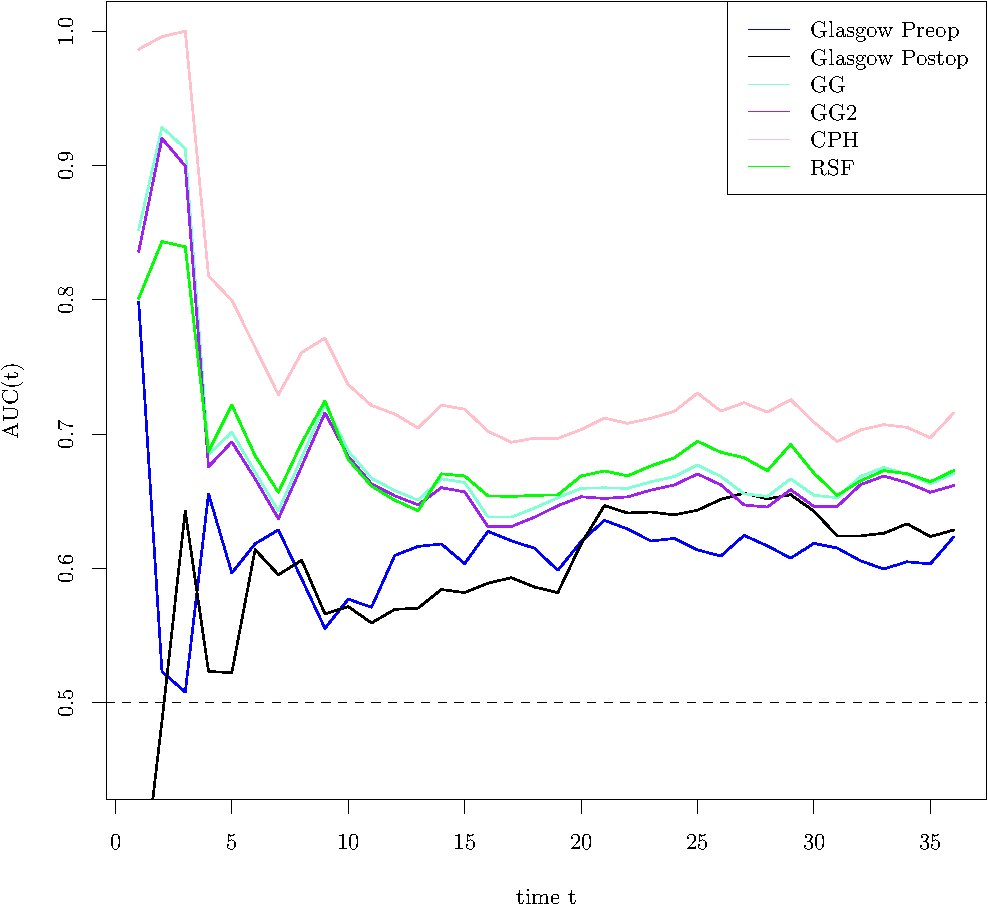
\includegraphics[width=\maxwidth]{figure/05-timeROC-1} 

}



\end{knitrout}

\begin{knitrout}
\definecolor{shadecolor}{rgb}{0.969, 0.969, 0.969}\color{fgcolor}\begin{kframe}
\begin{alltt}
\hlkwd{risksetROC}\hlstd{(data.glasgow}\hlopt{$}\hlstd{Time}\hlopt{/}\hlnum{365.25}\hlopt{*}\hlnum{12}\hlstd{,} \hlkwc{status} \hlstd{= data.glasgow}\hlopt{$}\hlstd{DSD,} \hlkwc{marker} \hlstd{= mskcc_pre.linpred.glasgow,} \hlkwc{predict.time} \hlstd{=} \hlnum{12}\hlstd{)}
\end{alltt}
\end{kframe}

{\centering 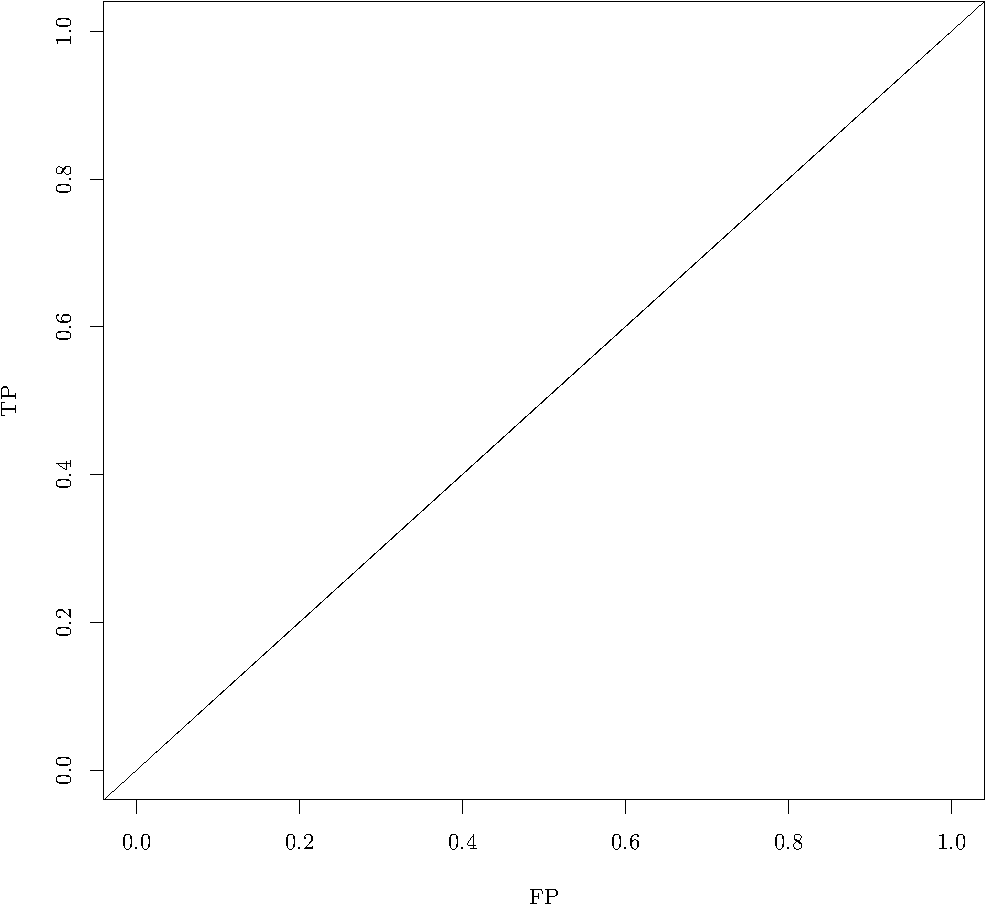
\includegraphics[width=\maxwidth]{figure/05-risksetROC-1} 

}


\begin{kframe}\begin{verbatim}
## $marker
##   [1] -0.09676 -0.08538 -0.07023 -0.07019 -0.06997 -0.06977 -0.06961
##   [8] -0.06958 -0.06955 -0.06950 -0.06947 -0.06928 -0.06917 -0.06916
##  [15] -0.06910 -0.06904 -0.06896 -0.06895 -0.06894 -0.06888 -0.06884
##  [22] -0.06884 -0.06881 -0.06876 -0.06867 -0.06867 -0.06865 -0.06864
##  [29] -0.06860 -0.06860 -0.06859 -0.06859 -0.06856 -0.06856 -0.06855
##  [36] -0.06854 -0.06852 -0.06851 -0.06851 -0.06850 -0.06848 -0.06844
##  [43] -0.06839 -0.06831 -0.06831 -0.06830 -0.06826 -0.06826 -0.06824
##  [50] -0.06823 -0.06823 -0.06823 -0.06823 -0.06823 -0.06822 -0.06821
##  [57] -0.06819 -0.06817 -0.06814 -0.06812 -0.06807 -0.06805 -0.06799
##  [64] -0.06797 -0.06797 -0.06797 -0.06790 -0.06787 -0.06787 -0.06778
##  [71] -0.06775 -0.06772 -0.06755 -0.06752 -0.06752 -0.06750 -0.06748
##  [78] -0.06748 -0.06746 -0.06744 -0.06743 -0.06743 -0.06731 -0.06725
##  [85] -0.06723 -0.06723 -0.06721 -0.06715 -0.06713 -0.06710 -0.06710
##  [92] -0.06709 -0.06704 -0.06704 -0.06703 -0.06703 -0.06703 -0.06703
##  [99] -0.06695 -0.06689 -0.06688 -0.06688 -0.06687 -0.06687 -0.06685
## [106] -0.06680 -0.06675 -0.06670 -0.06669 -0.06662 -0.06658 -0.06512
## [113] -0.06443 -0.06388 -0.06340 -0.06317 -0.06315 -0.06312 -0.06263
## [120] -0.06246 -0.06235 -0.06222 -0.06208 -0.06185
## 
## $TP
##   [1] 1.000000 0.992165 0.984240 0.976194 0.968148 0.960100 0.952051
##   [8] 0.944000 0.935949 0.927898 0.919846 0.911794 0.903741 0.895686
##  [15] 0.887632 0.879577 0.871522 0.863466 0.855409 0.847353 0.839297
##  [22] 0.831240 0.823183 0.815125 0.807068 0.799009 0.790951 0.782893
##  [29] 0.774834 0.766775 0.758716 0.750657 0.742598 0.734539 0.726480
##  [36] 0.718420 0.710361 0.702301 0.694242 0.686182 0.678122 0.670062
##  [43] 0.662002 0.653942 0.645880 0.637819 0.629758 0.621696 0.613634
##  [50] 0.605573 0.597511 0.589449 0.581387 0.573325 0.565263 0.557201
##  [57] 0.549139 0.541077 0.533014 0.524952 0.516889 0.508826 0.500762
##  [64] 0.492698 0.484635 0.476571 0.468507 0.460442 0.452377 0.444312
##  [71] 0.436247 0.428181 0.420115 0.412048 0.403980 0.395912 0.387845
##  [78] 0.379777 0.371709 0.363641 0.355572 0.347504 0.339436 0.331366
##  [85] 0.323296 0.315226 0.307156 0.299086 0.291016 0.282945 0.274874
##  [92] 0.266803 0.258732 0.250660 0.242589 0.234517 0.226446 0.218374
##  [99] 0.210303 0.202230 0.194158 0.186085 0.178012 0.169939 0.161866
## [106] 0.153793 0.145720 0.137646 0.129572 0.121498 0.113423 0.105347
## [113] 0.097260 0.089168 0.081071 0.072970 0.064867 0.056764 0.048661
## [120] 0.040554 0.032445 0.024336 0.016225 0.008114 0.000000 0.000000
## 
## $FP
##   [1] 1.000000 0.991935 0.983871 0.975806 0.967742 0.959677 0.951613
##   [8] 0.943548 0.935484 0.927419 0.919355 0.911290 0.903226 0.895161
##  [15] 0.887097 0.879032 0.870968 0.862903 0.854839 0.846774 0.838710
##  [22] 0.830645 0.822581 0.814516 0.806452 0.798387 0.790323 0.782258
##  [29] 0.774194 0.766129 0.758065 0.750000 0.741935 0.733871 0.725806
##  [36] 0.717742 0.709677 0.701613 0.693548 0.685484 0.677419 0.669355
##  [43] 0.661290 0.653226 0.645161 0.637097 0.629032 0.620968 0.612903
##  [50] 0.604839 0.596774 0.588710 0.580645 0.572581 0.564516 0.556452
##  [57] 0.548387 0.540323 0.532258 0.524194 0.516129 0.508065 0.500000
##  [64] 0.491935 0.483871 0.475806 0.467742 0.459677 0.451613 0.443548
##  [71] 0.435484 0.427419 0.419355 0.411290 0.403226 0.395161 0.387097
##  [78] 0.379032 0.370968 0.362903 0.354839 0.346774 0.338710 0.330645
##  [85] 0.322581 0.314516 0.306452 0.298387 0.290323 0.282258 0.274194
##  [92] 0.266129 0.258065 0.250000 0.241935 0.233871 0.225806 0.217742
##  [99] 0.209677 0.201613 0.193548 0.185484 0.177419 0.169355 0.161290
## [106] 0.153226 0.145161 0.137097 0.129032 0.120968 0.112903 0.104839
## [113] 0.096774 0.088710 0.080645 0.072581 0.064516 0.056452 0.048387
## [120] 0.040323 0.032258 0.024194 0.016129 0.008065 0.000000 0.000000
## 
## $AUC
## [1] 0.5006
\end{verbatim}
\begin{alltt}
\hlkwd{risksetROC}\hlstd{(data.glasgow}\hlopt{$}\hlstd{Time}\hlopt{/}\hlnum{365.25}\hlopt{*}\hlnum{12}\hlstd{,} \hlkwc{status} \hlstd{= data.glasgow}\hlopt{$}\hlstd{DSD,} \hlkwc{marker} \hlstd{= mskcc_post.linpred.glasgow,} \hlkwc{predict.time} \hlstd{=} \hlnum{12}\hlstd{)}
\end{alltt}
\end{kframe}

{\centering 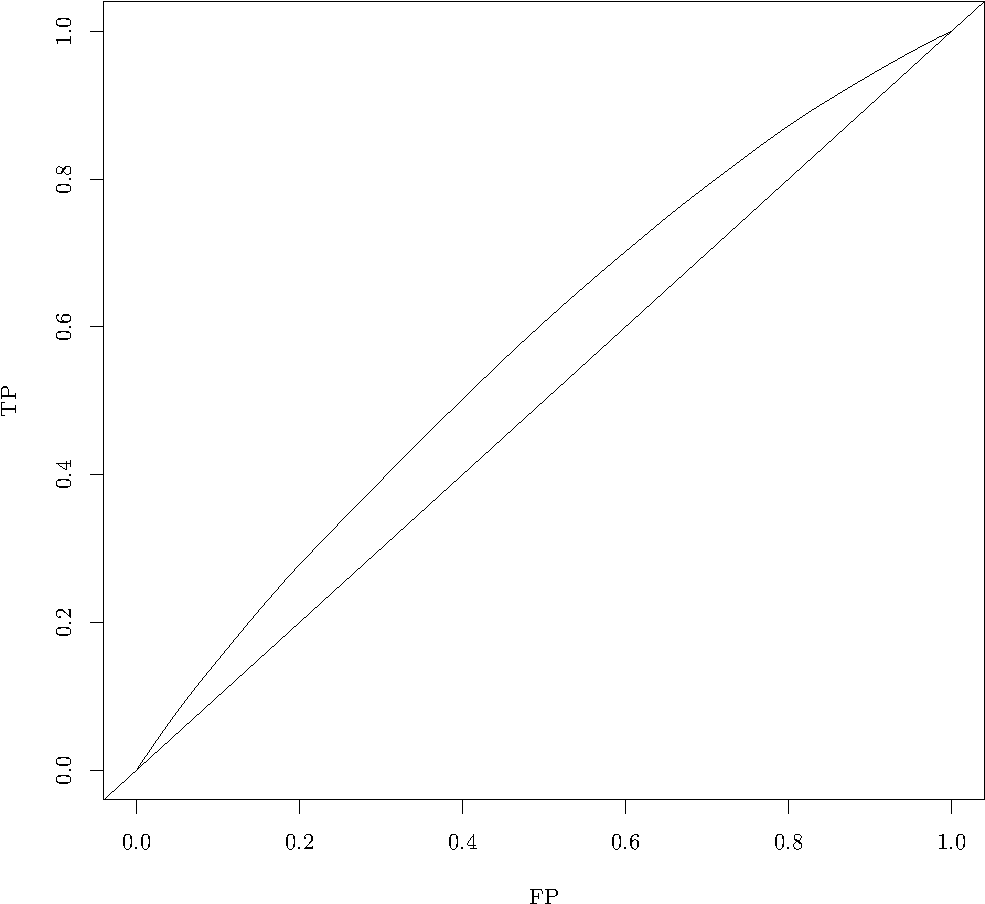
\includegraphics[width=\maxwidth]{figure/05-risksetROC-2} 

}


\begin{kframe}\begin{verbatim}
## $marker
##   [1] 1.734 1.808 1.847 1.877 1.890 1.899 1.901 1.933 1.945 1.953 1.955
##  [12] 1.980 1.984 1.990 2.001 2.009 2.009 2.012 2.016 2.032 2.033 2.086
##  [23] 2.099 2.113 2.136 2.152 2.165 2.182 2.208 2.210 2.224 2.225 2.227
##  [34] 2.229 2.233 2.240 2.245 2.248 2.252 2.259 2.261 2.286 2.295 2.320
##  [45] 2.324 2.331 2.335 2.337 2.341 2.341 2.342 2.347 2.348 2.355 2.379
##  [56] 2.379 2.382 2.384 2.388 2.403 2.404 2.415 2.425 2.426 2.427 2.437
##  [67] 2.451 2.464 2.471 2.474 2.477 2.481 2.485 2.491 2.493 2.495 2.496
##  [78] 2.499 2.515 2.515 2.515 2.521 2.524 2.524 2.527 2.527 2.529 2.531
##  [89] 2.533 2.538 2.541 2.545 2.548 2.548 2.555 2.558 2.564 2.567 2.572
## [100] 2.572 2.604 2.650 2.656 2.656 2.669 2.679 2.685 2.710 2.711 2.714
## [111] 2.717 2.718 2.721 2.726 2.742 2.766 2.779 2.806 2.850 2.860 2.883
## [122] 2.884 2.895 2.938
## 
## $TP
##   [1] 1.00000 0.99594 0.99156 0.98701 0.98232 0.97757 0.97278 0.96798
##   [9] 0.96302 0.95801 0.95295 0.94788 0.94269 0.93747 0.93222 0.92691
##  [17] 0.92156 0.91621 0.91085 0.90546 0.89999 0.89451 0.88873 0.88288
##  [25] 0.87695 0.87087 0.86471 0.85845 0.85209 0.84557 0.83903 0.83240
##  [33] 0.82576 0.81911 0.81244 0.80575 0.79901 0.79224 0.78544 0.77862
##  [41] 0.77175 0.76487 0.75782 0.75070 0.74340 0.73607 0.72869 0.72127
##  [49] 0.71385 0.70640 0.69894 0.69148 0.68398 0.67648 0.66892 0.66118
##  [57] 0.65343 0.64566 0.63788 0.63007 0.62214 0.61419 0.60616 0.59806
##  [65] 0.58994 0.58181 0.57361 0.56529 0.55686 0.54837 0.53986 0.53132
##  [73] 0.52275 0.51413 0.50547 0.49679 0.48810 0.47939 0.47066 0.46179
##  [81] 0.45292 0.44405 0.43513 0.42618 0.41723 0.40825 0.39927 0.39027
##  [89] 0.38126 0.37223 0.36315 0.35404 0.34490 0.33573 0.32657 0.31734
##  [97] 0.30808 0.29875 0.28940 0.28001 0.27062 0.26092 0.25077 0.24056
## [105] 0.23035 0.22000 0.20955 0.19903 0.18825 0.17745 0.16663 0.15577
## [113] 0.14490 0.13400 0.12305 0.11191 0.10051 0.08895 0.07709 0.06469
## [121] 0.05217 0.03935 0.02651 0.01354 0.00000 0.00000
## 
## $FP
##   [1] 1.000000 0.991935 0.983871 0.975806 0.967742 0.959677 0.951613
##   [8] 0.943548 0.935484 0.927419 0.919355 0.911290 0.903226 0.895161
##  [15] 0.887097 0.879032 0.870968 0.862903 0.854839 0.846774 0.838710
##  [22] 0.830645 0.822581 0.814516 0.806452 0.798387 0.790323 0.782258
##  [29] 0.774194 0.766129 0.758065 0.750000 0.741935 0.733871 0.725806
##  [36] 0.717742 0.709677 0.701613 0.693548 0.685484 0.677419 0.669355
##  [43] 0.661290 0.653226 0.645161 0.637097 0.629032 0.620968 0.612903
##  [50] 0.604839 0.596774 0.588710 0.580645 0.572581 0.564516 0.556452
##  [57] 0.548387 0.540323 0.532258 0.524194 0.516129 0.508065 0.500000
##  [64] 0.491935 0.483871 0.475806 0.467742 0.459677 0.451613 0.443548
##  [71] 0.435484 0.427419 0.419355 0.411290 0.403226 0.395161 0.387097
##  [78] 0.379032 0.370968 0.362903 0.354839 0.346774 0.338710 0.330645
##  [85] 0.322581 0.314516 0.306452 0.298387 0.290323 0.282258 0.274194
##  [92] 0.266129 0.258065 0.250000 0.241935 0.233871 0.225806 0.217742
##  [99] 0.209677 0.201613 0.193548 0.185484 0.177419 0.169355 0.161290
## [106] 0.153226 0.145161 0.137097 0.129032 0.120968 0.112903 0.104839
## [113] 0.096774 0.088710 0.080645 0.072581 0.064516 0.056452 0.048387
## [120] 0.040323 0.032258 0.024194 0.016129 0.008065 0.000000 0.000000
## 
## $AUC
## [1] 0.5743
\end{verbatim}
\begin{alltt}
\hlkwd{risksetROC}\hlstd{(data.glasgow}\hlopt{$}\hlstd{Time}\hlopt{/}\hlnum{365.25}\hlopt{*}\hlnum{12}\hlstd{,} \hlkwc{status} \hlstd{= data.glasgow}\hlopt{$}\hlstd{DSD,} \hlkwc{marker} \hlstd{= gg.linpred.glasgow,} \hlkwc{predict.time} \hlstd{=} \hlnum{12}\hlstd{)}
\end{alltt}
\end{kframe}

{\centering 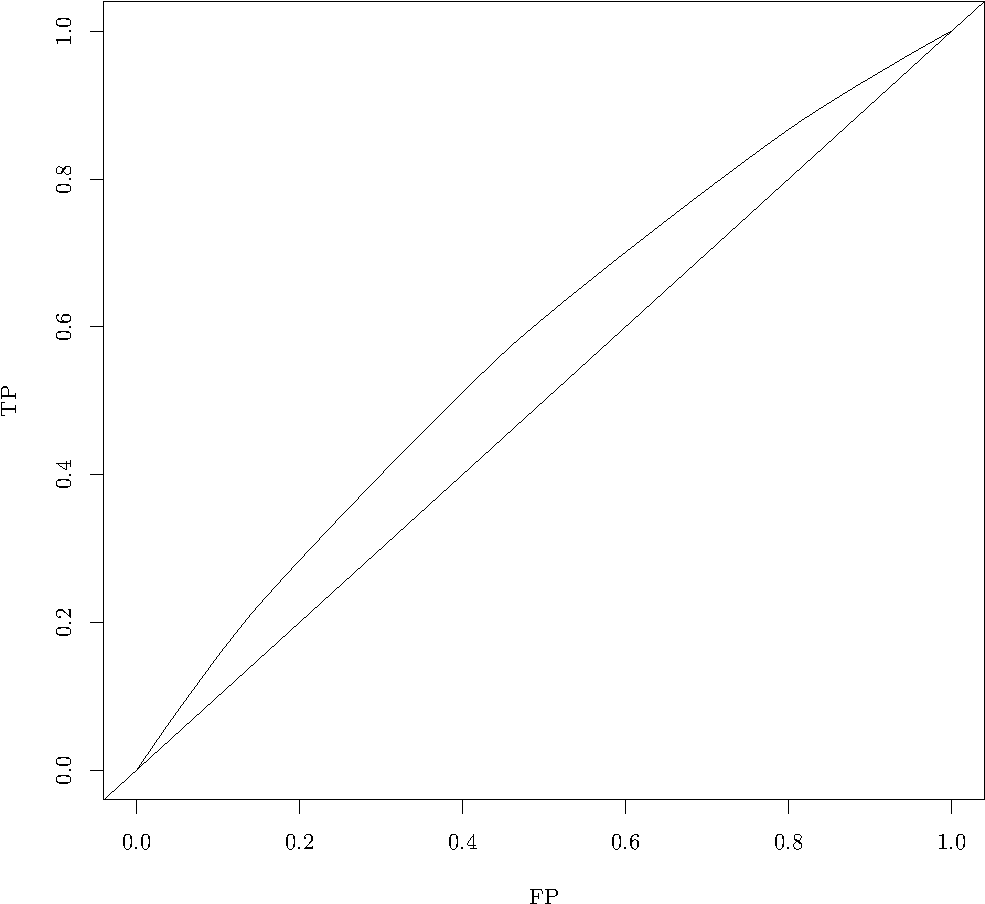
\includegraphics[width=\maxwidth]{figure/05-risksetROC-3} 

}


\begin{kframe}\begin{verbatim}
## $marker
##   [1] -0.50102 -0.38477 -0.35377 -0.35377 -0.35377 -0.34602 -0.34602
##   [8] -0.30727 -0.30727 -0.30727 -0.30727 -0.30727 -0.30727 -0.30727
##  [15] -0.26852 -0.26852 -0.25302 -0.22977 -0.22977 -0.22977 -0.22977
##  [22] -0.22091 -0.19102 -0.14341 -0.14341 -0.11625 -0.11625 -0.11351
##  [29] -0.10466 -0.10075 -0.08916 -0.07750 -0.07750 -0.06591 -0.06591
##  [36] -0.06591 -0.06591 -0.05816 -0.03875 -0.03875 -0.03875 -0.03875
##  [43] -0.03100 -0.02716 -0.02716 -0.02716 -0.02716 -0.02716 -0.01941
##  [50] -0.01550 -0.01166  0.00000  0.00000  0.00000  0.00000  0.00775
##  [57]  0.01159  0.01159  0.01159  0.03875  0.03875  0.03875  0.03875
##  [64]  0.08910  0.08910  0.12785  0.12785  0.17050  0.18711  0.18711
##  [71]  0.19486  0.20261  0.20261  0.20261  0.23361  0.23659  0.24136
##  [78]  0.24136  0.24136  0.24136  0.26461  0.26648  0.28011  0.28011
##  [85]  0.28011  0.28011  0.28011  0.28011  0.28011  0.29084  0.31409
##  [92]  0.31409  0.31886  0.34125  0.35284  0.35284  0.35761  0.35761
##  [99]  0.35761  0.36450  0.39159  0.39159  0.39159  0.39159  0.43034
## [106]  0.43512  0.46909  0.51262  0.53500  0.54386  0.54386  0.57486
## [113]  0.61361  0.62136  0.62136  0.62136  0.62136  0.64461  0.66011
## [120]  0.66011  0.69886  0.69886  0.69886  0.69886
## 
## $TP
##   [1] 1.00000 0.99584 0.99117 0.98636 0.98154 0.97672 0.97187 0.96702
##   [9] 0.96197 0.95692 0.95188 0.94683 0.94179 0.93674 0.93170 0.92645
##  [17] 0.92120 0.91588 0.91043 0.90497 0.89952 0.89407 0.88857 0.88290
##  [25] 0.87696 0.87101 0.86490 0.85880 0.85267 0.84649 0.84029 0.83401
##  [33] 0.82766 0.82131 0.81489 0.80847 0.80204 0.79562 0.78915 0.78255
##  [41] 0.77595 0.76935 0.76275 0.75610 0.74942 0.74274 0.73607 0.72939
##  [49] 0.72271 0.71598 0.70923 0.70245 0.69559 0.68872 0.68186 0.67500
##  [57] 0.66809 0.66115 0.65421 0.64727 0.64013 0.63300 0.62587 0.61874
##  [65] 0.61124 0.60374 0.59594 0.58815 0.58001 0.57174 0.56346 0.55513
##  [73] 0.54673 0.53832 0.52992 0.52126 0.51256 0.50383 0.49510 0.48636
##  [81] 0.47763 0.46869 0.45973 0.45066 0.44158 0.43250 0.42342 0.41434
##  [89] 0.40526 0.39618 0.38701 0.37761 0.36822 0.35878 0.34913 0.33937
##  [97] 0.32960 0.31979 0.30998 0.30017 0.29030 0.28015 0.27000 0.25985
## [105] 0.24970 0.23915 0.22855 0.21758 0.20612 0.19441 0.18259 0.17077
## [113] 0.15858 0.14591 0.13314 0.12037 0.10760 0.09482 0.08175 0.06848
## [121] 0.05520 0.04140 0.02760 0.01380 0.00000 0.00000
## 
## $FP
##   [1] 1.000000 0.991935 0.983871 0.975806 0.967742 0.959677 0.951613
##   [8] 0.943548 0.935484 0.927419 0.919355 0.911290 0.903226 0.895161
##  [15] 0.887097 0.879032 0.870968 0.862903 0.854839 0.846774 0.838710
##  [22] 0.830645 0.822581 0.814516 0.806452 0.798387 0.790323 0.782258
##  [29] 0.774194 0.766129 0.758065 0.750000 0.741935 0.733871 0.725806
##  [36] 0.717742 0.709677 0.701613 0.693548 0.685484 0.677419 0.669355
##  [43] 0.661290 0.653226 0.645161 0.637097 0.629032 0.620968 0.612903
##  [50] 0.604839 0.596774 0.588710 0.580645 0.572581 0.564516 0.556452
##  [57] 0.548387 0.540323 0.532258 0.524194 0.516129 0.508065 0.500000
##  [64] 0.491935 0.483871 0.475806 0.467742 0.459677 0.451613 0.443548
##  [71] 0.435484 0.427419 0.419355 0.411290 0.403226 0.395161 0.387097
##  [78] 0.379032 0.370968 0.362903 0.354839 0.346774 0.338710 0.330645
##  [85] 0.322581 0.314516 0.306452 0.298387 0.290323 0.282258 0.274194
##  [92] 0.266129 0.258065 0.250000 0.241935 0.233871 0.225806 0.217742
##  [99] 0.209677 0.201613 0.193548 0.185484 0.177419 0.169355 0.161290
## [106] 0.153226 0.145161 0.137097 0.129032 0.120968 0.112903 0.104839
## [113] 0.096774 0.088710 0.080645 0.072581 0.064516 0.056452 0.048387
## [120] 0.040323 0.032258 0.024194 0.016129 0.008065 0.000000 0.000000
## 
## $AUC
## [1] 0.5858
\end{verbatim}
\begin{alltt}
\hlkwd{risksetROC}\hlstd{(data.glasgow}\hlopt{$}\hlstd{Time}\hlopt{/}\hlnum{365.25}\hlopt{*}\hlnum{12}\hlstd{,} \hlkwc{status} \hlstd{= data.glasgow}\hlopt{$}\hlstd{DSD,} \hlkwc{marker} \hlstd{= gg2.linpred.glasgow,} \hlkwc{predict.time} \hlstd{=} \hlnum{12}\hlstd{)}
\end{alltt}
\end{kframe}

{\centering 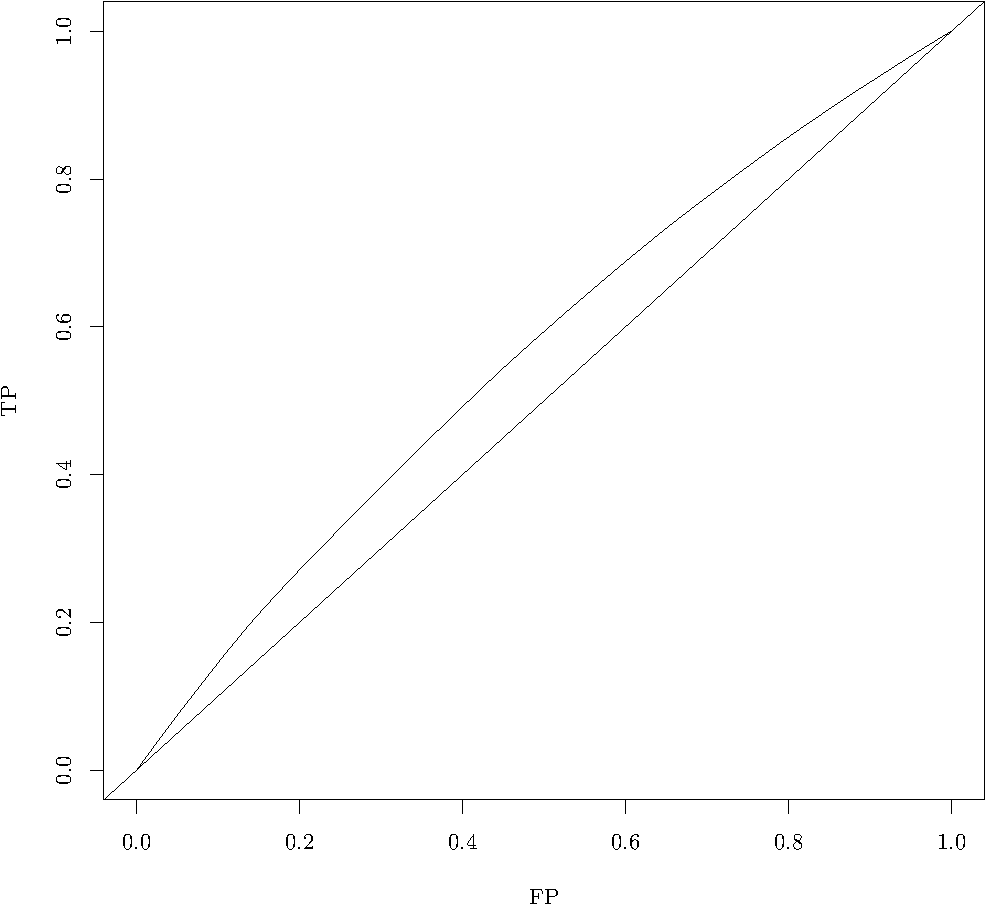
\includegraphics[width=\maxwidth]{figure/05-risksetROC-4} 

}


\begin{kframe}\begin{verbatim}
## $marker
##   [1] -0.508607 -0.395314 -0.365103 -0.365103 -0.365103 -0.357550 -0.357550
##   [8] -0.319786 -0.319786 -0.319786 -0.319786 -0.319786 -0.319786 -0.319786
##  [15] -0.282022 -0.282022 -0.272976 -0.266916 -0.244258 -0.244258 -0.244258
##  [22] -0.244258 -0.206494 -0.197448 -0.197448 -0.159684 -0.144578 -0.130965
##  [29] -0.121919 -0.121919 -0.121919 -0.121919 -0.114367 -0.113292 -0.113292
##  [36] -0.098187 -0.084155 -0.084155 -0.084155 -0.084155 -0.084155 -0.076602
##  [43] -0.075528 -0.075528 -0.069050 -0.046391 -0.046391 -0.046391 -0.037764
##  [50] -0.037764 -0.037764 -0.037764 -0.030211 -0.015106  0.000000  0.000000
##  [57]  0.000000  0.000000  0.007553  0.029137  0.029137  0.037764  0.037764
##  [64]  0.037764  0.037764  0.066901  0.066901  0.144997  0.144997  0.152550
##  [71]  0.160103  0.160103  0.160103  0.164872  0.166162  0.190314  0.197867
##  [78]  0.197867  0.197867  0.197867  0.217742  0.220525  0.231354  0.235631
##  [85]  0.235631  0.235631  0.235631  0.235631  0.235631  0.235631  0.240400
##  [92]  0.240400  0.273395  0.278164  0.278164  0.311159  0.311159  0.311159
##  [99]  0.315928  0.315928  0.315928  0.315928  0.324555  0.347214  0.353693
## [106]  0.386688  0.391457  0.462216  0.484658  0.484658  0.513376  0.514869
## [113]  0.552633  0.560186  0.560186  0.560186  0.560186  0.582845  0.597950
## [120]  0.597950  0.635714  0.635714  0.635714  0.635714
## 
## $TP
##   [1] 1.00000 0.99570 0.99088 0.98591 0.98094 0.97597 0.97097 0.96596
##   [9] 0.96077 0.95557 0.95037 0.94517 0.93998 0.93478 0.92958 0.92418
##  [17] 0.91878 0.91334 0.90786 0.90225 0.89665 0.89104 0.88544 0.87961
##  [25] 0.87374 0.86787 0.86177 0.85557 0.84929 0.84296 0.83662 0.83029
##  [33] 0.82395 0.81757 0.81118 0.80479 0.79830 0.79173 0.78515 0.77857
##  [41] 0.77199 0.76541 0.75878 0.75215 0.74551 0.73883 0.73200 0.72517
##  [49] 0.71833 0.71144 0.70455 0.69766 0.69077 0.68383 0.67678 0.66962
##  [57] 0.66246 0.65531 0.64815 0.64094 0.63357 0.62620 0.61877 0.61134
##  [65] 0.60391 0.59648 0.58883 0.58117 0.57290 0.56463 0.55629 0.54789
##  [73] 0.53949 0.53109 0.52266 0.51421 0.50555 0.49683 0.48810 0.47938
##  [81] 0.47066 0.46176 0.45284 0.44382 0.43476 0.42570 0.41665 0.40759
##  [89] 0.39853 0.38947 0.38041 0.37131 0.36221 0.35281 0.34335 0.33390
##  [97] 0.32413 0.31437 0.30460 0.29478 0.28497 0.27515 0.26534 0.25544
## [105] 0.24531 0.23512 0.22458 0.21399 0.20263 0.19101 0.17939 0.16744
## [113] 0.15546 0.14302 0.13049 0.11796 0.10543 0.09290 0.08008 0.06707
## [121] 0.05406 0.04054 0.02703 0.01351 0.00000 0.00000
## 
## $FP
##   [1] 1.000000 0.991935 0.983871 0.975806 0.967742 0.959677 0.951613
##   [8] 0.943548 0.935484 0.927419 0.919355 0.911290 0.903226 0.895161
##  [15] 0.887097 0.879032 0.870968 0.862903 0.854839 0.846774 0.838710
##  [22] 0.830645 0.822581 0.814516 0.806452 0.798387 0.790323 0.782258
##  [29] 0.774194 0.766129 0.758065 0.750000 0.741935 0.733871 0.725806
##  [36] 0.717742 0.709677 0.701613 0.693548 0.685484 0.677419 0.669355
##  [43] 0.661290 0.653226 0.645161 0.637097 0.629032 0.620968 0.612903
##  [50] 0.604839 0.596774 0.588710 0.580645 0.572581 0.564516 0.556452
##  [57] 0.548387 0.540323 0.532258 0.524194 0.516129 0.508065 0.500000
##  [64] 0.491935 0.483871 0.475806 0.467742 0.459677 0.451613 0.443548
##  [71] 0.435484 0.427419 0.419355 0.411290 0.403226 0.395161 0.387097
##  [78] 0.379032 0.370968 0.362903 0.354839 0.346774 0.338710 0.330645
##  [85] 0.322581 0.314516 0.306452 0.298387 0.290323 0.282258 0.274194
##  [92] 0.266129 0.258065 0.250000 0.241935 0.233871 0.225806 0.217742
##  [99] 0.209677 0.201613 0.193548 0.185484 0.177419 0.169355 0.161290
## [106] 0.153226 0.145161 0.137097 0.129032 0.120968 0.112903 0.104839
## [113] 0.096774 0.088710 0.080645 0.072581 0.064516 0.056452 0.048387
## [120] 0.040323 0.032258 0.024194 0.016129 0.008065 0.000000 0.000000
## 
## $AUC
## [1] 0.5815
\end{verbatim}
\begin{alltt}
\hlkwd{risksetROC}\hlstd{(data.glasgow}\hlopt{$}\hlstd{Time}\hlopt{/}\hlnum{365.25}\hlopt{*}\hlnum{12}\hlstd{,} \hlkwc{status} \hlstd{= data.glasgow}\hlopt{$}\hlstd{DSD,} \hlkwc{marker} \hlstd{= cph.linpred.glasgow,} \hlkwc{predict.time} \hlstd{=} \hlnum{12}\hlstd{)}
\end{alltt}
\end{kframe}

{\centering 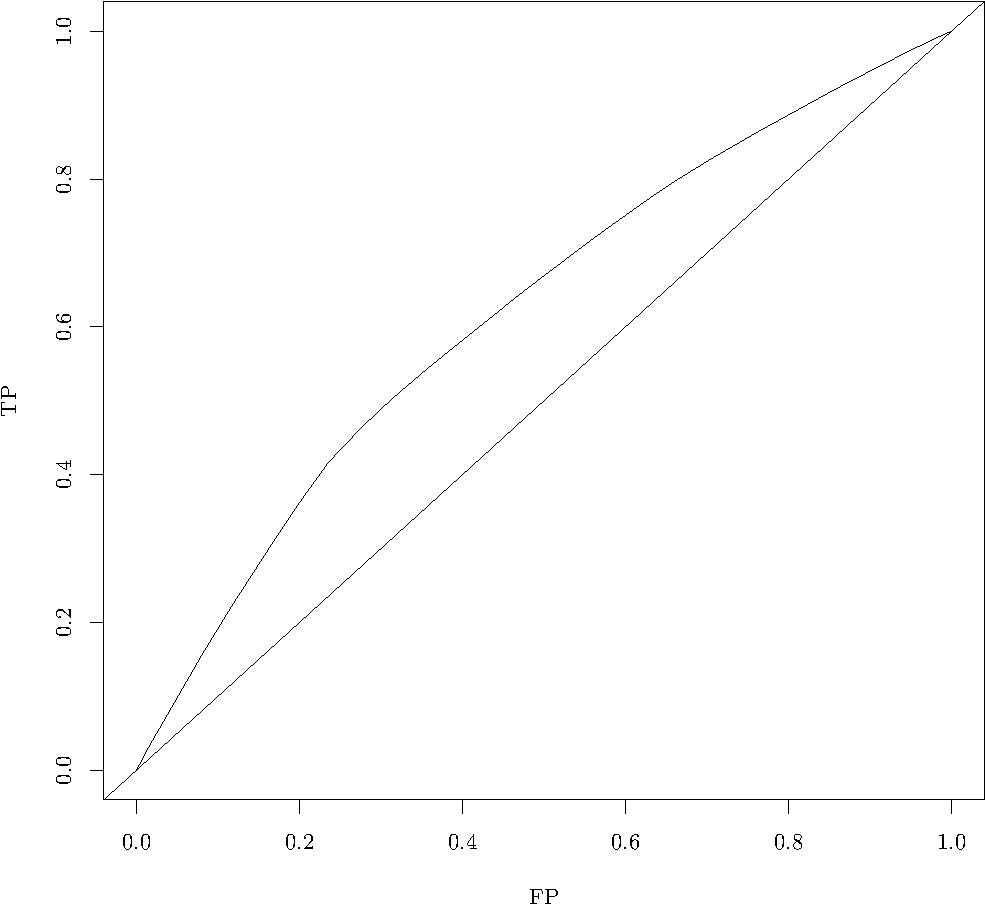
\includegraphics[width=\maxwidth]{figure/05-risksetROC-5} 

}


\begin{kframe}\begin{verbatim}
## $marker
##   [1] -0.28807 -0.17284 -0.17284 -0.14979 -0.11523 -0.11523 -0.11523
##   [8] -0.06914 -0.06914 -0.06914 -0.05761 -0.05761 -0.05761 -0.05761
##  [15] -0.05761 -0.05761 -0.04609 -0.02305  0.00000  0.00000  0.00000
##  [22]  0.00000  0.00000  0.00000  0.00000  0.00000  0.00000  0.00000
##  [29]  0.00000  0.01152  0.05761  0.05761  0.05761  0.05761  0.05761
##  [36]  0.05761  0.08066  0.09166  0.11523  0.11523  0.11523  0.11523
##  [43]  0.17284  0.20689  0.20689  0.24146  0.24146  0.25298  0.25350
##  [50]  0.26450  0.26450  0.26450  0.26450  0.28755  0.28807  0.31060
##  [57]  0.32212  0.32212  0.32212  0.32212  0.32212  0.32212  0.32212
##  [64]  0.32212  0.33364  0.35669  0.37973  0.37973  0.37973  0.37973
##  [71]  0.37973  0.37973  0.37973  0.37973  0.37973  0.37973  0.37973
##  [78]  0.37973  0.39125  0.40278  0.43734  0.43734  0.43734  0.43734
##  [85]  0.49496  0.49496  0.49496  0.55257  0.55257  0.61019  0.61019
##  [92]  0.61019  0.65364  0.68821  0.72541  0.91814  0.91814  0.91814
##  [99]  0.94171  0.96423  0.99880  0.99932  1.02185  1.03337  1.03337
## [106]  1.03337  1.03337  1.03337  1.03337  1.06794  1.09098  1.09098
## [113]  1.09098  1.09098  1.14860  1.14860  1.14860  1.14860  1.14860
## [120]  1.14860  1.14860  1.14860  1.20621  1.26382
## 
## $TP
##   [1] 1.00000 0.99634 0.99222 0.98811 0.98390 0.97955 0.97519 0.97084
##   [9] 0.96627 0.96171 0.95715 0.95254 0.94792 0.94331 0.93869 0.93408
##  [17] 0.92947 0.92480 0.92002 0.91513 0.91025 0.90536 0.90047 0.89558
##  [25] 0.89069 0.88581 0.88092 0.87603 0.87114 0.86626 0.86131 0.85613
##  [33] 0.85096 0.84578 0.84060 0.83542 0.83024 0.82495 0.81959 0.81410
##  [41] 0.80862 0.80313 0.79765 0.79184 0.78583 0.77982 0.77359 0.76737
##  [49] 0.76108 0.75478 0.74841 0.74204 0.73567 0.72931 0.72279 0.71627
##  [57] 0.70960 0.70286 0.69611 0.68937 0.68262 0.67588 0.66913 0.66238
##  [65] 0.65564 0.64882 0.64183 0.63469 0.62754 0.62040 0.61325 0.60610
##  [73] 0.59896 0.59181 0.58467 0.57752 0.57038 0.56323 0.55609 0.54886
##  [81] 0.54155 0.53398 0.52641 0.51884 0.51127 0.50325 0.49523 0.48721
##  [89] 0.47872 0.47023 0.46123 0.45223 0.44323 0.43384 0.42411 0.41401
##  [97] 0.40177 0.38953 0.37729 0.36475 0.35193 0.33866 0.32538 0.31180
## [105] 0.29807 0.28433 0.27059 0.25685 0.24312 0.22938 0.21516 0.20061
## [113] 0.18605 0.17150 0.15695 0.14153 0.12612 0.11070 0.09529 0.07987
## [121] 0.06446 0.04904 0.03363 0.01730 0.00000 0.00000
## 
## $FP
##   [1] 1.000000 0.991935 0.983871 0.975806 0.967742 0.959677 0.951613
##   [8] 0.943548 0.935484 0.927419 0.919355 0.911290 0.903226 0.895161
##  [15] 0.887097 0.879032 0.870968 0.862903 0.854839 0.846774 0.838710
##  [22] 0.830645 0.822581 0.814516 0.806452 0.798387 0.790323 0.782258
##  [29] 0.774194 0.766129 0.758065 0.750000 0.741935 0.733871 0.725806
##  [36] 0.717742 0.709677 0.701613 0.693548 0.685484 0.677419 0.669355
##  [43] 0.661290 0.653226 0.645161 0.637097 0.629032 0.620968 0.612903
##  [50] 0.604839 0.596774 0.588710 0.580645 0.572581 0.564516 0.556452
##  [57] 0.548387 0.540323 0.532258 0.524194 0.516129 0.508065 0.500000
##  [64] 0.491935 0.483871 0.475806 0.467742 0.459677 0.451613 0.443548
##  [71] 0.435484 0.427419 0.419355 0.411290 0.403226 0.395161 0.387097
##  [78] 0.379032 0.370968 0.362903 0.354839 0.346774 0.338710 0.330645
##  [85] 0.322581 0.314516 0.306452 0.298387 0.290323 0.282258 0.274194
##  [92] 0.266129 0.258065 0.250000 0.241935 0.233871 0.225806 0.217742
##  [99] 0.209677 0.201613 0.193548 0.185484 0.177419 0.169355 0.161290
## [106] 0.153226 0.145161 0.137097 0.129032 0.120968 0.112903 0.104839
## [113] 0.096774 0.088710 0.080645 0.072581 0.064516 0.056452 0.048387
## [120] 0.040323 0.032258 0.024194 0.016129 0.008065 0.000000 0.000000
## 
## $AUC
## [1] 0.6215
\end{verbatim}
\begin{alltt}
\hlkwd{risksetROC}\hlstd{(data.glasgow}\hlopt{$}\hlstd{Time}\hlopt{/}\hlnum{365.25}\hlopt{*}\hlnum{12}\hlstd{,} \hlkwc{status} \hlstd{= data.glasgow}\hlopt{$}\hlstd{DSD,} \hlkwc{marker} \hlstd{= rsf.linpred.glasgow,} \hlkwc{predict.time} \hlstd{=} \hlnum{12}\hlstd{)}
\end{alltt}
\end{kframe}

{\centering 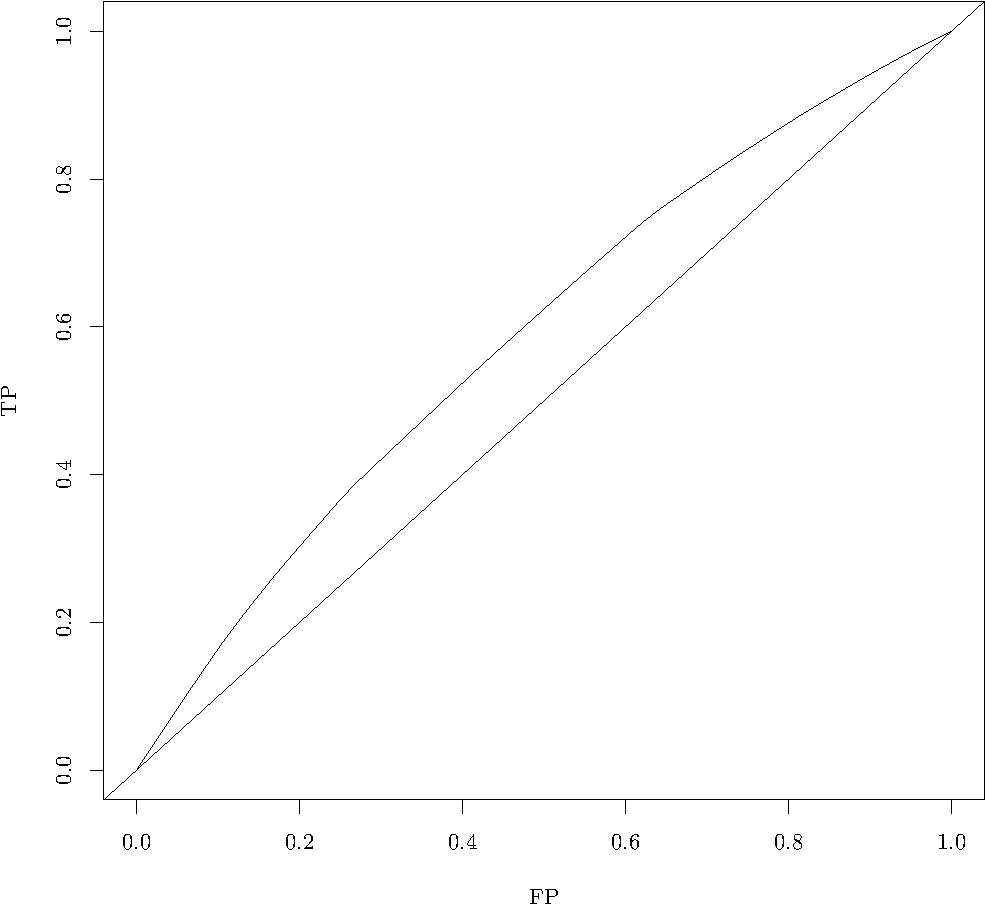
\includegraphics[width=\maxwidth]{figure/05-risksetROC-6} 

}


\begin{kframe}\begin{verbatim}
## $marker
##   [1] -2.1577 -2.1537 -2.1530 -2.1121 -2.1098 -2.0627 -2.0499 -2.0478
##   [9] -2.0373 -2.0360 -2.0360 -2.0240 -1.9944 -1.9856 -1.9788 -1.9738
##  [17] -1.9726 -1.9667 -1.9659 -1.9648 -1.9560 -1.9471 -1.9188 -1.9079
##  [25] -1.8852 -1.8844 -1.8842 -1.8828 -1.8828 -1.8797 -1.8751 -1.8586
##  [33] -1.8498 -1.8468 -1.8450 -1.8187 -1.8142 -1.8135 -1.8129 -1.8123
##  [41] -1.8121 -1.8121 -1.8101 -1.7773 -1.7518 -1.6846 -1.6826 -1.6050
##  [49] -1.5822 -1.5722 -1.5711 -1.5697 -1.5694 -1.5689 -1.5682 -1.5616
##  [57] -1.5610 -1.5580 -1.5571 -1.5538 -1.5509 -1.5507 -1.5504 -1.5500
##  [65] -1.5492 -1.5469 -1.5431 -1.5419 -1.5413 -1.5413 -1.5303 -1.5300
##  [73] -1.5171 -1.5061 -1.5048 -1.5033 -1.5031 -1.5025 -1.5020 -1.5014
##  [81] -1.5001 -1.5001 -1.5001 -1.4991 -1.4984 -1.4982 -1.4977 -1.4972
##  [89] -1.4950 -1.4892 -1.4599 -1.3967 -1.3742 -1.3034 -1.3032 -1.3029
##  [97] -1.3025 -1.2972 -1.2905 -1.2897 -1.2812 -1.2784 -1.2731 -1.2278
## [105] -1.2227 -1.2221 -1.1955 -1.1766 -1.1716 -1.1460 -1.1453 -1.0732
## [113] -1.0671 -1.0650 -1.0552 -1.0467 -1.0465 -1.0430 -1.0420 -1.0378
## [121] -1.0297 -1.0276 -1.0271 -0.9954
## 
## $TP
##   [1] 1.00000 0.99567 0.99132 0.98697 0.98243 0.97789 0.97313 0.96830
##   [9] 0.96347 0.95858 0.95369 0.94880 0.94385 0.93875 0.93360 0.92842
##  [17] 0.92322 0.91800 0.91276 0.90751 0.90226 0.89696 0.89161 0.88611
##  [25] 0.88055 0.87486 0.86917 0.86348 0.85778 0.85207 0.84635 0.84061
##  [33] 0.83477 0.82887 0.82296 0.81704 0.81096 0.80485 0.79874 0.79263
##  [41] 0.78651 0.78039 0.77427 0.76814 0.76180 0.75530 0.74835 0.74138
##  [49] 0.73386 0.72615 0.71837 0.71059 0.70279 0.69499 0.68718 0.67937
##  [57] 0.67151 0.66364 0.65575 0.64786 0.63993 0.63199 0.62404 0.61609
##  [65] 0.60814 0.60018 0.59220 0.58419 0.57617 0.56815 0.56012 0.55201
##  [73] 0.54390 0.53568 0.52737 0.51905 0.51071 0.50238 0.49404 0.48569
##  [81] 0.47734 0.46898 0.46062 0.45226 0.44389 0.43552 0.42714 0.41876
##  [89] 0.41037 0.40197 0.39352 0.38481 0.37554 0.36606 0.35588 0.34570
##  [97] 0.33552 0.32533 0.31509 0.30478 0.29446 0.28406 0.27362 0.26313
## [105] 0.25215 0.24112 0.23008 0.21874 0.20719 0.19558 0.18366 0.17174
## [113] 0.15893 0.14604 0.13312 0.12007 0.10692 0.09376 0.08055 0.06733
## [121] 0.05406 0.04068 0.02727 0.01385 0.00000 0.00000
## 
## $FP
##   [1] 1.000000 0.991935 0.983871 0.975806 0.967742 0.959677 0.951613
##   [8] 0.943548 0.935484 0.927419 0.919355 0.911290 0.903226 0.895161
##  [15] 0.887097 0.879032 0.870968 0.862903 0.854839 0.846774 0.838710
##  [22] 0.830645 0.822581 0.814516 0.806452 0.798387 0.790323 0.782258
##  [29] 0.774194 0.766129 0.758065 0.750000 0.741935 0.733871 0.725806
##  [36] 0.717742 0.709677 0.701613 0.693548 0.685484 0.677419 0.669355
##  [43] 0.661290 0.653226 0.645161 0.637097 0.629032 0.620968 0.612903
##  [50] 0.604839 0.596774 0.588710 0.580645 0.572581 0.564516 0.556452
##  [57] 0.548387 0.540323 0.532258 0.524194 0.516129 0.508065 0.500000
##  [64] 0.491935 0.483871 0.475806 0.467742 0.459677 0.451613 0.443548
##  [71] 0.435484 0.427419 0.419355 0.411290 0.403226 0.395161 0.387097
##  [78] 0.379032 0.370968 0.362903 0.354839 0.346774 0.338710 0.330645
##  [85] 0.322581 0.314516 0.306452 0.298387 0.290323 0.282258 0.274194
##  [92] 0.266129 0.258065 0.250000 0.241935 0.233871 0.225806 0.217742
##  [99] 0.209677 0.201613 0.193548 0.185484 0.177419 0.169355 0.161290
## [106] 0.153226 0.145161 0.137097 0.129032 0.120968 0.112903 0.104839
## [113] 0.096774 0.088710 0.080645 0.072581 0.064516 0.056452 0.048387
## [120] 0.040323 0.032258 0.024194 0.016129 0.008065 0.000000 0.000000
## 
## $AUC
## [1] 0.5888
\end{verbatim}
\begin{alltt}
\hlkwd{risksetAUC}\hlstd{(data.glasgow}\hlopt{$}\hlstd{Time}\hlopt{/}\hlnum{365.25}\hlopt{*}\hlnum{12}\hlstd{,} \hlkwc{status} \hlstd{= data.glasgow}\hlopt{$}\hlstd{DSD,} \hlkwc{marker} \hlstd{= mskcc_pre.linpred.glasgow,} \hlkwc{tmax} \hlstd{=} \hlnum{36}\hlstd{)}
\end{alltt}
\end{kframe}

{\centering 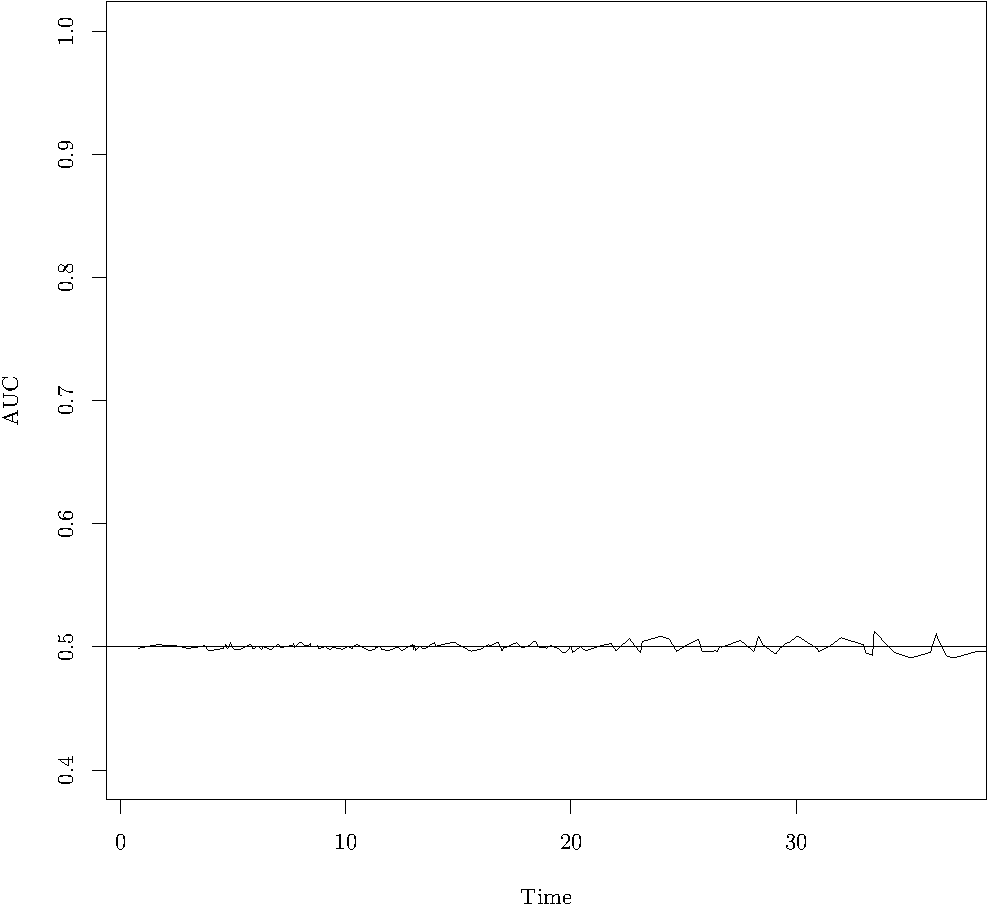
\includegraphics[width=\maxwidth]{figure/05-risksetROC-7} 

}


\begin{kframe}\begin{verbatim}
## $utimes
##   [1]   0.80   1.63   2.50   3.00   3.40   3.73   3.83   3.90   4.47   4.57
##  [11]   4.67   4.73   4.83   4.87   5.00   5.30   5.77   5.83   5.87   6.00
##  [21]   6.10   6.27   6.30   6.67   6.93   7.00   7.10   7.66   7.67   7.73
##  [31]   8.00   8.17   8.33   8.43   8.47   8.77   8.80   9.00   9.03   9.30
##  [41]   9.40   9.83  10.13  10.27  10.40  10.50  11.07  11.30  11.33  11.50
##  [51]  11.60  11.90  12.33  12.47  12.97  13.00  13.03  13.10  13.30  13.43
##  [61]  13.50  13.57  13.70  13.93  14.00  14.80  15.37  15.40  15.57  16.00
##  [71]  16.17  16.33  16.47  16.77  16.95  17.00  17.07  17.57  17.83  18.03
##  [81]  18.17  18.40  18.50  18.57  18.93  19.10  19.50  19.63  19.80  20.00
##  [91]  20.07  20.43  20.67  20.90  21.53  21.80  22.00  22.60  23.07  23.10
## [101]  23.17  24.00  24.37  24.70  25.00  25.67  25.83  26.33  26.40  26.50
## [111]  26.60  26.70  27.53  28.13  28.33  28.53  29.03  29.10  29.27  29.60
## [121]  29.67  30.07  30.97  31.00  31.53  32.00  33.00  33.10  33.40  33.47
## [131]  34.37  35.10  35.97  36.23  36.30  36.67  37.00  38.00  39.60  41.23
## [141]  43.07  45.37  46.67  47.43  47.73  48.00  49.00  51.00  54.90  59.00
## [151]  63.13  65.00  67.00  70.00  77.00  85.00  85.80  90.33  93.00  94.77
## [161] 116.00
## 
## $St
##   [1] 0.99476 0.98930 0.98383 0.97834 0.97284 0.96734 0.96185 0.95086
##   [9] 0.93986 0.93437 0.92887 0.92337 0.91788 0.90689 0.89589 0.89040
##  [17] 0.88490 0.87940 0.87391 0.86841 0.86291 0.85742 0.85192 0.84643
##  [25] 0.84093 0.83543 0.82994 0.82444 0.81894 0.81345 0.80246 0.79696
##  [33] 0.79146 0.78597 0.78047 0.77497 0.76948 0.76398 0.75845 0.75291
##  [41] 0.74737 0.74184 0.73630 0.73077 0.72523 0.71969 0.71416 0.70862
##  [49] 0.70308 0.69755 0.69201 0.68648 0.68094 0.67540 0.66987 0.66433
##  [57] 0.65880 0.65326 0.64772 0.64219 0.63665 0.63112 0.62558 0.62004
##  [65] 0.61451 0.60892 0.60333 0.59775 0.59216 0.58658 0.58099 0.57540
##  [73] 0.56982 0.56423 0.55864 0.55306 0.54747 0.54188 0.53630 0.53071
##  [81] 0.52512 0.51954 0.51395 0.50837 0.50278 0.49719 0.49161 0.48602
##  [89] 0.48043 0.46926 0.46367 0.45809 0.45250 0.44691 0.44133 0.43574
##  [97] 0.43016 0.42457 0.41898 0.41340 0.40781 0.39664 0.39105 0.38546
## [105] 0.37429 0.36870 0.36312 0.35753 0.35195 0.34636 0.34077 0.33519
## [113] 0.32960 0.32401 0.31843 0.31284 0.30725 0.30167 0.29608 0.29049
## [121] 0.28491 0.27932 0.27374 0.26815 0.26256 0.25698 0.25139 0.24580
## [129] 0.24022 0.23463 0.22904 0.22332 0.21759 0.21187 0.20614 0.20041
## [137] 0.19469 0.18289 0.17679 0.17048 0.16416 0.15760 0.15103 0.14446
## [145] 0.13790 0.13133 0.12442 0.11751 0.10967 0.10184 0.09401 0.08617
## [153] 0.07834 0.07050 0.06169 0.05141 0.04113 0.03085 0.02056 0.01028
## [161] 0.00000
## 
## $AUC
##   [1] 0.4989 0.5018 0.5007 0.4988 0.4998 0.5010 0.4988 0.4968 0.4984 0.4989
##  [11] 0.5023 0.4989 0.5000 0.5035 0.4984 0.4978 0.5021 0.5003 0.4981 0.4998
##  [21] 0.5003 0.4976 0.5006 0.4977 0.5014 0.5022 0.4994 0.5014 0.5030 0.4995
##  [31] 0.5041 0.5014 0.5013 0.5028 0.5001 0.5008 0.4985 0.4997 0.5009 0.4975
##  [41] 0.4997 0.4981 0.5004 0.4986 0.5012 0.5020 0.4969 0.4983 0.4993 0.5005
##  [51] 0.4980 0.4970 0.5000 0.4969 0.5020 0.4979 0.5014 0.4972 0.5006 0.4986
##  [61] 0.4986 0.4990 0.5009 0.5036 0.5006 0.5039 0.4983 0.4976 0.4965 0.4982
##  [71] 0.5001 0.5017 0.5012 0.5039 0.4965 0.4993 0.4994 0.5034 0.4995 0.5002
##  [81] 0.5013 0.5050 0.5021 0.4999 0.4990 0.5013 0.4980 0.4956 0.4959 0.5007
##  [91] 0.4955 0.5002 0.4966 0.4984 0.5020 0.5026 0.4970 0.5066 0.4956 0.4959
## [101] 0.5044 0.5087 0.5064 0.4963 0.4999 0.5062 0.4963 0.4960 0.4972 0.4960
## [111] 0.5002 0.4997 0.5052 0.4962 0.5086 0.5018 0.4949 0.4941 0.4986 0.5034
## [121] 0.5034 0.5088 0.4983 0.4958 0.5012 0.5074 0.5017 0.4949 0.4933 0.5127
## [131] 0.4955 0.4911 0.4956 0.5107 0.5063 0.4927 0.4910 0.4962 0.4960 0.4900
## [141] 0.4942 0.4897 0.4932 0.5232 0.5198 0.4847 0.5216 0.4930 0.5204 0.4821
## [151] 0.4758 0.5357 0.4924 0.4517 0.4380 0.4171 0.4504 0.6255 0.5000 0.7500
## [161] 0.0000
## 
## $Cindex
## [1] 0.5
\end{verbatim}
\begin{alltt}
\hlkwd{risksetAUC}\hlstd{(data.glasgow}\hlopt{$}\hlstd{Time}\hlopt{/}\hlnum{365.25}\hlopt{*}\hlnum{12}\hlstd{,} \hlkwc{status} \hlstd{= data.glasgow}\hlopt{$}\hlstd{DSD,} \hlkwc{marker} \hlstd{= mskcc_post.linpred.glasgow,} \hlkwc{tmax} \hlstd{=} \hlnum{36}\hlstd{)}
\end{alltt}
\end{kframe}

{\centering 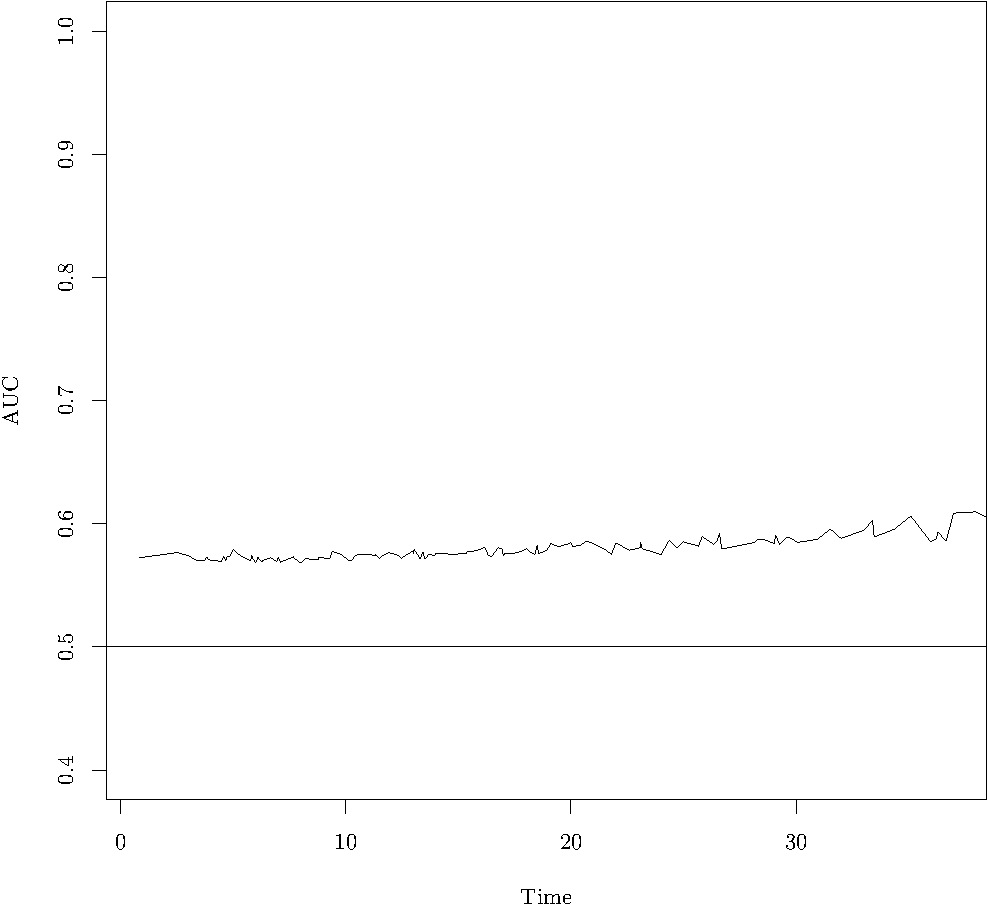
\includegraphics[width=\maxwidth]{figure/05-risksetROC-8} 

}


\begin{kframe}\begin{verbatim}
## $utimes
##   [1]   0.80   1.63   2.50   3.00   3.40   3.73   3.83   3.90   4.47   4.57
##  [11]   4.67   4.73   4.83   4.87   5.00   5.30   5.77   5.83   5.87   6.00
##  [21]   6.10   6.27   6.30   6.67   6.93   7.00   7.10   7.66   7.67   7.73
##  [31]   8.00   8.17   8.33   8.43   8.47   8.77   8.80   9.00   9.03   9.30
##  [41]   9.40   9.83  10.13  10.27  10.40  10.50  11.07  11.30  11.33  11.50
##  [51]  11.60  11.90  12.33  12.47  12.97  13.00  13.03  13.10  13.30  13.43
##  [61]  13.50  13.57  13.70  13.93  14.00  14.80  15.37  15.40  15.57  16.00
##  [71]  16.17  16.33  16.47  16.77  16.95  17.00  17.07  17.57  17.83  18.03
##  [81]  18.17  18.40  18.50  18.57  18.93  19.10  19.50  19.63  19.80  20.00
##  [91]  20.07  20.43  20.67  20.90  21.53  21.80  22.00  22.60  23.07  23.10
## [101]  23.17  24.00  24.37  24.70  25.00  25.67  25.83  26.33  26.40  26.50
## [111]  26.60  26.70  27.53  28.13  28.33  28.53  29.03  29.10  29.27  29.60
## [121]  29.67  30.07  30.97  31.00  31.53  32.00  33.00  33.10  33.40  33.47
## [131]  34.37  35.10  35.97  36.23  36.30  36.67  37.00  38.00  39.60  41.23
## [141]  43.07  45.37  46.67  47.43  47.73  48.00  49.00  51.00  54.90  59.00
## [151]  63.13  65.00  67.00  70.00  77.00  85.00  85.80  90.33  93.00  94.77
## [161] 116.00
## 
## $St
##   [1] 0.99476 0.98930 0.98383 0.97834 0.97284 0.96734 0.96185 0.95086
##   [9] 0.93986 0.93437 0.92887 0.92337 0.91788 0.90689 0.89589 0.89040
##  [17] 0.88490 0.87940 0.87391 0.86841 0.86291 0.85742 0.85192 0.84643
##  [25] 0.84093 0.83543 0.82994 0.82444 0.81894 0.81345 0.80246 0.79696
##  [33] 0.79146 0.78597 0.78047 0.77497 0.76948 0.76398 0.75845 0.75291
##  [41] 0.74737 0.74184 0.73630 0.73077 0.72523 0.71969 0.71416 0.70862
##  [49] 0.70308 0.69755 0.69201 0.68648 0.68094 0.67540 0.66987 0.66433
##  [57] 0.65880 0.65326 0.64772 0.64219 0.63665 0.63112 0.62558 0.62004
##  [65] 0.61451 0.60892 0.60333 0.59775 0.59216 0.58658 0.58099 0.57540
##  [73] 0.56982 0.56423 0.55864 0.55306 0.54747 0.54188 0.53630 0.53071
##  [81] 0.52512 0.51954 0.51395 0.50837 0.50278 0.49719 0.49161 0.48602
##  [89] 0.48043 0.46926 0.46367 0.45809 0.45250 0.44691 0.44133 0.43574
##  [97] 0.43016 0.42457 0.41898 0.41340 0.40781 0.39664 0.39105 0.38546
## [105] 0.37429 0.36870 0.36312 0.35753 0.35195 0.34636 0.34077 0.33519
## [113] 0.32960 0.32401 0.31843 0.31284 0.30725 0.30167 0.29608 0.29049
## [121] 0.28491 0.27932 0.27374 0.26815 0.26256 0.25698 0.25139 0.24580
## [129] 0.24022 0.23463 0.22904 0.22332 0.21759 0.21187 0.20614 0.20041
## [137] 0.19469 0.18289 0.17679 0.17048 0.16416 0.15760 0.15103 0.14446
## [145] 0.13790 0.13133 0.12442 0.11751 0.10967 0.10184 0.09401 0.08617
## [153] 0.07834 0.07050 0.06169 0.05141 0.04113 0.03085 0.02056 0.01028
## [161] 0.00000
## 
## $AUC
##   [1] 0.5723 0.5744 0.5766 0.5742 0.5699 0.5704 0.5729 0.5707 0.5694 0.5733
##  [11] 0.5701 0.5733 0.5732 0.5744 0.5792 0.5744 0.5699 0.5743 0.5718 0.5682
##  [21] 0.5726 0.5689 0.5701 0.5723 0.5692 0.5729 0.5689 0.5730 0.5732 0.5717
##  [31] 0.5680 0.5713 0.5724 0.5706 0.5709 0.5707 0.5726 0.5726 0.5719 0.5719
##  [41] 0.5776 0.5747 0.5700 0.5706 0.5736 0.5747 0.5754 0.5739 0.5752 0.5716
##  [51] 0.5735 0.5767 0.5744 0.5721 0.5778 0.5758 0.5791 0.5773 0.5717 0.5771
##  [61] 0.5716 0.5725 0.5753 0.5743 0.5760 0.5752 0.5759 0.5777 0.5774 0.5792
##  [71] 0.5811 0.5742 0.5734 0.5804 0.5796 0.5738 0.5759 0.5763 0.5778 0.5798
##  [81] 0.5771 0.5750 0.5825 0.5758 0.5784 0.5838 0.5812 0.5826 0.5830 0.5847
##  [91] 0.5817 0.5823 0.5862 0.5847 0.5791 0.5751 0.5844 0.5786 0.5805 0.5848
## [101] 0.5798 0.5749 0.5867 0.5802 0.5853 0.5819 0.5897 0.5834 0.5842 0.5865
## [111] 0.5923 0.5794 0.5826 0.5847 0.5876 0.5876 0.5839 0.5905 0.5831 0.5889
## [121] 0.5892 0.5848 0.5874 0.5882 0.5957 0.5881 0.5946 0.5966 0.6026 0.5892
## [131] 0.5956 0.6062 0.5856 0.5876 0.5931 0.5861 0.6086 0.6097 0.5945 0.5881
## [141] 0.6132 0.5807 0.5967 0.5913 0.5844 0.6111 0.5856 0.6234 0.6160 0.6236
## [151] 0.6229 0.5656 0.6111 0.6573 0.5917 0.5836 0.5309 0.4725 0.7439 0.2936
## [161] 0.0000
## 
## $Cindex
## [1] 0.576
\end{verbatim}
\begin{alltt}
\hlkwd{risksetAUC}\hlstd{(data.glasgow}\hlopt{$}\hlstd{Time}\hlopt{/}\hlnum{365.25}\hlopt{*}\hlnum{12}\hlstd{,} \hlkwc{status} \hlstd{= data.glasgow}\hlopt{$}\hlstd{DSD,} \hlkwc{marker} \hlstd{= gg.linpred.glasgow,} \hlkwc{tmax} \hlstd{=} \hlnum{36}\hlstd{)}
\end{alltt}
\end{kframe}

{\centering 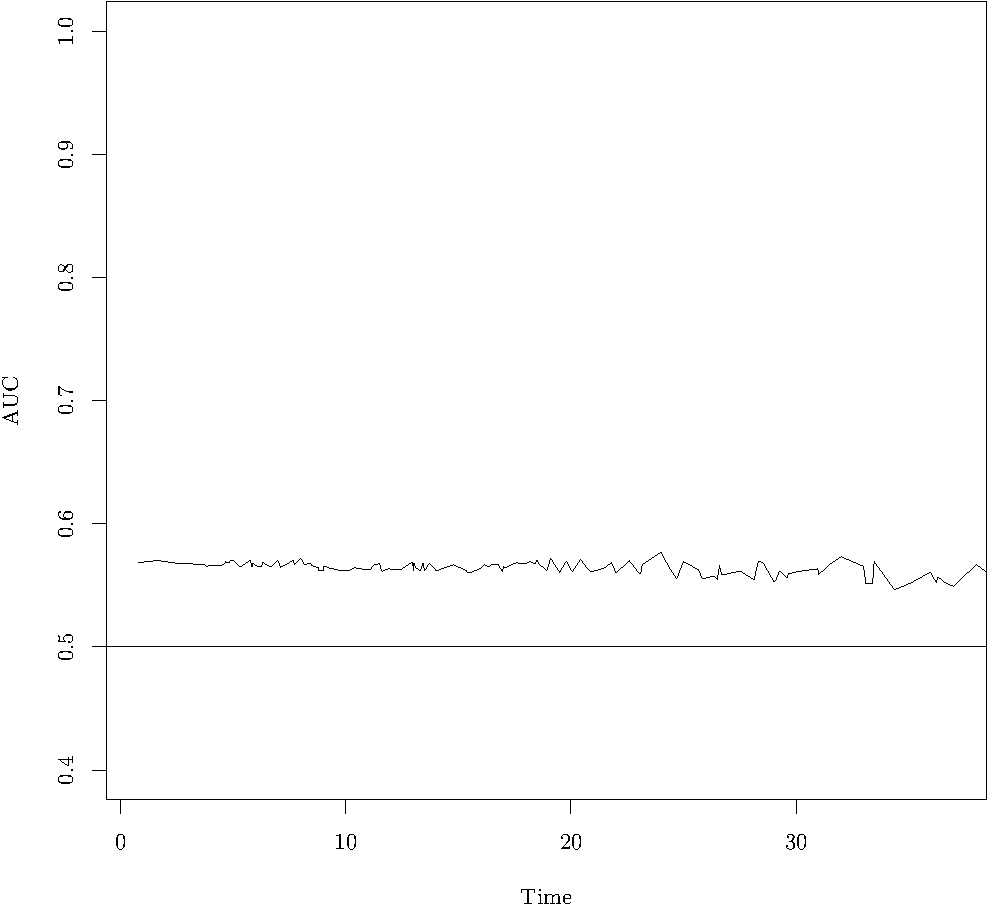
\includegraphics[width=\maxwidth]{figure/05-risksetROC-9} 

}


\begin{kframe}\begin{verbatim}
## $utimes
##   [1]   0.80   1.63   2.50   3.00   3.40   3.73   3.83   3.90   4.47   4.57
##  [11]   4.67   4.73   4.83   4.87   5.00   5.30   5.77   5.83   5.87   6.00
##  [21]   6.10   6.27   6.30   6.67   6.93   7.00   7.10   7.66   7.67   7.73
##  [31]   8.00   8.17   8.33   8.43   8.47   8.77   8.80   9.00   9.03   9.30
##  [41]   9.40   9.83  10.13  10.27  10.40  10.50  11.07  11.30  11.33  11.50
##  [51]  11.60  11.90  12.33  12.47  12.97  13.00  13.03  13.10  13.30  13.43
##  [61]  13.50  13.57  13.70  13.93  14.00  14.80  15.37  15.40  15.57  16.00
##  [71]  16.17  16.33  16.47  16.77  16.95  17.00  17.07  17.57  17.83  18.03
##  [81]  18.17  18.40  18.50  18.57  18.93  19.10  19.50  19.63  19.80  20.00
##  [91]  20.07  20.43  20.67  20.90  21.53  21.80  22.00  22.60  23.07  23.10
## [101]  23.17  24.00  24.37  24.70  25.00  25.67  25.83  26.33  26.40  26.50
## [111]  26.60  26.70  27.53  28.13  28.33  28.53  29.03  29.10  29.27  29.60
## [121]  29.67  30.07  30.97  31.00  31.53  32.00  33.00  33.10  33.40  33.47
## [131]  34.37  35.10  35.97  36.23  36.30  36.67  37.00  38.00  39.60  41.23
## [141]  43.07  45.37  46.67  47.43  47.73  48.00  49.00  51.00  54.90  59.00
## [151]  63.13  65.00  67.00  70.00  77.00  85.00  85.80  90.33  93.00  94.77
## [161] 116.00
## 
## $St
##   [1] 0.99476 0.98930 0.98383 0.97834 0.97284 0.96734 0.96185 0.95086
##   [9] 0.93986 0.93437 0.92887 0.92337 0.91788 0.90689 0.89589 0.89040
##  [17] 0.88490 0.87940 0.87391 0.86841 0.86291 0.85742 0.85192 0.84643
##  [25] 0.84093 0.83543 0.82994 0.82444 0.81894 0.81345 0.80246 0.79696
##  [33] 0.79146 0.78597 0.78047 0.77497 0.76948 0.76398 0.75845 0.75291
##  [41] 0.74737 0.74184 0.73630 0.73077 0.72523 0.71969 0.71416 0.70862
##  [49] 0.70308 0.69755 0.69201 0.68648 0.68094 0.67540 0.66987 0.66433
##  [57] 0.65880 0.65326 0.64772 0.64219 0.63665 0.63112 0.62558 0.62004
##  [65] 0.61451 0.60892 0.60333 0.59775 0.59216 0.58658 0.58099 0.57540
##  [73] 0.56982 0.56423 0.55864 0.55306 0.54747 0.54188 0.53630 0.53071
##  [81] 0.52512 0.51954 0.51395 0.50837 0.50278 0.49719 0.49161 0.48602
##  [89] 0.48043 0.46926 0.46367 0.45809 0.45250 0.44691 0.44133 0.43574
##  [97] 0.43016 0.42457 0.41898 0.41340 0.40781 0.39664 0.39105 0.38546
## [105] 0.37429 0.36870 0.36312 0.35753 0.35195 0.34636 0.34077 0.33519
## [113] 0.32960 0.32401 0.31843 0.31284 0.30725 0.30167 0.29608 0.29049
## [121] 0.28491 0.27932 0.27374 0.26815 0.26256 0.25698 0.25139 0.24580
## [129] 0.24022 0.23463 0.22904 0.22332 0.21759 0.21187 0.20614 0.20041
## [137] 0.19469 0.18289 0.17679 0.17048 0.16416 0.15760 0.15103 0.14446
## [145] 0.13790 0.13133 0.12442 0.11751 0.10967 0.10184 0.09401 0.08617
## [153] 0.07834 0.07050 0.06169 0.05141 0.04113 0.03085 0.02056 0.01028
## [161] 0.00000
## 
## $AUC
##   [1] 0.5917 0.5936 0.5912 0.5911 0.5899 0.5904 0.5879 0.5891 0.5894 0.5896
##  [11] 0.5920 0.5913 0.5911 0.5923 0.5924 0.5873 0.5928 0.5866 0.5902 0.5888
##  [21] 0.5880 0.5872 0.5910 0.5871 0.5918 0.5920 0.5869 0.5922 0.5907 0.5887
##  [31] 0.5935 0.5875 0.5887 0.5891 0.5871 0.5844 0.5836 0.5836 0.5850 0.5854
##  [41] 0.5838 0.5828 0.5833 0.5851 0.5851 0.5857 0.5839 0.5890 0.5890 0.5887
##  [51] 0.5829 0.5855 0.5841 0.5837 0.5905 0.5837 0.5893 0.5868 0.5830 0.5893
##  [61] 0.5840 0.5863 0.5889 0.5845 0.5833 0.5870 0.5832 0.5820 0.5819 0.5859
##  [71] 0.5876 0.5859 0.5875 0.5879 0.5829 0.5883 0.5853 0.5893 0.5902 0.5903
##  [81] 0.5902 0.5879 0.5926 0.5886 0.5837 0.5937 0.5816 0.5866 0.5907 0.5829
##  [91] 0.5826 0.5921 0.5872 0.5821 0.5843 0.5883 0.5810 0.5907 0.5792 0.5804
## [101] 0.5867 0.5976 0.5858 0.5752 0.5896 0.5809 0.5747 0.5782 0.5758 0.5744
## [111] 0.5857 0.5805 0.5790 0.5737 0.5884 0.5866 0.5699 0.5749 0.5788 0.5717
## [121] 0.5756 0.5780 0.5808 0.5747 0.5849 0.5919 0.5814 0.5680 0.5677 0.5861
## [131] 0.5629 0.5733 0.5817 0.5723 0.5696 0.5681 0.5654 0.5785 0.5647 0.5790
## [141] 0.5606 0.5945 0.5721 0.5641 0.5621 0.5586 0.5937 0.5741 0.5670 0.5571
## [151] 0.6063 0.5946 0.5687 0.5307 0.5078 0.5116 0.4663 0.5029 0.7187 0.7616
## [161] 0.0000
## 
## $Cindex
## [1] 0.587
\end{verbatim}
\begin{alltt}
\hlkwd{risksetAUC}\hlstd{(data.glasgow}\hlopt{$}\hlstd{Time}\hlopt{/}\hlnum{365.25}\hlopt{*}\hlnum{12}\hlstd{,} \hlkwc{status} \hlstd{= data.glasgow}\hlopt{$}\hlstd{DSD,} \hlkwc{marker} \hlstd{= gg2.linpred.glasgow,} \hlkwc{tmax} \hlstd{=} \hlnum{36}\hlstd{)}
\end{alltt}
\end{kframe}

{\centering 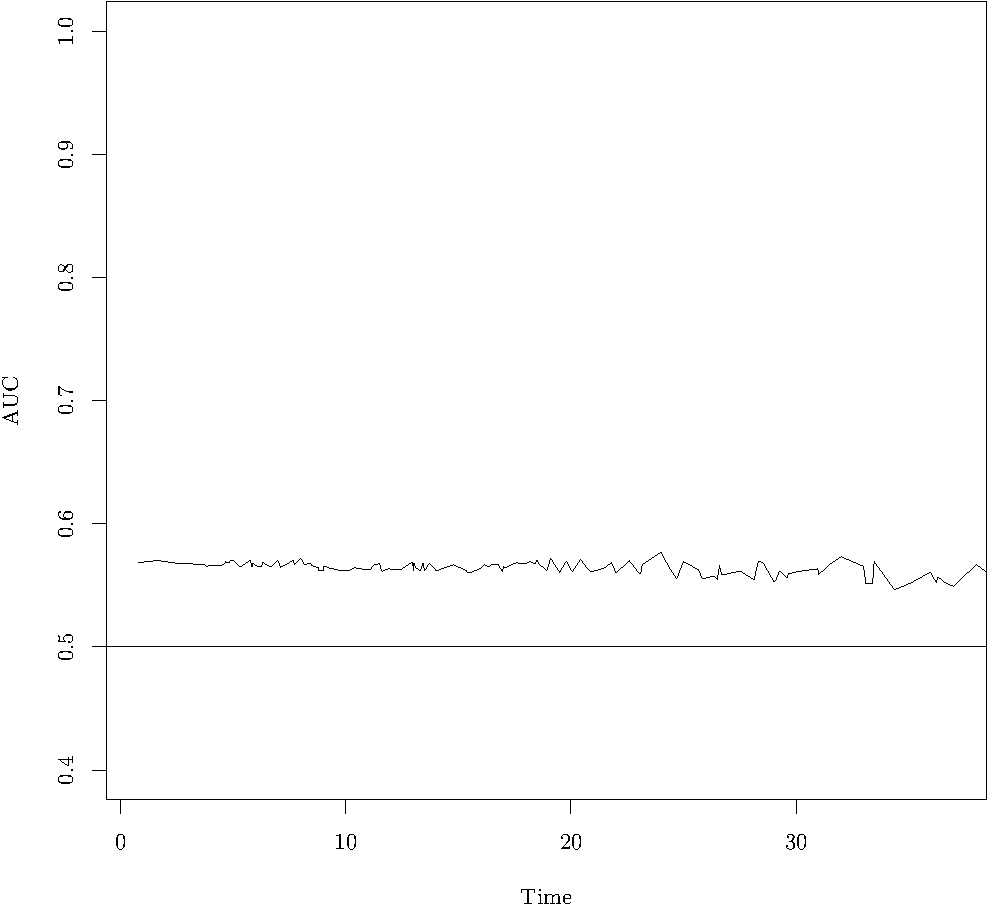
\includegraphics[width=\maxwidth]{figure/05-risksetROC-10} 

}


\begin{kframe}\begin{verbatim}
## $utimes
##   [1]   0.80   1.63   2.50   3.00   3.40   3.73   3.83   3.90   4.47   4.57
##  [11]   4.67   4.73   4.83   4.87   5.00   5.30   5.77   5.83   5.87   6.00
##  [21]   6.10   6.27   6.30   6.67   6.93   7.00   7.10   7.66   7.67   7.73
##  [31]   8.00   8.17   8.33   8.43   8.47   8.77   8.80   9.00   9.03   9.30
##  [41]   9.40   9.83  10.13  10.27  10.40  10.50  11.07  11.30  11.33  11.50
##  [51]  11.60  11.90  12.33  12.47  12.97  13.00  13.03  13.10  13.30  13.43
##  [61]  13.50  13.57  13.70  13.93  14.00  14.80  15.37  15.40  15.57  16.00
##  [71]  16.17  16.33  16.47  16.77  16.95  17.00  17.07  17.57  17.83  18.03
##  [81]  18.17  18.40  18.50  18.57  18.93  19.10  19.50  19.63  19.80  20.00
##  [91]  20.07  20.43  20.67  20.90  21.53  21.80  22.00  22.60  23.07  23.10
## [101]  23.17  24.00  24.37  24.70  25.00  25.67  25.83  26.33  26.40  26.50
## [111]  26.60  26.70  27.53  28.13  28.33  28.53  29.03  29.10  29.27  29.60
## [121]  29.67  30.07  30.97  31.00  31.53  32.00  33.00  33.10  33.40  33.47
## [131]  34.37  35.10  35.97  36.23  36.30  36.67  37.00  38.00  39.60  41.23
## [141]  43.07  45.37  46.67  47.43  47.73  48.00  49.00  51.00  54.90  59.00
## [151]  63.13  65.00  67.00  70.00  77.00  85.00  85.80  90.33  93.00  94.77
## [161] 116.00
## 
## $St
##   [1] 0.99476 0.98930 0.98383 0.97834 0.97284 0.96734 0.96185 0.95086
##   [9] 0.93986 0.93437 0.92887 0.92337 0.91788 0.90689 0.89589 0.89040
##  [17] 0.88490 0.87940 0.87391 0.86841 0.86291 0.85742 0.85192 0.84643
##  [25] 0.84093 0.83543 0.82994 0.82444 0.81894 0.81345 0.80246 0.79696
##  [33] 0.79146 0.78597 0.78047 0.77497 0.76948 0.76398 0.75845 0.75291
##  [41] 0.74737 0.74184 0.73630 0.73077 0.72523 0.71969 0.71416 0.70862
##  [49] 0.70308 0.69755 0.69201 0.68648 0.68094 0.67540 0.66987 0.66433
##  [57] 0.65880 0.65326 0.64772 0.64219 0.63665 0.63112 0.62558 0.62004
##  [65] 0.61451 0.60892 0.60333 0.59775 0.59216 0.58658 0.58099 0.57540
##  [73] 0.56982 0.56423 0.55864 0.55306 0.54747 0.54188 0.53630 0.53071
##  [81] 0.52512 0.51954 0.51395 0.50837 0.50278 0.49719 0.49161 0.48602
##  [89] 0.48043 0.46926 0.46367 0.45809 0.45250 0.44691 0.44133 0.43574
##  [97] 0.43016 0.42457 0.41898 0.41340 0.40781 0.39664 0.39105 0.38546
## [105] 0.37429 0.36870 0.36312 0.35753 0.35195 0.34636 0.34077 0.33519
## [113] 0.32960 0.32401 0.31843 0.31284 0.30725 0.30167 0.29608 0.29049
## [121] 0.28491 0.27932 0.27374 0.26815 0.26256 0.25698 0.25139 0.24580
## [129] 0.24022 0.23463 0.22904 0.22332 0.21759 0.21187 0.20614 0.20041
## [137] 0.19469 0.18289 0.17679 0.17048 0.16416 0.15760 0.15103 0.14446
## [145] 0.13790 0.13133 0.12442 0.11751 0.10967 0.10184 0.09401 0.08617
## [153] 0.07834 0.07050 0.06169 0.05141 0.04113 0.03085 0.02056 0.01028
## [161] 0.00000
## 
## $AUC
##   [1] 0.5872 0.5891 0.5865 0.5865 0.5855 0.5859 0.5834 0.5848 0.5850 0.5851
##  [11] 0.5877 0.5869 0.5867 0.5880 0.5880 0.5830 0.5885 0.5824 0.5860 0.5843
##  [21] 0.5835 0.5832 0.5868 0.5829 0.5875 0.5877 0.5824 0.5879 0.5865 0.5844
##  [31] 0.5893 0.5834 0.5845 0.5849 0.5829 0.5803 0.5792 0.5789 0.5814 0.5811
##  [41] 0.5800 0.5786 0.5789 0.5809 0.5810 0.5815 0.5797 0.5847 0.5847 0.5844
##  [51] 0.5786 0.5812 0.5796 0.5798 0.5862 0.5791 0.5850 0.5824 0.5785 0.5850
##  [61] 0.5798 0.5813 0.5846 0.5802 0.5785 0.5828 0.5786 0.5776 0.5776 0.5816
##  [71] 0.5831 0.5814 0.5832 0.5835 0.5785 0.5839 0.5812 0.5848 0.5856 0.5858
##  [81] 0.5858 0.5843 0.5883 0.5844 0.5794 0.5894 0.5774 0.5824 0.5864 0.5788
##  [91] 0.5781 0.5879 0.5829 0.5772 0.5805 0.5846 0.5768 0.5865 0.5751 0.5758
## [101] 0.5825 0.5936 0.5811 0.5708 0.5851 0.5772 0.5705 0.5726 0.5715 0.5702
## [111] 0.5815 0.5760 0.5759 0.5696 0.5844 0.5828 0.5657 0.5683 0.5749 0.5684
## [121] 0.5725 0.5746 0.5770 0.5715 0.5812 0.5880 0.5778 0.5643 0.5646 0.5826
## [131] 0.5594 0.5651 0.5783 0.5652 0.5684 0.5647 0.5626 0.5780 0.5611 0.5759
## [141] 0.5573 0.5910 0.5591 0.5624 0.5586 0.5554 0.5895 0.5671 0.5626 0.5428
## [151] 0.6005 0.5901 0.5644 0.5257 0.5028 0.5057 0.4610 0.5008 0.7164 0.7613
## [161] 0.0000
## 
## $Cindex
## [1] 0.5827
\end{verbatim}
\begin{alltt}
\hlkwd{risksetAUC}\hlstd{(data.glasgow}\hlopt{$}\hlstd{Time}\hlopt{/}\hlnum{365.25}\hlopt{*}\hlnum{12}\hlstd{,} \hlkwc{status} \hlstd{= data.glasgow}\hlopt{$}\hlstd{DSD,} \hlkwc{marker} \hlstd{= cph.linpred.glasgow,} \hlkwc{tmax} \hlstd{=} \hlnum{36}\hlstd{)}
\end{alltt}
\end{kframe}

{\centering 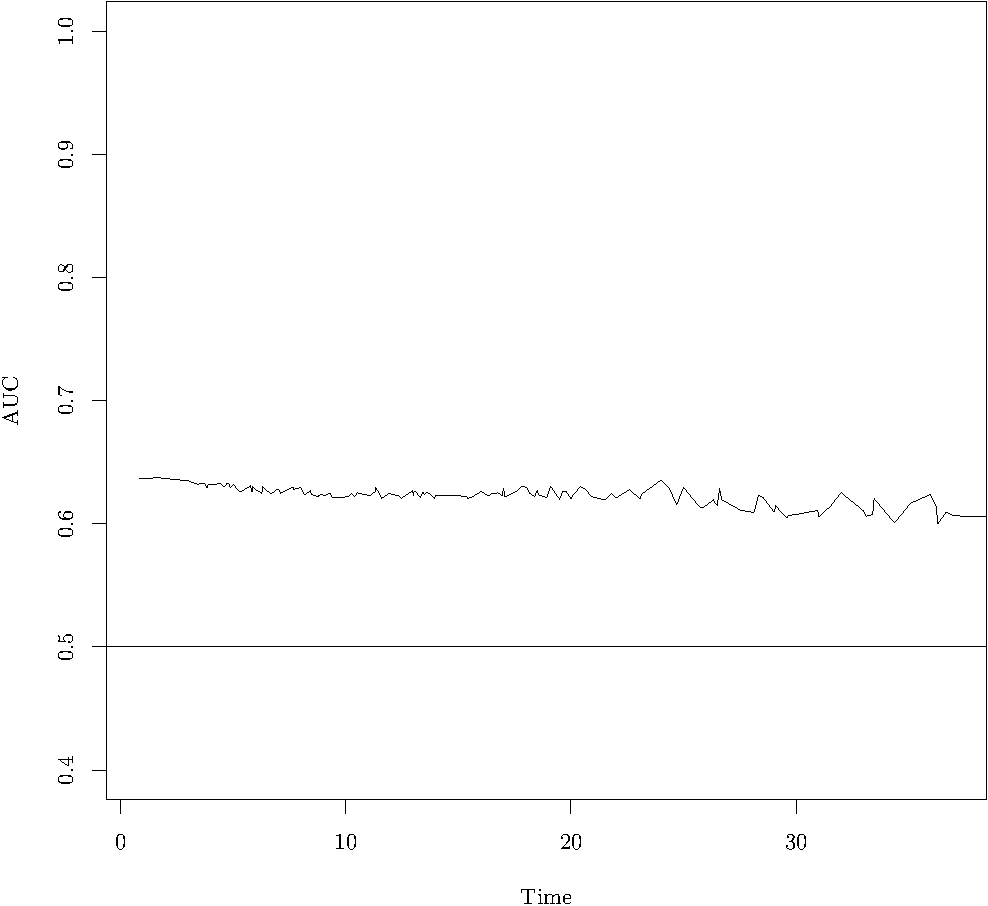
\includegraphics[width=\maxwidth]{figure/05-risksetROC-11} 

}


\begin{kframe}\begin{verbatim}
## $utimes
##   [1]   0.80   1.63   2.50   3.00   3.40   3.73   3.83   3.90   4.47   4.57
##  [11]   4.67   4.73   4.83   4.87   5.00   5.30   5.77   5.83   5.87   6.00
##  [21]   6.10   6.27   6.30   6.67   6.93   7.00   7.10   7.66   7.67   7.73
##  [31]   8.00   8.17   8.33   8.43   8.47   8.77   8.80   9.00   9.03   9.30
##  [41]   9.40   9.83  10.13  10.27  10.40  10.50  11.07  11.30  11.33  11.50
##  [51]  11.60  11.90  12.33  12.47  12.97  13.00  13.03  13.10  13.30  13.43
##  [61]  13.50  13.57  13.70  13.93  14.00  14.80  15.37  15.40  15.57  16.00
##  [71]  16.17  16.33  16.47  16.77  16.95  17.00  17.07  17.57  17.83  18.03
##  [81]  18.17  18.40  18.50  18.57  18.93  19.10  19.50  19.63  19.80  20.00
##  [91]  20.07  20.43  20.67  20.90  21.53  21.80  22.00  22.60  23.07  23.10
## [101]  23.17  24.00  24.37  24.70  25.00  25.67  25.83  26.33  26.40  26.50
## [111]  26.60  26.70  27.53  28.13  28.33  28.53  29.03  29.10  29.27  29.60
## [121]  29.67  30.07  30.97  31.00  31.53  32.00  33.00  33.10  33.40  33.47
## [131]  34.37  35.10  35.97  36.23  36.30  36.67  37.00  38.00  39.60  41.23
## [141]  43.07  45.37  46.67  47.43  47.73  48.00  49.00  51.00  54.90  59.00
## [151]  63.13  65.00  67.00  70.00  77.00  85.00  85.80  90.33  93.00  94.77
## [161] 116.00
## 
## $St
##   [1] 0.99476 0.98930 0.98383 0.97834 0.97284 0.96734 0.96185 0.95086
##   [9] 0.93986 0.93437 0.92887 0.92337 0.91788 0.90689 0.89589 0.89040
##  [17] 0.88490 0.87940 0.87391 0.86841 0.86291 0.85742 0.85192 0.84643
##  [25] 0.84093 0.83543 0.82994 0.82444 0.81894 0.81345 0.80246 0.79696
##  [33] 0.79146 0.78597 0.78047 0.77497 0.76948 0.76398 0.75845 0.75291
##  [41] 0.74737 0.74184 0.73630 0.73077 0.72523 0.71969 0.71416 0.70862
##  [49] 0.70308 0.69755 0.69201 0.68648 0.68094 0.67540 0.66987 0.66433
##  [57] 0.65880 0.65326 0.64772 0.64219 0.63665 0.63112 0.62558 0.62004
##  [65] 0.61451 0.60892 0.60333 0.59775 0.59216 0.58658 0.58099 0.57540
##  [73] 0.56982 0.56423 0.55864 0.55306 0.54747 0.54188 0.53630 0.53071
##  [81] 0.52512 0.51954 0.51395 0.50837 0.50278 0.49719 0.49161 0.48602
##  [89] 0.48043 0.46926 0.46367 0.45809 0.45250 0.44691 0.44133 0.43574
##  [97] 0.43016 0.42457 0.41898 0.41340 0.40781 0.39664 0.39105 0.38546
## [105] 0.37429 0.36870 0.36312 0.35753 0.35195 0.34636 0.34077 0.33519
## [113] 0.32960 0.32401 0.31843 0.31284 0.30725 0.30167 0.29608 0.29049
## [121] 0.28491 0.27932 0.27374 0.26815 0.26256 0.25698 0.25139 0.24580
## [129] 0.24022 0.23463 0.22904 0.22332 0.21759 0.21187 0.20614 0.20041
## [137] 0.19469 0.18289 0.17679 0.17048 0.16416 0.15760 0.15103 0.14446
## [145] 0.13790 0.13133 0.12442 0.11751 0.10967 0.10184 0.09401 0.08617
## [153] 0.07834 0.07050 0.06169 0.05141 0.04113 0.03085 0.02056 0.01028
## [161] 0.00000
## 
## $AUC
##   [1] 0.6348 0.6358 0.6345 0.6336 0.6311 0.6314 0.6280 0.6309 0.6312 0.6290
##  [11] 0.6297 0.6319 0.6306 0.6277 0.6307 0.6243 0.6295 0.6243 0.6291 0.6262
##  [21] 0.6255 0.6234 0.6290 0.6231 0.6265 0.6271 0.6236 0.6284 0.6263 0.6267
##  [31] 0.6279 0.6218 0.6237 0.6251 0.6221 0.6195 0.6211 0.6213 0.6206 0.6230
##  [41] 0.6188 0.6193 0.6203 0.6225 0.6199 0.6230 0.6209 0.6239 0.6276 0.6223
##  [51] 0.6189 0.6226 0.6213 0.6190 0.6255 0.6209 0.6242 0.6245 0.6195 0.6240
##  [61] 0.6213 0.6228 0.6226 0.6182 0.6204 0.6206 0.6198 0.6182 0.6190 0.6239
##  [71] 0.6217 0.6201 0.6220 0.6225 0.6200 0.6265 0.6192 0.6234 0.6278 0.6266
##  [81] 0.6215 0.6195 0.6244 0.6201 0.6181 0.6272 0.6166 0.6228 0.6225 0.6166
##  [91] 0.6192 0.6263 0.6235 0.6177 0.6149 0.6209 0.6163 0.6229 0.6152 0.6174
## [101] 0.6194 0.6301 0.6226 0.6085 0.6229 0.6077 0.6057 0.6127 0.6099 0.6084
## [111] 0.6217 0.6121 0.6043 0.6025 0.6167 0.6142 0.6013 0.6067 0.6029 0.5968
## [121] 0.5989 0.6003 0.6036 0.5980 0.6071 0.6180 0.6025 0.5982 0.5997 0.6124
## [131] 0.5937 0.6099 0.6169 0.6055 0.5918 0.6020 0.5988 0.5986 0.5994 0.6199
## [141] 0.5977 0.6297 0.6181 0.5967 0.5940 0.6054 0.6296 0.6304 0.6070 0.6401
## [151] 0.6681 0.6143 0.5833 0.5562 0.5800 0.5561 0.5162 0.5436 0.7619 0.7673
## [161] 0.0000
## 
## $Cindex
## [1] 0.6229
\end{verbatim}
\begin{alltt}
\hlkwd{risksetAUC}\hlstd{(data.glasgow}\hlopt{$}\hlstd{Time}\hlopt{/}\hlnum{365.25}\hlopt{*}\hlnum{12}\hlstd{,} \hlkwc{status} \hlstd{= data.glasgow}\hlopt{$}\hlstd{DSD,} \hlkwc{marker} \hlstd{= rsf.linpred.glasgow,} \hlkwc{tmax} \hlstd{=} \hlnum{36}\hlstd{)}
\end{alltt}
\end{kframe}

{\centering 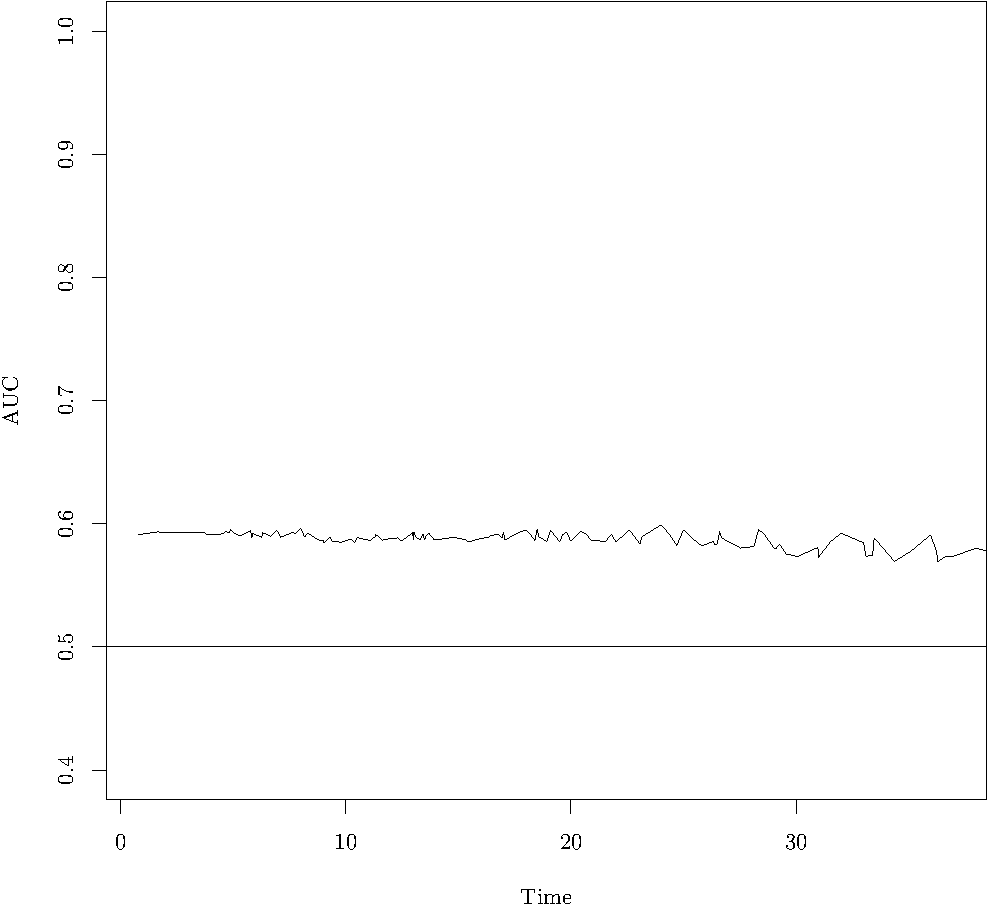
\includegraphics[width=\maxwidth]{figure/05-risksetROC-12} 

}


\begin{kframe}\begin{verbatim}
## $utimes
##   [1]   0.80   1.63   2.50   3.00   3.40   3.73   3.83   3.90   4.47   4.57
##  [11]   4.67   4.73   4.83   4.87   5.00   5.30   5.77   5.83   5.87   6.00
##  [21]   6.10   6.27   6.30   6.67   6.93   7.00   7.10   7.66   7.67   7.73
##  [31]   8.00   8.17   8.33   8.43   8.47   8.77   8.80   9.00   9.03   9.30
##  [41]   9.40   9.83  10.13  10.27  10.40  10.50  11.07  11.30  11.33  11.50
##  [51]  11.60  11.90  12.33  12.47  12.97  13.00  13.03  13.10  13.30  13.43
##  [61]  13.50  13.57  13.70  13.93  14.00  14.80  15.37  15.40  15.57  16.00
##  [71]  16.17  16.33  16.47  16.77  16.95  17.00  17.07  17.57  17.83  18.03
##  [81]  18.17  18.40  18.50  18.57  18.93  19.10  19.50  19.63  19.80  20.00
##  [91]  20.07  20.43  20.67  20.90  21.53  21.80  22.00  22.60  23.07  23.10
## [101]  23.17  24.00  24.37  24.70  25.00  25.67  25.83  26.33  26.40  26.50
## [111]  26.60  26.70  27.53  28.13  28.33  28.53  29.03  29.10  29.27  29.60
## [121]  29.67  30.07  30.97  31.00  31.53  32.00  33.00  33.10  33.40  33.47
## [131]  34.37  35.10  35.97  36.23  36.30  36.67  37.00  38.00  39.60  41.23
## [141]  43.07  45.37  46.67  47.43  47.73  48.00  49.00  51.00  54.90  59.00
## [151]  63.13  65.00  67.00  70.00  77.00  85.00  85.80  90.33  93.00  94.77
## [161] 116.00
## 
## $St
##   [1] 0.99476 0.98930 0.98383 0.97834 0.97284 0.96734 0.96185 0.95086
##   [9] 0.93986 0.93437 0.92887 0.92337 0.91788 0.90689 0.89589 0.89040
##  [17] 0.88490 0.87940 0.87391 0.86841 0.86291 0.85742 0.85192 0.84643
##  [25] 0.84093 0.83543 0.82994 0.82444 0.81894 0.81345 0.80246 0.79696
##  [33] 0.79146 0.78597 0.78047 0.77497 0.76948 0.76398 0.75845 0.75291
##  [41] 0.74737 0.74184 0.73630 0.73077 0.72523 0.71969 0.71416 0.70862
##  [49] 0.70308 0.69755 0.69201 0.68648 0.68094 0.67540 0.66987 0.66433
##  [57] 0.65880 0.65326 0.64772 0.64219 0.63665 0.63112 0.62558 0.62004
##  [65] 0.61451 0.60892 0.60333 0.59775 0.59216 0.58658 0.58099 0.57540
##  [73] 0.56982 0.56423 0.55864 0.55306 0.54747 0.54188 0.53630 0.53071
##  [81] 0.52512 0.51954 0.51395 0.50837 0.50278 0.49719 0.49161 0.48602
##  [89] 0.48043 0.46926 0.46367 0.45809 0.45250 0.44691 0.44133 0.43574
##  [97] 0.43016 0.42457 0.41898 0.41340 0.40781 0.39664 0.39105 0.38546
## [105] 0.37429 0.36870 0.36312 0.35753 0.35195 0.34636 0.34077 0.33519
## [113] 0.32960 0.32401 0.31843 0.31284 0.30725 0.30167 0.29608 0.29049
## [121] 0.28491 0.27932 0.27374 0.26815 0.26256 0.25698 0.25139 0.24580
## [129] 0.24022 0.23463 0.22904 0.22332 0.21759 0.21187 0.20614 0.20041
## [137] 0.19469 0.18289 0.17679 0.17048 0.16416 0.15760 0.15103 0.14446
## [145] 0.13790 0.13133 0.12442 0.11751 0.10967 0.10184 0.09401 0.08617
## [153] 0.07834 0.07050 0.06169 0.05141 0.04113 0.03085 0.02056 0.01028
## [161] 0.00000
## 
## $AUC
##   [1] 0.5912 0.5934 0.5928 0.5928 0.5926 0.5929 0.5907 0.5914 0.5917 0.5924
##  [11] 0.5943 0.5931 0.5931 0.5953 0.5927 0.5901 0.5943 0.5889 0.5925 0.5908
##  [21] 0.5905 0.5889 0.5929 0.5896 0.5947 0.5935 0.5891 0.5931 0.5929 0.5919
##  [31] 0.5961 0.5893 0.5925 0.5910 0.5905 0.5871 0.5867 0.5866 0.5846 0.5888
##  [41] 0.5853 0.5851 0.5869 0.5872 0.5848 0.5888 0.5864 0.5893 0.5914 0.5886
##  [51] 0.5866 0.5878 0.5885 0.5860 0.5926 0.5868 0.5931 0.5893 0.5870 0.5919
##  [61] 0.5868 0.5901 0.5921 0.5868 0.5870 0.5890 0.5867 0.5857 0.5859 0.5882
##  [71] 0.5885 0.5891 0.5908 0.5911 0.5885 0.5932 0.5868 0.5920 0.5941 0.5942
##  [81] 0.5922 0.5864 0.5958 0.5896 0.5856 0.5946 0.5855 0.5910 0.5931 0.5857
##  [91] 0.5873 0.5939 0.5916 0.5867 0.5856 0.5915 0.5852 0.5949 0.5836 0.5863
## [101] 0.5897 0.5990 0.5917 0.5824 0.5949 0.5838 0.5822 0.5856 0.5829 0.5835
## [111] 0.5934 0.5884 0.5803 0.5815 0.5951 0.5929 0.5800 0.5796 0.5836 0.5745
## [121] 0.5751 0.5734 0.5808 0.5729 0.5853 0.5924 0.5845 0.5736 0.5742 0.5887
## [131] 0.5694 0.5777 0.5909 0.5783 0.5694 0.5736 0.5736 0.5803 0.5721 0.5825
## [141] 0.5727 0.6051 0.5843 0.5746 0.5651 0.5766 0.6048 0.6004 0.5725 0.5879
## [151] 0.6248 0.6103 0.5687 0.5463 0.5708 0.5377 0.4885 0.5096 0.7256 0.7552
## [161] 0.0000
## 
## $Cindex
## [1] 0.5897
\end{verbatim}
\end{kframe}
\end{knitrout}

\end{document}
